%%%%%%%%%%%%%%%%%%%%%%%%%%%%%%%%%%%%%%%%%%%%%%%%%%%%%%%%%%%%%%%%%%%%%%%%%%%%%
%$HeadURL: https://www.mech.kth.se/svn/simson/trunk/doc/simson-user-guide.tex $
%$LastChangedDate: 2008-09-16 22:40:07 +0200 (Tue, 16 Sep 2008) $
%$LastChangedBy: pschlatt@MECH.KTH.SE $
%$LastChangedRevision: 1291 $
%%%%%%%%%%%%%%%%%%%%%%%%%%%%%%%%%%%%%%%%%%%%%%%%%%%%%%%%%%%%%%%%%%%%%%%%%%%%%
%
% To compile this document do the following:
%
%   pdflatex simson-user-guide
%   bibtex simson-user-guide
%   pdflatex simson-user-guide
%   pdflatex simson-user-guide
%
%%%%%%%%%%%%%%%%%%%%%%%%%%%%%%%%%%%%%%%%%%%%%%%%%%%%%%%%%%%%%%%%%%%%%%%%%%%%%

\documentclass[10pt,a4paper]{simson}
\usepackage{natbib}
\usepackage{amsmath}
\usepackage{amsfonts}
\usepackage[colorlinks=true, pdfstartview=FitV, linkcolor=blue, citecolor=blue, urlcolor=blue, pdfauthor={Mattias Chevalier, Philipp Schlatter, Anders Lundbladh and Dan S. Henningson}, pdfkeywords={DNS, spectral, Fourier, Chebyshev, Simson}, pdftitle={Simson User Guide. Produced from $Rev: 1291 $}]{hyperref}

%%%%%%%%%%%%%%%%%%%%%%%%%%%%%%%%%%%%%%%%%%%%%%%%%%%%%%%%%%%%%%%%%%%%%%%%%%%%%%%
%
%   Symbols   Symbols   Symbols   Symbols   Symbols   Symbols   Symbols
%
%   (c) Copyright, 1985 by Moon J. Lee
%
%%%%%%%%%%%%%%%%%%%%%%%%%%%%%%%%%%%%%%%%%%%%%%%%%%%%%%%%%%%%%%%%%%%%%%%%%%%%%%%
%
\font\smallfont=cmsy10 at 10truept
\textfont8=\smallfont
\mathchardef\bigCircle="280D

\font\bigfont=cmsy10 at 14.4truept
\textfont9=\bigfont
\mathchardef\tiMes="2902        %

\font\Bigfont=cmsy10 at 17.28truept
\textfont10=\Bigfont
\mathchardef\DiaMond="2A05        %
%\mathchardef\buLlet="2A0F
\mathchardef\cirCle="2A0E
\mathchardef\BigCircle="2A0D

\font\Bbigfont=cmsy10 at 24.88truept
\textfont11=\Bbigfont
\mathchardef\buLLet="2B0F

%------------------------------------------------------------------------------%

\def\bigCirc{\raise 0.3ex\hbox{$\bigCircle$}\nobreak$\,$}
\def\Bigcirc{$\BigCircle$}                    %   very big circle (0.2" Diam.)
\def\Circ{\hbox{$\cirCle$}\nobreak$\,$}
\def\Bullet{\raise-0.35ex\hbox{$\buLLet$}\nobreak$\,$}
\def\triangleup{$\bigtriangleup$\nobreak$\,$}
\def\triangledown{\raise 0.2em\hbox{$\bigtriangledown$}\nobreak$\,$}
\def\uptriangle{\triangleup}       \def\downtriangle{\triangledown}
\def\Diamond{$\DiaMond$\nobreak$\,$}

\def\minisquare{\hbox{${\vcenter{
               \hrule height 0.3pt \kern-0.4pt
               \hbox{\vrule width  0.3pt height 3.0pt \kern 2.6pt
               \vrule width  0.3pt height 3.0pt} \kern-0.4pt
               \hrule height 0.3pt}}$}}
%\def\square{\raise 0.175ex\hbox{${\vcenter{
%               \hrule height 0.8truept       \kern-0.4truept
%               \hbox{\vrule width 0.8truept height 8.0truept \kern 7.6truept
%                     \vrule width 0.8truept height 8.0truept} \kern-0.4truept
%               \hrule height 0.8truept}}$}\nobreak$\,$}
\def\ssquare{\raise 0.175ex\hbox{${\vcenter{
               \hrule height 0.5truept       \kern-0.25truept
               \hbox{\vrule width 0.5truept height 3.0truept \kern 2.75truept
                     \vrule width 0.5truept height 3.0truept} \kern-0.25truept
               \hrule height 0.5truept}}$}\nobreak$\,$}
\def\squarex{\raise 0.175ex\hbox{${\vcenter{
               \hrule height 0.8truept       \kern-1.80truept
          \hbox{\vrule width 0.8truept height 8.0truept \kern-1.95truept
                \raise 0.8truept\hbox{$\tiMes$}     \kern-6.70truept
                \vrule width 0.8truept height 8.0truept} \kern-0.80truept
               \hrule height 0.8truept}}$}\nobreak$\,$}

\def\sqbull{\raise0.175ex\hbox{\vrule height 1.4ex width 1.6ex depth 0.2ex}\nobreak$\,$}
\def\smsqbull{\raise0.175ex\hbox{\vrule height 0.8ex width 0.9ex depth 0.2ex}\nobreak$\,$}

\def\Diamondplus{${\vcenter{\vcenter{\DiaMond} \kern-10truept
                            \hbox{\vrule width .4truept}\kern -3truept
                            \hrule height .4truept}}$\nobreak$\,$}
%
%%%%%%%%%%%%%%%%%%%%%%%%%%%%%%%%%%%%%%%%%%%%%%%%%%%%%%%%%%%%%%%%%%%%%%%%%%%%%%%
%
%         Lines   Lines   Lines   Lines   Lines   Lines   Lines
%
%%%%%%%%%%%%%%%%%%%%%%%%%%%%%%%%%%%%%%%%%%%%%%%%%%%%%%%%%%%%%%%%%%%%%%%%%%%%%%%
\newcount\ndots

\def\drawline#1#2{\raise 2.5truept\vbox{\hrule width #1truept height #2truept}}
\def\moonspace#1{\hskip #1truept}

\def\shortchain{\drawline{6.0}{0.75}}     
\def\chain{\drawline{12.0}{0.75}}     
\def\thinchain{\drawline{12.0}{0.25}}     
\def\chainspace{\chain\moonspace{2}}
\def\shortchainspace{\shortchain\moonspace{2}}
\def\thinchainspace{\thinchain\moonspace{2}}
\def\dashy{\drawline{4.00}{0.76}}     
\def\thindashy{\drawline{4.00}{0.25}}     
\def\dashyspace{\dashy\moonspace{2}}
\def\thindashyspace{\thindashy\moonspace{2}}
\def\longdashy{\drawline{8.00}{0.76}} 
\def\thinlongdashy{\drawline{8.00}{0.25}} 
\def\longdashyspace{\longdashy\moonspace{2}}
\def\thinlongdashyspace{\thinlongdashy\moonspace{2}}
\def\dotty{\drawline{1.00}{0.75}}     
\def\thindotty{\drawline{1.00}{0.25}}     
\def\dottyspace{\dotty\moonspace{2}}

\def\solid{\drawline{24}{0.75}\nobreak$\,$}  
\def\Solid{\drawline{24}{1.00}\nobreak$\,$}  
\def\thinsolid{\drawline{24}{0.25}\nobreak$\,$}  
\def\circthinsolid{$\circ$\drawline{6}{0.25}$\circ$\drawline{6}{0.25}$\circ$\nobreak$\,$}  

\def\circthinsolidpict{\begin{picture}(10,2)\linethickness{0.5pt}\put(0,1){\circle{3}}\put(0.5,1){\line(1,0){3}}\put(3.8,1){\circle{3}}\put(4.5,1){\line(1,0){3}}\put(7.8,1){\circle{3}}\end{picture}}  

\def\thinsolidpict{\begin{picture}(10,2)\linethickness{0.5pt}\put(0,1){\line(1,0){8}}\end{picture}}  

\def\thicksolidpict{\begin{picture}(10,2)\linethickness{1pt}\put(0,1){\line(1,0){8}}\end{picture}} 

\def\thindashedpict{\begin{picture}(11,2)\linethickness{0.5pt}\put(0,1){\line(1,0){2}}\put(2.5,1){\line(1,0){2}}\put(5,1){\line(1,0){2}}\put(7.5,1){\line(1,0){2}}\end{picture}}  

\def\dashedpict{\begin{picture}(11,2)\linethickness{0.75pt}\put(0,1){\line(1,0){2}}\put(2.5,1){\line(1,0){2}}\put(5,1){\line(1,0){2}}\put(7.5,1){\line(1,0){2}}\end{picture}}  

\def\squarethinsolidpict{\begin{picture}(10,2)\linethickness{0.5pt}\put(0,0.3){{\tiny $\square$}}\put(1.5,1){\line(1,0){2}}\put(3.3,0.3){{\tiny $\square$}}\put(4.7,1){\line(1,0){2}}\put(6.3,0.3){{\tiny $\square$}}\end{picture}}  

\def\diamondthinsolidpict{\begin{picture}(10,2)\linethickness{0.5pt}\put(0,0.3){{\small $\diamond$}}\put(1.5,1){\line(1,0){2}}\put(3.3,0.3){{\small $\diamond$}}\put(4.7,1){\line(1,0){2}}\put(6.3,0.3){{\small $\diamond$}}\end{picture}}  

%  ---------------------------

\def\dotbox{\hbox{\dottyspace}}
\def\dotted{\hbox{\leaders\dotbox\hskip 24truept}\nobreak$\,$}  
%  .  .  .  .  .  .  .  .  .  .

\def\dashbox{\hbox{\dashyspace}}  
\def\dashed{\hbox {\ndots=0 \loop\ifnum\ndots<3\advance\ndots by 1
        \dashbox\repeat\dashy}\nobreak$\,$}       
\def\thindashed{\hbox {\ndots=0 \loop\ifnum\ndots<3\advance\ndots by 1
        \dashbox\repeat\thindashy}\nobreak$\,$}       
\def\thindashbox{\hbox{\thindashyspace}}  
\def\thindash{\hbox {\ndots=0 \loop\ifnum\ndots<3\advance\ndots by 1
        \thindashbox\repeat\thindashy}\nobreak$\,$}       
%   --  --  --  --  --  --  --

\def\longdashbox{\hbox{\longdashyspace}}  
\def\thinlongdashbox{\hbox{\thinlongdashyspace}}  
\def\longdash{\hbox {\ndots=0 \loop\ifnum\ndots<3\advance\ndots by 1
        \longdashbox\repeat\longdashy}\nobreak$\,$}       
\def\thinlongdash{\hbox {\ndots=0 \loop\ifnum\ndots<3\advance\ndots by 1
        \thinlongdashbox\repeat\thinlongdashy}\nobreak$\,$}       
%   ----  ----  ----  ----  ----  

\def\chndot{\hbox{\chainspace\dottyspace\chain}\nobreak$\,$}   
\def\dotdashed{\hbox{\shortchainspace\dottyspace\shortchain}\nobreak$\,$}      
%   ----  .  ----  .  ----

\def\chndash{\hbox{\chainspace\dashyspace\chain}\nobreak$\,$}      
\def\thinchndash{\hbox{\thinchainspace\thindashyspace\thinchain}\nobreak$\,$}      
%   ----  --  ----  --  ----

\def\chndashdash{\hbox{\chainspace\dashyspace\dashyspace\chain}\nobreak$\,$}
%   ----  --  ----  --  ----

\def\dotdashdash{\hbox{\dottyspace\dashyspace\dashyspace\dottyspace}\nobreak$\,$}
%   ----  --  ----  --  ----

\def\chndotdot{\hbox{\chainspace\dottyspace\dottyspace\chain}\nobreak$\,$}
%   ----  .  .  ----  .  .  ----  

\def\chndotdotdot{\hbox{\chainspace\dottyspace\dottyspace\dottyspace\chain}\nobreak$\,$}
%   ----  .  .  .  ----  .  .  .  ----  

\def\longdot{\hbox{\drawline{2}{.5}\moonspace{2}}}

\def\longdots{\hbox{\leaders\longdot\hskip 24truept}\nobreak$\,$}

\def\Longdot{\hbox{\drawline{3}{.5}\moonspace{2}}}

\def\Longdots{\hbox{\leaders\Longdot\hskip 24truept}\nobreak$\,$}


% Set graphics path
\graphicspath{{./figures/}}

\title{\textbf{SIMSON}\\A Pseudo-\textbf{S}pectral Solver for \textbf{I}nco\textbf{M}pre\textbf{S}sible B\textbf{O}u\textbf{N}dary Layer Flows\\ $Rev: 1291 $}

\author{}

\kthno{}
\kthcoverpicture{figures/freestream_front}
\kthinnerbackone{The front page image is a visualization of laminar-turbulent transition induced by ambient free-stream turbulence convected above a flat plate, \emph{i.e.}\ so-called bypass transition \citep{Brandt-Schlatter-Henningson:2004}. The large-eddy simulation used to generate the image \citep{schlatter_brandt_henningson_abstract_2006} is performed with Simson using the ADM-RT subgrid-scale model \citep{schlatter_stolz_kleiser_2004}, further postprocessed using the program \esoft{lambda2} and rendered using \esoft{OpenDX}. Low and high speed streaks are visualized with blue and red isocontours, respectively; green and yellow isocontours indicate the $\lambda_2$ vortex identification criterion \citep{jeong_hussain_1995}. The flow is from lower left to upper right.}
\kthinnerbacktwo{This user guide is compiled from $Rev: 1291 $.}

\begin{document}

\maketitle

\tableofcontents*


% ####################################################################
\chapter{Introduction}
% ####################################################################
\setcounter{page}{1}\pagenumbering{arabic} This report is a part of
\esoft{Simson}, a software package that implements an efficient
spectral integration technique to solve the Navier--Stokes equations
for incompressible channel and boundary layer flows. The report
describes how to configure, compile and install the software.
Additionally, an introduction to the theory and the numerical details
of the implementation is given.

The solver is implemented in Fortran 77/90. The original algorithm
reported in \cite{Lundbladh-Henningson-Johansson:FFA} solved the
incompressible Navier--Stokes equations in a channel flow
geometry. That algorithm has been reimplemented in a boundary layer
version of the code reported in
\cite{alundbladh:sberling:mskote:1999}. That allowed simulations of
the flow over a flat plate. To do this an artificial free-stream
boundary condition was introduced, and for spatial simulations a
fringe region technique similar to that of
\cite{Bertolotti-Herbert-Spalart} was implemented. In \esoft{Simson}
the channel and boundary layer solvers have been combined together
with many different features developed over the years.

The code can be run either as a solver for direct numerical simulation
(DNS) in which all length and time scales are resolved, or in
large-eddy simulation (LES) mode where a number of different
subgrid-scale models are available. The evolution of multiple passive
scalars can also be computed. The code can be run with distributed or
with shared memory parallelization through the Message Passing
Interface (MPI) or OpenMP, respectively. The wall-parallel directions
are discretized using Fourier series and the wall-normal direction
using Chebyshev series.  Time integration is performed using a third
order Runge--Kutta method for the advective and forcing terms and a
Crank--Nicolson method for the viscous terms. The basic numerical
method is similar to the Fourier--Chebyshev method used by
\cite{Kim-Moin-Moser}. Further details about spectral discretizations
and additional references are given in \emph{e.g.}\
\cite{Canuto-etal}.


% ====================================================================
\section{Contributions}
% ====================================================================
The following people, in alphabetical order, have all made
contributions during the development of the \esoft{Simson} code:
Krister Alvelius, Shervin Bagheri, Stellan Berlin, Luca Brandt,
Mattias Chevalier, Jaisig Choi, Dan Henningson, Astrid Herbst, Casper
Hildings, Markus H�gberg, Arne Johansson, John Kim, Ori Levin, Qiang
Li, Anders Lundbladh, Linus Marstorp, Antonios Monokrousos, Philipp
Schlatter, Lars-Uve Schrader, Martin Skote, Petra Wikstr�m and Espen
�kervik.


% ====================================================================
\section{Release notes}
% ====================================================================

% --------------------------------------------------------------------
\subsection{Version 4.0.0}
% --------------------------------------------------------------------
The most prominent features of the \esoft{Simson} package are listed
below.
\begin{itemize}
\item Fully spectral discretization with high accuracy
\item Support for many different flow cases
\begin{itemize}
\item Blasius boundary layer flow
\item The family of Falkner--Skan-Cooke boundary layer flows
\item Poiseuille flow
\item Couette flow
\item Asymptotic suction boundary layer flow
\item Wall jet flow
\end{itemize}
\item Spatial and temporal flows
\item Disturbance formulation and linearized equations
\item Support for MPI and OpenMP parallelization
\item Multiple passive scalars
\item Selective frequency damping
\item Low magnetic Reynolds number approximation (MHD)
\item Various initial, inflow and boundary condition types
\end{itemize}


% ====================================================================
\section{Published results}
% ====================================================================
The channel and boundary layer codes have been used in a number of
investigations. A selection of these publications are listed,
chronologically, below. Note that some studies listed in the boundary
layer section include also channel flow results.


% --------------------------------------------------------------------
%\subsection{Simson}
% --------------------------------------------------------------------


% --------------------------------------------------------------------
\subsection{Channel and Couette flow studies}
% --------------------------------------------------------------------
\begin{enumerate}
% 2007
\item Optimal secondary energy growth in a plane channel flow
(\cite{ccossu:mchevalier:dhenningson:2007} and some additional
derivations in \cite{mchevalier:2004})
% 2006
\item State estimation in wall-bounded flow systems, {P}art
{1}. {L}aminar flows \citep{jhoepffner:mchevalier:2003}
% 2000
\item Optimal control of bypass transition
\citep{mhogberg:dhenningson:mberggren:2000}
% 1998
\item On stability of streamwise streaks and transition thresholds in
plane channel flows \citep{Reddy-Schmid-Baggett-Henningson}
% 1995
\item Bypass transition and linear growth mechanisms
\citep{Henningson:Siena}
% 1994
\item Ribbon induced oblique transition in plane Poiseuille flow
\citep{Elofsson-Lundbladh}
\item Bounds for threshold amplitudes in subcritical shear flows
\citep{Kreiss-Lundbladh-Henningson}
\item Threshold amplitudes for transition in channel flows
\citep{Lundbladh-Henningson-Reddy}
\item Spatial evolution of disturbances in plane {P}oiseuille flow
\citep{Schmid-Lundbladh-Henningson}
% 1993
\item Growth of a localized disturbance in inviscidly stable shear
flow \citep{Lundbladh:mek}
\item A mechanism for bypass transition from localized disturbances in
wall-bounded shear flows \citep{Henningson-Lundbladh-Johansson:local}
\item Numerical simulation of spatial disturbance development in
rotating channel flow \citep{Lundbladh-Henningson}
\item Nonlinear energy density transfer during oblique transition in
plane {P}oiseuille flow \citep{Schmid-Henningson:nonlin}
% 1992
\item A new mechanism for rapid transition involving a pair of oblique
waves \citep{Schmid-Henningson}
% 1991
\item Direct simulation of turbulent spots in plane {Couette} flow
\citep{Lundbladh-Johansson}
% 1990
\item On the evolution of localized disturbances in laminar shear
flows \citep{Henningson-Johansson-Lundbladh}
\item Subcritical transition in plane {P}oiseuille flow
\citep{Lu-Henningson}
\end{enumerate}


% --------------------------------------------------------------------
\subsection{Boundary layer flow studies}
% --------------------------------------------------------------------
\begin{enumerate}
% 2007
\item Linear feedback control and estimation applied to instabilities
in spatially developing boundary layers
\citep{chevalier:hoepffner:akervik:henningson:2007}
\item Turbulent spots in the asymptotic suction boundary layer
\citep{levin:2006b}
% 2006
\item Large-eddy simulation of bypass transition
\citep{schlatter_brandt_henningson_abstract_2006}
\item Early turbulent evolution of the Blasius wall jet
\citep{levin:herbst:henningson:2006}
\item Periodic excitation of a turbulent separation bubble
\citep{herbst:henningson:2005}
% 2005
\item Transition thresholds in the asymptotic suction boundary layer
\citep{levin:114104}
\item A study of the Blasius wall jet \citep{Levin-Chernoray:2005}
% 2004
\item Transition in boundary layers subject to free-stream turbulence
\citep{Brandt-Schlatter-Henningson:2004}
% 2003
\item Linear compensator control of a pointsource induced perturbation
in a {F}alkner--{S}kan--{C}ooke boundary layer
\citep{mhogberg:mchevalier:dhenningson:2003}
\item On the convectively unstable nature of optimal streaks in
boundary layers \citep{Brandt-Cossu-Chomaz:2003}
% 2002
\item Varicose instabilities in turbulent boundary layers
\citep{skote:2309}
\item Transition of streamwise streaks in zero-pressure-gradient
boundary layers \citep{Brandt-Henningson:2002}
\item Direct numerical simulation of a separated turbulent boundary
layer \citep{Skote-Henningson:2002}
\item Linear optimal control applied to instabilities in spatially
developing boundary layers \citep{mhogberg:dhenningson}
\item Linear and nonlinear optimal control in spatial boundary layers
\citep{mchevalier:mhogberg:2002}
% 2001
\item Optimal control of wall bounded flows
\citep{mhogberg:mchevalier:2001}
% 1999
\item A study of boundary layer receptivity to disturbances in the
free stream \citep{Berlin-Henningson:1998}
\item Numerical and experimental investigation of oblique boundary
layer transition \citep{Berlin-Wiegel-Henningson}
\item The fringe region technique and the {F}ourier method used in the
direct numerical simulation of spatially evolving viscous flows
\citep{Nordstrom-Nordin-Henningson}
% 1998
\item Secondary instability of cross-flow vortices in
{F}alkner--{S}kan--{C}ooke boundary layers
\citep{Hogberg-Henningson:98}
\item Linear and nonlinear development of localized disturbances in
zero and adverse pressure gradient boundary-layers
\citep{Bech-Henningson-Henkes}
\item Control of oblique transition by flow oscillations
\citep{Berlin-Kim-Henningson}
\item Direct numerical simulation of self-similar turbulent boundary
layers in adverse pressure gradients \citep{Skote-Henkes-Henningson}
% 1997
\item Simulations of laminar and transitional separation bubbles
\citep{Hildings}
% 1996
\item Transition thresholds in boundary layer and channel flow
\citep{Schmid-Reddy-Henningson}
% 1995
\item Evaluation of Turbulence Models from Direct Numerical
Simulations of Turbulent Boundary Layers
\citep{Lundbladh-Henningson:turb}
% 1994
\item Simulation of bypass transition in spatially evolving flows
\citep{Lundbladh-Schmid-Berlin-Henningson}
\item Transition in {F}alkner--{S}kan--{C}ooke flow
\citep{Henningson-Lundbladh:crossflow}
\item Spatial simulations of oblique transition
\citep{Berlin-Lundbladh-Henningson}
% 1993
\item A mechanism for bypass transition from localized disturbances in
wall-bounded shear flows \citep{Henningson-Lundbladh-Johansson:local}
% 1992
\item Simulation of the breakdown of localized disturbances in
boundary layers \citep{Lundbladh-Johansson-Henningson:BL}
\end{enumerate}


% ####################################################################
\chapter{Installation}
% ####################################################################

% ====================================================================
\section{Prerequisites}
% ====================================================================

% --------------------------------------------------------------------
\subsection{Requirements}
% --------------------------------------------------------------------
To compile and install \esoft{Simson} the following tools are
required:
\begin{itemize}
\item A \textbf{Unix-like platform} (\emph{e.g.}\ Linux, OSF1, Irix, AIX and Tru64).
\item A \textbf{Fortran 90 compiler} (\emph{e.g.}\ Intel ifort 10, Lahey f95 and PGI). 
\item \textbf{sh} (Bourne Shell)
\item \textbf{GNU make} 3.79.1 or later\\
(freely available at http://www.gnu.org/software/make/make.html)
\end{itemize}


% --------------------------------------------------------------------
\subsection{Optional requirements}
% --------------------------------------------------------------------
The following tools are optional:
\begin{itemize}
\item An \textbf{MPI implementation} (\emph{e.g.}\ LAM, MPICH). Required to
take advantage of the distributed-memory parallelization.
\item An \textbf{OpenMP compiler}. Required to take advantage of
shared-memory multi-processor computers.
\item \textbf{Matlab} for various scripts, plotting and postprocessing.
\item \textbf{X-Windows} to use some of the postprocessing tools.
\item \textbf{OpenDX} data format is supported for three-dimensional
visualization.
\item \textbf{EnSight Gold} data format is supported (\emph{e.g.}\
\esoft{EnSight} and \esoft{ParaView}).
\item \textbf{HDF4} data format is supported (\emph{e.g.}\ \esoft{Matlab}).
\item \textbf{Subversion} is used as the version control system for the
  development of \esoft{Simson}.
\end{itemize}


% ====================================================================
\section{Directory structure}
% ====================================================================
The \esoft{Simson} source code is usually supplied as a compressed tar
file. This file should be uncompressed and unpacked in a chosen
installation directory, for instance using the following Unix command:
\begin{verbatim}
  gunzip simson.tar.gz | tar xf -
\end{verbatim}

After unpacking the \esoft{Simson} tarfile, the files and directories
given in table \ref{tab:files} and \ref{tab:directories} should have
appeared.
\begin{table}[!h]
\centering
\begin{tabular}{ll}
\hline
\hline
File               &  Contents\\
\hline
\efile{config.mk}  &  Parameter file read by all Makefiles\\
\efile{configure}  &  Script that configures the system and stores it in \efile{config.mk}\\
\efile{COPYRIGHT}  &  Copyright and contact information document\\
\efile{par.f}      &  Compile time parameter file regarding resolution \emph{etc.}\\
\efile{README}     &  How to configure, compile and install \esoft{Simson}\\
\efile{rules.mk}   &  Generic Makefile build rules read by all Makefiles\\
\efile{todo.txt}   &  A text file including things to correct/add/delete \emph{etc.}\\
\hline
\hline
\end{tabular}
\caption{Root directory files.}
\label{tab:files}
\end{table}

\begin{table}[!h]
\centering
\begin{tabular}{ll}
\hline
\hline
Directory\hspace{0.4cm}\mbox{ }   &  Contents\hspace{7.6cm}\mbox{ }\\
\hline
\epath{bla}        &  Main program\\
\epath{bls}        &  Program to generate initial velocity fields\\
\epath{cmp}        &  Program to subtract and compare velocity fields\\
\epath{common}     &  Common subroutines not shared by \esoft{bla}\\
\epath{config}     &  Configure files\\
\epath{doc}        &  Documentation\\
\epath{examples}   &  Complete examples for different flow configurations\\
\epath{fou}        &  Program to Fourier transform velocity fields in time\\
\epath{lambda2}    &  Three-dimensional visualisation with OpenDX\\
\epath{matlab}     &  Matlab scripts\\
\epath{pamp}       &  Programs to plot amplitude data from amplitude files\\
\epath{pext1}      &  Program to plot components from an extremum file\\
\epath{pxyst}      &  Program to plot $xy$-statistics\\
\epath{rit}        &  Program to plot solutions from complete velocity fields\\
\epath{rps}        &  Program to plot planes\\
\epath{xys\_add}   &  Program to add $xy$-statistics\\
\hline
\hline
\end{tabular}
\caption{Root directory contents.}
\label{tab:directories}
\end{table}


% ====================================================================
\section{Building \esoft{Simson}}
% ====================================================================
The installation procedure given here is also found in the
\efile{README} file in the root directory. Building \esoft{Simson}
requires three steps: configuring, compiling and installing.


% --------------------------------------------------------------------
\subsection{Configuring}
% --------------------------------------------------------------------
The main \efile{Makefile} and the \efile{Makefile.config} in the
subdirectories should not be edited. They all fetch information from
the \efile{config.mk} located in the root directory. The configure
script \efile{configure}, located in the root directory, updates the
information in the \efile{config.mk} file based on analysis of the
system and on information from a configuration file. Note that there
exists a default \efile{config.mk} file which can be directly edited
which means that, for experienced users, it is not necessary to run
the \efile{configure} script. In each subdirectory there is also a
\efile{Makefile} that only uses locally defined parameters which could
be useful, for example, when testing different compiler options.

The \efile{configure} script requires Bourne shell to run. If Bourne
shell is not in the default location (\efile{/bin/sh}) the script will
fail. In this case you should run
\begin{verbatim}
  sh configure
\end{verbatim}
instead of
\begin{verbatim}
  ./configure
\end{verbatim}

The following sections describe the command-line options that can be
given to \efile{configure}.


\subsubsection{\eopt{--help}}
Type
\begin{verbatim}
  ./configure --help
\end{verbatim}
for a complete listing of available options.


\subsubsection{\eopt{--config}}\label{sec:simson-config}
The \eopt{--config} option determines from which file in the
\epath{config} directory the compiler and Makefile environment for
your build should be fetched; \emph{e.g.}\ to use the settings in
\efile{config/config.i686}, type
\begin{verbatim}
  ./configure --config=i686
\end{verbatim}

If you give no \eopt{--config} option the default value is taken from
the environment variable \envvar{MACHINE}. If \envvar{MACHINE} is not
defined or empty the output of \ecommand{uname -m} is used.

If there is no suitable file in \epath{config} for your platform you
may need to create a new \epath{config} file. Use one of the existing
files in \epath{config} as template and save the file (\emph{e.g.}\ as
\efile{config/config.custom}). Then configure with
\eopt{--config=custom}. See the comments inside the \epath{config}
files for more details.


\subsubsection{\eopt{--prefix}}
The configure script also determines where \esoft{Simson} will be
installed. This can be changed through the \eopt{--prefix} option;
\emph{e.g.}\ to put the \esoft{Simson} binaries in \epath{\$HOME/bin}
type
\begin{verbatim}
  ./configure --prefix=\$HOME --config=i686
\end{verbatim}

If you give no \eopt{--prefix} option the default path is the build
directory itself where a directory based on the environment variable
\envvar{MACHINE} will be created. If \envvar{MACHINE} is empty the
result from \ecommand{uname -m} is used instead.


%\subsubsection{\eopt{--with} and \eopt{--without}}
%The configure script searches certain standard directories to find
%optional external libraries. For more fine-grained control of where to
%find such libraries, use the \eopt{--with} and \eopt{--without}
%options.


\subsubsection{\eopt{--program-suffix}}
This option adds a suffix to all executable files. This may be
convenient when installing several versions of \esoft{Simson} to the
same location; \emph{e.g.}\ to install a debug version with program
suffix \eopt{\_debug} type:
\begin{verbatim}
  ./configure --config=i686_debug --program-suffix=_debug
\end{verbatim}
where the config file \efile{config.i686\_debug} contains the
additional compiler flags required.


% --------------------------------------------------------------------
\subsection{Compiling}\label{sec:comp}
% --------------------------------------------------------------------
Before starting to compile the code the resolution and some other
compile-time parameters, specific for each flow case, have to be
chosen. These parameters are all stored in the \efile{par.f} file and
examples of it reside in the root and \epath{examples} directory. The
root directory version of \efile{par.f} is automatically distributed
when typing \ecommand{make all}. A detailed description of each
parameter in \efile{par.f} is found in section \ref{sec:parfile}.

Note that the programs that depend on the resolution of the problem
require a local copy of \efile{par.f} and need to be recompiled for
each change in \efile{par.f}. The \efile{par.f} in the root directory
is easily distributed to these directories by writing
\begin{verbatim}
  make dist
\end{verbatim}
Now the \esoft{Simson} package can be compiled simply by writing
\begin{verbatim}
  make
\end{verbatim}
from the root directory. To ensure that all object files are
compiled with the same flags and the same \efile{par.f} file type
\begin{verbatim}
  make all
\end{verbatim}
which corresponds to
\begin{verbatim}
  make clean
  make dist
  make
\end{verbatim}
To compile the most commonly used programs (\esoft{bla}, \esoft{bls},
\esoft{rit}, \esoft{pxyst}) type
\begin{verbatim}
  make allred
\end{verbatim}
If you only want to build a single directory
you can run make in that directory
\begin{verbatim}
  cd rit
  make -f Makefile.config
\end{verbatim}
or
\begin{verbatim}
  make rit.all
\end{verbatim}
in the root directory. Note that in each subdirectory two makefiles
exist, \efile{Makefile} and \efile{Makefile.config} which both can be
used to compile the code in that subdirectory. The difference is that
\efile{Makefile.config} fetches compiling options from the
\efile{config.mk} file in the root directory whereas \efile{Makefile}
has local definitions of all options.

To only build a single Fortran file \efile{filename.f} write
\begin{verbatim}
  make filename.o
\end{verbatim}
To remove all built object files and executable files, do
\begin{verbatim}
  make clean
\end{verbatim}


% --------------------------------------------------------------------
\subsection{Compiling for parallel runs}\label{sec:comppar}
% --------------------------------------------------------------------
After the appropriate changes in \efile{par.f} (\emph{i.e.}\ setting
the variables \epar{nproc} and/or \epar{nthread} to the desired
values), the flow solver \efile{bla} can be compiled using
\begin{verbatim}
  make mpi=yes 
\end{verbatim}
for MPI parallelization and using
\begin{verbatim}
  make omp=yes 
\end{verbatim}
to activate the OpenMP directives. An experimental combination of both
MPI and OpenMP is implemented (however requiring MPI2). The output
from \esoft{bla} indicates whether OpenMP/MPI was used to compile.
Note that only \efile{bla} allows parallel runs. Therefore it is
important to change the \epar{nproc} and/or \epar{nthread} parameters
only in the \efile{bla/par.f} file.


% --------------------------------------------------------------------
\subsection{Installing}
% --------------------------------------------------------------------
If the compilation finished without errors \esoft{Simson} can be
installed with the command
\begin{verbatim}
  make install
\end{verbatim}

The binaries will be installed into the directory specified with the
\eopt{--prefix} option to the \efile{configure} script. To only
install the contents of a subdirectory you may run
\begin{verbatim}
  make install
\end{verbatim}
in that directory. You can also compile and install a specific
directory by writing
\begin{verbatim}
  make bla.all
  make bla.install
\end{verbatim}
from the root directory. Alternatively, the executable files
(\emph{e.g.}\ \efile{bla}, \efile{bls} \emph{etc.}) can be copied
directly to another directory and run.

There is an \epath{examples} directory located which contains
parameter files for many of the different base flows and features that
are available in the \esoft{Simson}. More information about the
different cases can be found in appendix~\ref{sec:examples}.


%% --------------------------------------------------------------------
%\subsection{Testing}
%% --------------------------------------------------------------------
%To run a regression test and get the summarized results from these
%simulations validated write
%\begin{verbatim}
%  make test
%\end{verbatim}
%in the root directory. First the command \ecommand{make install} is
%executed and each directory that has a test rule in its Makefile will
%be run.  Note that this feature is not yet activated. 


% ####################################################################
\chapter{Operation}\label{operation}
% ####################################################################
The program \esoft{bla} reads a velocity field and necessary input
files, steps the solution to a selected final time while producing log
information on standard output and writes the final velocities to
file.  During the simulation \esoft{bla} may also output various
velocity, pressure and scalar statistics, a file of the amplitude of
specific wavenumbers, a file of extremum amplitudes, files with
velocities in two dimensional planes at regular intervals in time and
files containing complete 3D velocity fields at selected times. The
simulation can be run with the pressure solver switched on to generate
pressure fields corresponding to each velocity field that is written
to file.

The program \esoft{bls} may be used to produce initial velocity fields
including different types of disturbances.

The program \esoft{rit} performs postprocessing of 3D velocity fields
into Tektronix or Postscript compatible graphics. Linear combinations
(for example difference) of one or more 3D velocity fields can be
computed with \esoft{cmp}, which can also calculate rms and maximum
norm amplitudes of the result. This is useful when doing, for example,
convergence checks. A set of complete velocity fields can also be
analyzed through \esoft{fou} where they can be Fourier transformed in
time. Three-dimensional visualization including the computation of the
$\lambda_2$ vortex-identification criterion \citep{jeong_hussain_1995}
is performed by \esoft{lambda2}.

Postprocessing of two dimensional planes is done by the program
\esoft{rps} in a way similar to \esoft{rit}.  Plots of amplitude files
are generated by the programs \esoft{pamp1} and \esoft{pamp2}, which
handle one and multiple amplitude files respectively. Wave amplitude
files are plotted by the program \esoft{pampw} and \esoft{pampw2} and
extremum amplitude files by \esoft{pext1}.

Statistics from simulations can be analyzed through \esoft{pxyst}, and
to add statistical data sets of different runs \esoft{xys\_add} can be
used.

These programs along with the Fourier transform library
\esoft{cvecfft\_acc} and the plot library \esoft{plot1} form a
completely self contained and portable system written in Fortran
77/90. Note that most of the main routines are written in Fortran 77
but that some Fortran 90 features have been used to ease the
readability and flexibility of the code.

A set of example cases, for various base flows, is included in the
\epath{examples} directory. The examples are briefly explained in
appendix~\ref{sec:examples}.

% ====================================================================
\section{Preprocessing}\label{sec:preprocessing}
% ====================================================================

% --------------------------------------------------------------------
\subsection{Generating initial velocity fields with \esoft{fsc} and \esoft{bls}}\label{sec:geninit}
% --------------------------------------------------------------------
An initial velocity field consists of a header and an array with the
three components of velocity in Fourier space fulfilling the equation
of continuity.  The format of the file is described in
section~\ref{sec:velfile}. The program \esoft{bls} may be used to
generate an initial velocity field, consisting of a basic laminar flow
and a range of different disturbances, for example, localized
disturbance, waves and random noise. Different disturbances can also
be combined. The program \esoft{bls} can also generate passive scalar
fields if needed.

The initial velocity field file has the same format as files generated
by subsequent execution of the \esoft{bla} program so that it is
possible to feed the initial velocity field to the postprocessing
tools directly for examination.

For some flow types the laminar base flow profile is not given
analytically (\emph{e.g.}\ Blasius profile). For these cases, a
velocity profile file must first be generated.  The program
\esoft{fsc} computes velocity profiles from the
Blasius/Falkner--Skan/Falkner--Skan--Cooke family for both velocity
and scalars and it requires an input parameter file \efile{fsc.i}. The
output file \efile{fsc.dat} is needed by \esoft{bls} and \esoft{bla}
and is described in section \ref{sec:fsc}.  It contains similarity
boundary layer profiles computed from the laminar boundary layer flow
equations for flow over a flat plate or a wedge. The program
\esoft{bls} generates a temporal/spatial or parallel/non-parallel
velocity field depending on the flow type parameter \epar{fltype}. It
is intended for batch execution and has no interactive input.  The
input comes from the file \efile{bls.i}.  The format of this file is
given in section~\ref{sec:blsfile}.


% --------------------------------------------------------------------
\subsection{Generating non-similarity base flows}
% --------------------------------------------------------------------
In boundary-layer cases where the streamwise free-stream velocity is
not a power of the downstream distance, the boundary layer equations
do not have a self similar solution. To generate a base flow for this
situation \esoft{bls} is first used to generate a similarity flow
field (without disturbances) which is a good approximation to the
sought flow around the inflow boundary, \emph{e.g.}\ a flow such that
the boundary layer thickness and the acceleration are correct around
the inflow boundary.  Then this flow field can be advanced in time
with \esoft{bla} to find a steady state using a streamwise free-stream
velocity given in tabular form as a function of the downstream
distance (see sections~\ref{sec:blafile} and \ref{sec:frefile}). The
generated steady flow field can be input to \esoft{bls} and
disturbances superimposed. The same flow field can be used to specify
the baseflow to \esoft{bla} for subsequent simulations.


% ====================================================================
\section{Running \esoft{bla}}\label{sec:exe}
% ====================================================================
The program is intended to be used in batch mode and so has no
interactive input.  The main configuration is done at compile time
through changes in the file \efile{par.f} (see
section~\ref{sec:parfile}) and at runtime in \efile{bla.i} (see
section~\ref{sec:blafile}). Depending on choices made in \efile{bla.i}
other input files might be needed. An initial velocity field, which
can be produced by the program \esoft{bls}, is always needed to start
execution.

By default \esoft{bla} generates a number of output files depending on
the base flow type and choices made in the file \efile{bla.i}. A list
of the most common input and output files can be found in table
\ref{tab:sim:files}.
\begin{table}
\centering
\begin{tabular}{lll}
\hline
\hline
File                & \emph{I}/\emph{O}  &  Contents\\
\hline
\efile{bla.i}       & \emph{I}   &  Input parameter file for \esoft{bla}\\
\efile{bls.i}       & \emph{I}   &  Input parameter file for \esoft{bls}\\
\efile{fsc.dat}     & \emph{I}   &  Similarity solutions $f$, $f'$, $f''$, $g$ and $g'$ (+ $\theta$, $\theta'$ and $\theta''$)\\
\efile{fsc.i}       & \emph{I}   &  Input parameter file for \esoft{fsc}\\
\efile{history.out} & \emph{O}   &  Time history data\\
\efile{nodes.out}   & \emph{O}   &  Information about how many nodes that were used\\
\efile{sgs.i}       & \emph{I}   &  Input parameter file for LES mode\\
\efile{step.out}    & \emph{O}   &  Timing information\\
\efile{.amp}        & \emph{O}   &  Amplitude data for different wave number pairs\\
\efile{.p}          & \emph{O}   &  Pressure fields\\
\efile{.stat}       & \emph{O}   &  Statistics\\
\efile{.u}          & \emph{I}/\emph{O}  &  Velocity fields (+ $\theta$)\\
\hline
\hline
\end{tabular}
\caption{Files generated or required by \esoft{bla}, \esoft{bls} and
\esoft{fsc}. This information is given in column two where \emph{I}
stands for input and \emph{O} for output. Note that the scalar
fields $\theta$ are included only if the option passive scalar is
active.}
\label{tab:sim:files}
\end{table}

When the simulation has finished information about how much time that
has been spent in different subroutines and in total can be found in
the \efile{step.out} file. During the simulation it contains
information about how much time each time step takes.

A simulation can always be stopped by creating a file \efile{stop.now}
in the running directory. This will cause the time integration to stop
at the end of the current time step. An output file and the statistics
(if active) are written to file.


% --------------------------------------------------------------------
\subsection{Running in serial}
% --------------------------------------------------------------------
For a simple simulation, without any particular forcing added, only an
initial velocity field and a runtime parameter file \efile{bla.i} is
needed. The generation of initial velocity fields is described in
section~\ref{sec:preprocessing} and how to construct a suitable
\efile{bla.i} is described in section \ref{sec:blafile}. For a serial
run, the \efile{par.f} variables \epar{nproc} and \epar{nthread} need
to be set to 1.

After compiling (see section \ref{sec:comp}) the simulation is started
by typing
\begin{verbatim}
  ./bla
\end{verbatim}
where runtime information will be written to standard output.


% --------------------------------------------------------------------
\subsection{Running in parallel with OpenMP}\label{sec:runomp}
% --------------------------------------------------------------------
OpenMP is a parallelization strategy that works on shared memory
machines. To run the code in OpenMP mode the code needs to be compiled
for the maximum number of threads that are to be used (variable
\epar{nthread}, see section \ref{sec:comppar}). It is also necessary
to set the environmental variable \envvar{OMP\_NUM\_THREADS} to the
number of threads in order to allocate them. Note that one can always
use less threads than compiled for via the variable \epar{nthread}.

A simulation that is compiled for four threads is thus started (on a
system using \esoft{bash}) by typing
\begin{verbatim}
  export OMP_NUM_THREADS=4
  ./bla
\end{verbatim}


% --------------------------------------------------------------------
\subsection{Running in parallel with MPI}\label{sec:runmpi}
% --------------------------------------------------------------------
MPI, on the other hand, is a parallelization method that works on
distributed memory machines. To run the code in MPI mode the code
needs to be compiled for the number of processors that are to be used
(variable
\epar{nproc}, see section \ref{sec:comppar}). How to start MPI
simulations can vary depending on, for example, architecture,
operating system and queuing system. On a Linux cluster, using a
standard MPI implementation one can start a 16 processor simulation
with
\begin{verbatim}
  mpirun -np 16 ./bla
\end{verbatim}
The \epar{-np} flag value must match the \epar{nproc} parameter in
the \efile{par.f} file.


% --------------------------------------------------------------------
\subsection{Memory requirements}\label{sec:memory}
% --------------------------------------------------------------------
The memory requirement depends on the resolution of the simulation,
whether additional features are included (pressure solver, passive
scalars \emph{etc.}), whether dealiasing in the $y$-direction is used
and whether MPI parallelization is used.

The three dimensional storage is
\epar{(7+pressure+3$\times$scalar)$\times$nx$\times$ny$\times$nz}
double precision numbers (\emph{i.e.}\ 8 bytes), multiply by a factor
of 3/2 for dealiasing in the $y$-direction and by 1/2 if $z$-symmetry
is used. Most of the memory-consuming two-dimensional working arrays
are allocated in the main program (\emph{i.e.}\ \efile{bla.f}) and
passed to the respective subroutines. Some features can be turned off
manually in \efile{bla.f} at compile time to save memory (\emph{e.g.}\
\epar{iiles}, \epar{iisfd}).


% --------------------------------------------------------------------
\subsection{Performance tuning}
% --------------------------------------------------------------------
The code itself has been written for maximum speed on vectorizing
computers using a highly optimizing compiler.

The basic vector length is \epar{nxp$/$2$\times$(mby$-$1)+nx$/$2} in
most of step 2 (where \epar{nxp} is equal to \epar{nx} without
$x$-dealiasing and \epar{nx$\times$3$/$2} with $x$-dealiasing, and
\epar{nz$\times$mby} in the $x$-transform, multiply the latter by 3/2
for $z$-dealiasing. The vector length in step 3 is
\epar{nx$/$2$\times$mbz}.  If these values are lower than what is
needed to get a good performance, \epar{mby} and \epar{mbz} can be
increased. Note however that in the present implementation \epar{mby}
and \epar{mbz} are set to 1, which does not pose a serious problem on
(super-)scalar architectures. It is however likely that support for
general \epar{mby} and \epar{mbz} is included in later releases.

Both the OpenMP and MPI parallelization exploit coarse-grain
parallelization.  Step 2 and step 3 can each be divided on as many
processors as there are boxes to process; typically this is no
limitation. The code has been run in parallel mode on the Alliant
FX-80 and FX-2800, the SGI Powerstation, Challenge and Power
Challenge, the CRAY-2, J90, DEC alpha, Cray C90, IBM SP-3/4, IBM
BlueGene, SGI Origin/Altix, and various Linux clusters. The typical
speed-up is 3.5 -- 3.8 for four processors using OpenMP. With MPI the
parallel performance is heavily dependent on the speed of the
interconnect.


% ====================================================================
\section{Postprocessing}
% ====================================================================

% --------------------------------------------------------------------
\subsection{Postprocessing velocity files with \esoft{rit}}
% --------------------------------------------------------------------
The program \esoft{rit} generates various graphs from a velocity
field. The graphs can be generated in either Tektronix 4014 format or
Postscript. When executed, \esoft{rit} prompts for an input file name.
The file is read and the program offers a choice of various types of
graphs.  It is mainly intended for interactive execution and should be
self explanatory.

It is possible to use \esoft{rit} in a batch environment by compiling
it into an input program. This is run interactively to produce a file
\efile{ritin}, which is subsequently read by the batch code to produce
the desired plots.  Note that if plots in batch mode are produced to
the screen the resulting Tektronix graphic characters will be written
to the log file.  To compile a batch program, set \epar{imode} to 2 in
the \efile{rit.f} file and compile a second time with \epar{imode}
$=3$ to get an input program.  To get an interactive program
\epar{imode} should be left at 1.


% --------------------------------------------------------------------
\subsection{Postprocessing velocity files with \esoft{cmp}}
% --------------------------------------------------------------------
The program \esoft{cmp} is used for constructing linear combinations
of velocity fields which is often used when comparing data. The
program can also raise a velocity field to a given power.


% --------------------------------------------------------------------
\subsection{Postprocessing plane files with \esoft{rps}}
% --------------------------------------------------------------------
Planes saved during a simulation can be examined with the program
\esoft{rps}.


% --------------------------------------------------------------------
\subsection{Postprocessing velocity files with \esoft{fou}}
% --------------------------------------------------------------------
When a number of velocity fields has been saved during a simulation,
the program \esoft{fou} can be used to make Fourier transforms in both
space and time.


% --------------------------------------------------------------------
\subsection{Postprocessing amplitude files with \esoft{pamp1}, \esoft{pamp2}, \esoft{pampw}, \esoft{pampw2} and \esoft{pext1}}
% --------------------------------------------------------------------
The programs \esoft{pamp1} and \esoft{pamp2} can be used to produce
plots of the time history of various amplitudes from the amplitude
files written by \esoft{bla}. The program \esoft{pamp1} works on one
file and \esoft{pamp2} can plot one quantity from multiple files.  The
program \esoft{pext1} makes plots of time histories of extremum values
(\emph{i.e.}\ minimum and maximum values) of velocities and
vorticities and the location of extrema. The programs \esoft{pampw}
and \esoft{pampw2} similarly plot amplitudes of wave components
(streamwise--spanwise Fourier mode) from one or multiple
wave-amplitude files. The programs are intended to be self explanatory
and prompt for input file names.  Since the amplitude files are
formatted and normally relatively small, no batch versions of these
programs are available.  The files contain no headers so that files
from sequential runs of one flow case can be concatenated and then
plotted to show the complete evolution of the amplitudes.


% --------------------------------------------------------------------
\subsection{Postprocessing $xy$-statistics files with \esoft{pxyst}}
% --------------------------------------------------------------------
To get good statistics of space developing flows with one homogeneous
direction (spanwise), the data needs to be averaged in time. The
plotting of time and spanwise averaged data saved to file is performed
by \esoft{pxyst}. Note that these files have headers, and thus if
statistical data need to be concatenated it has to be done with the
program \esoft{xys\_add}.  The format of the statistics files is given
in section~\ref{sec:xysfile}.

The program \esoft{pxyst} generates plots both of the raw statistical
data and of a number of derived quantities. It is also possible to
generate various special plots of the mean flow, such as boundary
layer thicknesses and skin friction.

There is an initial option to filter data, which applies to the raw
data, before computing other quantities.  There is also an option to
filter data prior to producing plots, the filter is then applied to
the derived quantity. The results of the two filtering processes may
differ. In both cases the filter is applied in the streamwise
direction.


% ####################################################################
\chapter{Theory}\label{sec:theory}
% ####################################################################

% ====================================================================
\section{Derivation of the velocity--vorticity formulation}
% ====================================================================
The starting point for the theoretical aspects and derivations are the
non-di\-men\-sion\-a\-lized incompressible Navier--Stokes equations in
a rotating reference frame, here written in tensor notation,
\begin{equation}
{\partial u_i \over \partial t} = -{\partial p \over \partial x_i} +
\epsilon_{ijk}u_j(\omega_k+2\Omega_k) - {\partial \over \partial
x_i}\left({1\over 2}u_j u_j\right) + {1\over \mathit{Re}}\nabla^2 u_i+F_i\,,
\label{eq:ns}
\end{equation}
\begin{equation}
{\partial u_i \over \partial x_i } = 0\,,
\label{eq:co}
\end{equation}
with different initial and boundary conditions depending on the flow
geometry.

The first equation represents conservation of momentum and the second
equation represents the incompressibility of the fluid.  Here
$(x_1,x_2,x_3)$ = $(x,y,z)$ denotes the streamwise, normal and
spanwise coordinates, $(u_1,u_2,u_3)$ = $(u,v,w)$ the respective
velocities, $(\omega_1,\omega_2,\omega_3)$ = $(\chi ,\omega
,\vartheta)$ the corresponding vorticities, and $p$ the pressure. The
streamwise and spanwise directions will alternatively be termed
horizontal directions. The angular velocity of the coordinate frame
around axis $k$ is denoted $\Omega_k$. In practice the most often used
case is rotation around the spanwise axis, thus let $\Omega=\Omega_3$
be the rotation number. The body force $\mathbf{F}=(F_1,F_2,F_3)$ is
used for numerical purposes that will be further discussed in sections
\ref{sec:tempfor} and \ref{sec:spatfor}. It can also be used to
introduce disturbances in the flow. The definition of the Reynolds
number varies with the flow type. For boundary layer flows it is
defined as
\begin{equation}
\mathit{Re}_{\text{bl}}=\frac{U_{\infty}\delta^*}{\nu}\,,
\end{equation}
where $U_{\infty}$ is the undisturbed streamwise free-stream velocity
at $x=0$ and $t=0$, $\delta^*$ is the displacement thickness of the
undisturbed streamwise velocity at $x=0$ and $t=0$, and $\nu$ is the
kinematic viscosity.  For channel flow the Reynolds number is defined
as
\begin{equation}\label{eq:reynolds_channel}
\mathit{Re}_{\text{cl}}=\frac{U_{\text{cl}}y_L}{2\nu}\,,
\end{equation}
where $U_{\text{cl}}$ is the (laminar) centerline velocity. For
Couette flow the Reynolds number is defined as
\begin{equation}
\mathit{Re}_{\text{co}}=\frac{U_{\text{co}}y_L}{2\nu}\,,
\label{eq:reynolds-couette}
\end{equation}
where $U_{\text{co}}$ is defined as half of the velocity difference
between the walls.

The size of the solution domain in physical space is $x_L$, $y_L$ and
$z_L$ in the streamwise, normal and spanwise directions
respectively. For channel and Couette flow $y_L=2h=2$ with $h$ being
the channel half-width.

A Poisson equation for the pressure can be obtained by taking the
divergence of the momentum equations,
\begin{equation}
\nabla^2 p = {\partial H_i \over \partial x_i} - \nabla^2 ({1\over
2} u_j u_j)\,,
\label{eq:pr}
\end{equation}
where
\begin{equation}
H_i = \epsilon_{ijk}u_j(\omega_k+2\Omega_k)+F_i\,.
\label{eq:hdef}
\end{equation}
Application of the Laplace operator to the momentum equations for the
normal velocity yields an equation for that component through the use
of equations (\ref{eq:co}) and (\ref{eq:pr}). One finds
\begin{equation}
{\partial \nabla^2 v \over \partial t} = \left( {\partial^2 \over \partial x^2}
 + {\partial^2 \over \partial z^2}\right) H_2-{\partial \over \partial y}
 \left({\partial H_1 \over \partial x}+{\partial H_3 \over \partial z}\right) + {1
\over \mathit{Re}}\nabla^4 v\,.
\label{eq:vv}
\end{equation}
This equation can, for numerical purposes, be written as a system of
two second order equations
\begin{equation}
\begin{aligned}
{\partial \phi \over \partial t} & = h_v + {1 \over \mathit{Re}}\nabla^2 \phi\,,\\
\nabla^2v & = \phi\,,
\end{aligned}
\label{eq:ph} 
\end{equation}
where
\begin{equation}
h_v = \left( {\partial^2 \over \partial x^2}  + {\partial^2 \over
\partial z^2} \right) H_2 - {\partial \over \partial y} \left(
{\partial H_1 \over \partial x} + {\partial H_3 \over \partial z}
\right).
\label{eq:hv}
\end{equation}

An equation for the normal vorticity can be found by taking the curl
of the momentum equations. The second component of that equation reads
\begin{equation}
\begin{aligned}
{\partial \omega \over \partial t} & = h_{\omega} + {1\over \mathit{Re}}\nabla^2 \omega\,,
\end{aligned}
\label{eq:om}
\end{equation}
where
\begin{equation}
h_{\omega} = {\partial H_1 \over \partial z} - {\partial H_3 \over
\partial x}\,.
\label{eq:ho}
\end{equation}
Note that the equations for $\phi$, $v$ and $\omega$ have similar
form, and can thus be solved using the same numerical routine.  Once
the normal velocity $v$ and the normal vorticity $\omega$ have been
calculated the other velocity components can be found from the
incompressibility constraint and the definition of the normal
vorticity.


% ====================================================================
\section{Forcing}
% ====================================================================

% --------------------------------------------------------------------
\subsection{Temporal simulations}\label{sec:tempfor}
% --------------------------------------------------------------------

\subsubsection{Channel flow}\label{sec:tempfor_chan}
Laminar and turbulent flow between two plates with periodic boundary
conditions in both wall-parallel directions is constantly loosing
kinetic energy due to friction at the walls. Consequently, a forcing
needs to be employed in order to keep the flow from decelerating. Two
possibilities are implemented: Fixed mass-flow rate and fixed pressure
gradient. In the latter case, a constant pressure gradient is imposed
in the streamwise ($x$) direction to exactly balance the mean shear
stress at the wall,
\begin{equation}
F_1=-\frac{\mathrm{d}p_w}{\mathrm{d}x} = \tau_w=
\frac{1}{\mathit{Re}_\mathrm{cl}}\left.\frac{\mathrm{d}U}{\mathrm{d}y}\right|_\mathrm{wall}\,.
\end{equation}
Note that dimensional quantities are omitted and the
non-dimensionalization is based on equation
(\ref{eq:reynolds_channel}), \emph{i.e.}\ the channel half-width and
the laminar centerline velocity.  The corresponding friction Reynolds
number $\mathit{Re}_\tau$ based on the friction velocity $u_\tau$ is
then given by
\begin{equation}
\mathit{Re}_\tau =  \mathit{Re}_\mathrm{cl}\sqrt{-\frac{\mathrm{d}p_w}{\mathrm{d}x}}\,.
\end{equation}
On the other hand, with a fixed mass-flow rate the above pressure
gradient is adapted at every time step in order to keep the bulk
velocity $u_b$ constant,
\begin{equation}
\frac{1}{2h}\int_{-h}^h U(y)\mathrm{d}y = \frac{1}{2}\int_{-1}^1(1-y^2)\mathrm{d}y=\frac{2}{3}=u_b\,.
\end{equation}
The laminar centerline Reynolds number $\mathit{Re}_\mathrm{cl}$ and
the bulk Reynolds number $\mathit{Re}_b$ are thus related through
$\mathit{Re}_\mathrm{cl}=(3/2)\mathit{Re}_b$.  The following relations
are useful:
\begin{eqnarray}
\text{laminar channel flow} && \mathit{Re}_\tau = \sqrt{2\mathit{Re}_\mathrm{cl}} = \sqrt{3 \mathit{Re}_b}\,, \\
\text{turbulent channel flow} && \mathit{Re}_\tau \approx 0.116 \mathit{Re}_\mathrm{cl}^{0.88} \approx 0.166 \mathit{Re}_b^{0.88}\,.
\end{eqnarray}


\subsubsection{Boundary-layer flow}\label{sec:tempfor_bou}
A localized disturbance or wave of relatively short wavelength which
travels downstream in a slowly growing boundary layer is surrounded by
a boundary layer of almost constant thickness which grows slowly in
time.  This forms the basis of the temporal simulation technique.

Following the ideas of \cite{Spalart-Yang} we assume that the boundary
layer streamwise velocity is $U(x,y)$ and introduce a reference point
$x_r=x_0+ct$ at which we evaluate the mean flow and where $c$ is a
reference speed.  We now assume that the undisturbed boundary layer in
the vicinity of the disturbance has the velocity distribution
$\{U(y,t)=U(x_r,y),V(y,t)=0,W(y)\}$.  Since the boundary layer is now
parallel (as there is no dependence on $x$), it is possible to apply
periodic boundary conditions in the horizontal directions.  However,
whereas $U(x,y)$ (with the corresponding $V$ given by continuity) is a
solution to the Navier--Stokes equations or at least the boundary
layer equations, this is not true for $\{U(y,t),V(y,t)\}$.  Thus to
ensure the correct development of the boundary layer profile over
extended periods of time it is necessary to add a (weak since
$1/\mathit{Re}$ when $c=0$) forcing to balance the streamwise and
spanwise momentum equations,
\begin{equation}
\begin{aligned}
F_1 & = {\partial U(y,t) \over \partial t}-{1 \over \mathit{Re}} 
{\partial^2 U(y,t) \over \partial y^2} = 
c{\partial U(x,y) \over \partial x}-
{1 \over \mathit{Re}} {\partial^2 U(x,y) \over \partial y^2}\,,\\
F_2 & = 0\,,\\
F_3 & = -{1 \over \mathit{Re}} 
\frac{W_{\infty}}{U_{\infty}}{\partial^2 W(y) \over \partial y^2}\,,\\
\end{aligned}
\end{equation}
where the right hand side should be evaluated at the reference
coordinate $x_r$ and $U_{\infty}$ and $W_{\infty}$ represent the
streamwise and spanwise freestream velocity components.  The reference
speed should be chosen as the group speed of the wave or the
propagation speed of the localized disturbance for best agreement with
a spatially developing flow.  To fully justify the periodic boundary
conditions in the case of a wave train, the wave itself should be
slowly developing.


% --------------------------------------------------------------------
\subsection{Spatial simulations}\label{sec:spatfor}
% --------------------------------------------------------------------
The best numerical model of a physical boundary layer, which is
usually developing in the downstream direction rather than in time, is
a spatial formulation. To retain periodic boundary conditions, which
is necessary for the Fourier discretization, a fringe region is added
downstream of the physical domain, similar to that described by
\cite{Bertolotti-Herbert-Spalart}. In the fringe region disturbances
are damped and the flow returned to the desired inflow condition. This
is accomplished by the addition of a volume force which only increases
the execution time of the algorithm by a few percent.

The forcing has the form
\begin{equation}
\mathbf{F}=\lambda(x) (\boldsymbol{\mathcal U}-\mathbf{u})\,,
\label{eq:fringeforce}
\end{equation}
where $\lambda(x)$ is a non-negative fringe function which is
significantly non-zero only within the fringe region. The flow field
$\boldsymbol{\mathcal{U}}=\{\mathcal{U}, \mathcal{V}, \mathcal{W}\}$
is the same flow field used for the boundary conditions, which also
contains the desired flow solution in the fringe. The streamwise
velocity component is calculated as
\begin{equation}
{\mathcal U}(x,y) = U(x,y) + \left(U(x+x_{L},y)-U(x,y)\right)
S\left({x-x_{\text{blend}}}\over \Delta_{\text{blend}}\right),
\end{equation}
where $U(x,y)$ is normally a solution to the boundary layer equations.
Here $x_{\text{blend}}$ and $\Delta_{\text{blend}}$ are chosen so that
the prescribed flow, within the fringe region, smoothly changes from
the outflow velocity of the physical domain to the desired inflow
velocity, \emph{i.e.}\ a blending between inflow and outflow. The step
function $S$ is given in (\ref{eq:step-function}). The wall-normal
component ${\mathcal V}$ is then calculated from the equation of
continuity, and the spanwise velocity ${\mathcal W}$ is set to zero
for simulations where the mean flow is two dimensional. For three
dimensional boundary layers ${\mathcal W}$ is computed from a boundary
layer solution in fashion analogous to that for ${\mathcal U}$. This
choice of $\boldsymbol{\mathcal U}$ ensures that for the undisturbed
laminar boundary layer the decrease in thickness is completely
confined to the fringe region, thus minimizing the upstream influence.
A forced disturbance to the laminar flow can be given as inflow
condition if that disturbance is included in $\boldsymbol{\mathcal
U}$.

A convenient form of the fringe function $\lambda$ is as follows
\begin{equation}
\lambda(x)=\lambda_{\max}\left[S\left({x-x_{\text{start}} \over \Delta_{\text{rise}}}\right)-
S\left({x-x_{\text{end}} \over \Delta_{\text{fall}}}+1\right)\right].
\end{equation}
Here $\lambda_{\max}$ is the maximum strength of the damping,
$x_{\text{start}}$ to $x_{\text{end}}$ the spatial extent of the
region where the damping function is non-zero and
$\Delta_{\text{rise}}$ and $\Delta_{\text{fall}}$ the rise and fall
distance of the damping function. The smooth ``step'' function $S(x)$
rises from zero for negative $x$ to one for $x \ge 1$.  We have used
the following form for $S$, which has the advantage of having
continuous derivatives of all orders,
\begin{equation}
S(x) = \left\{
\begin{array}{ll}
0\,,                                                 & \quad x\le 0\,,\\
1/\left(1+e^{\left({1/(x-1)} + {1/x}\right)}\right), & \quad 0 < x < 1\,, \\
1\,,                                                 & \quad x\ge 1\,.
\end{array}
\right.
\label{eq:step-function}
\end{equation}
An example of a fringe function is depicted in figure \ref{fig:frbi}.
\begin{figure}[ht]
\setlength{\unitlength}{1mm}
\centering
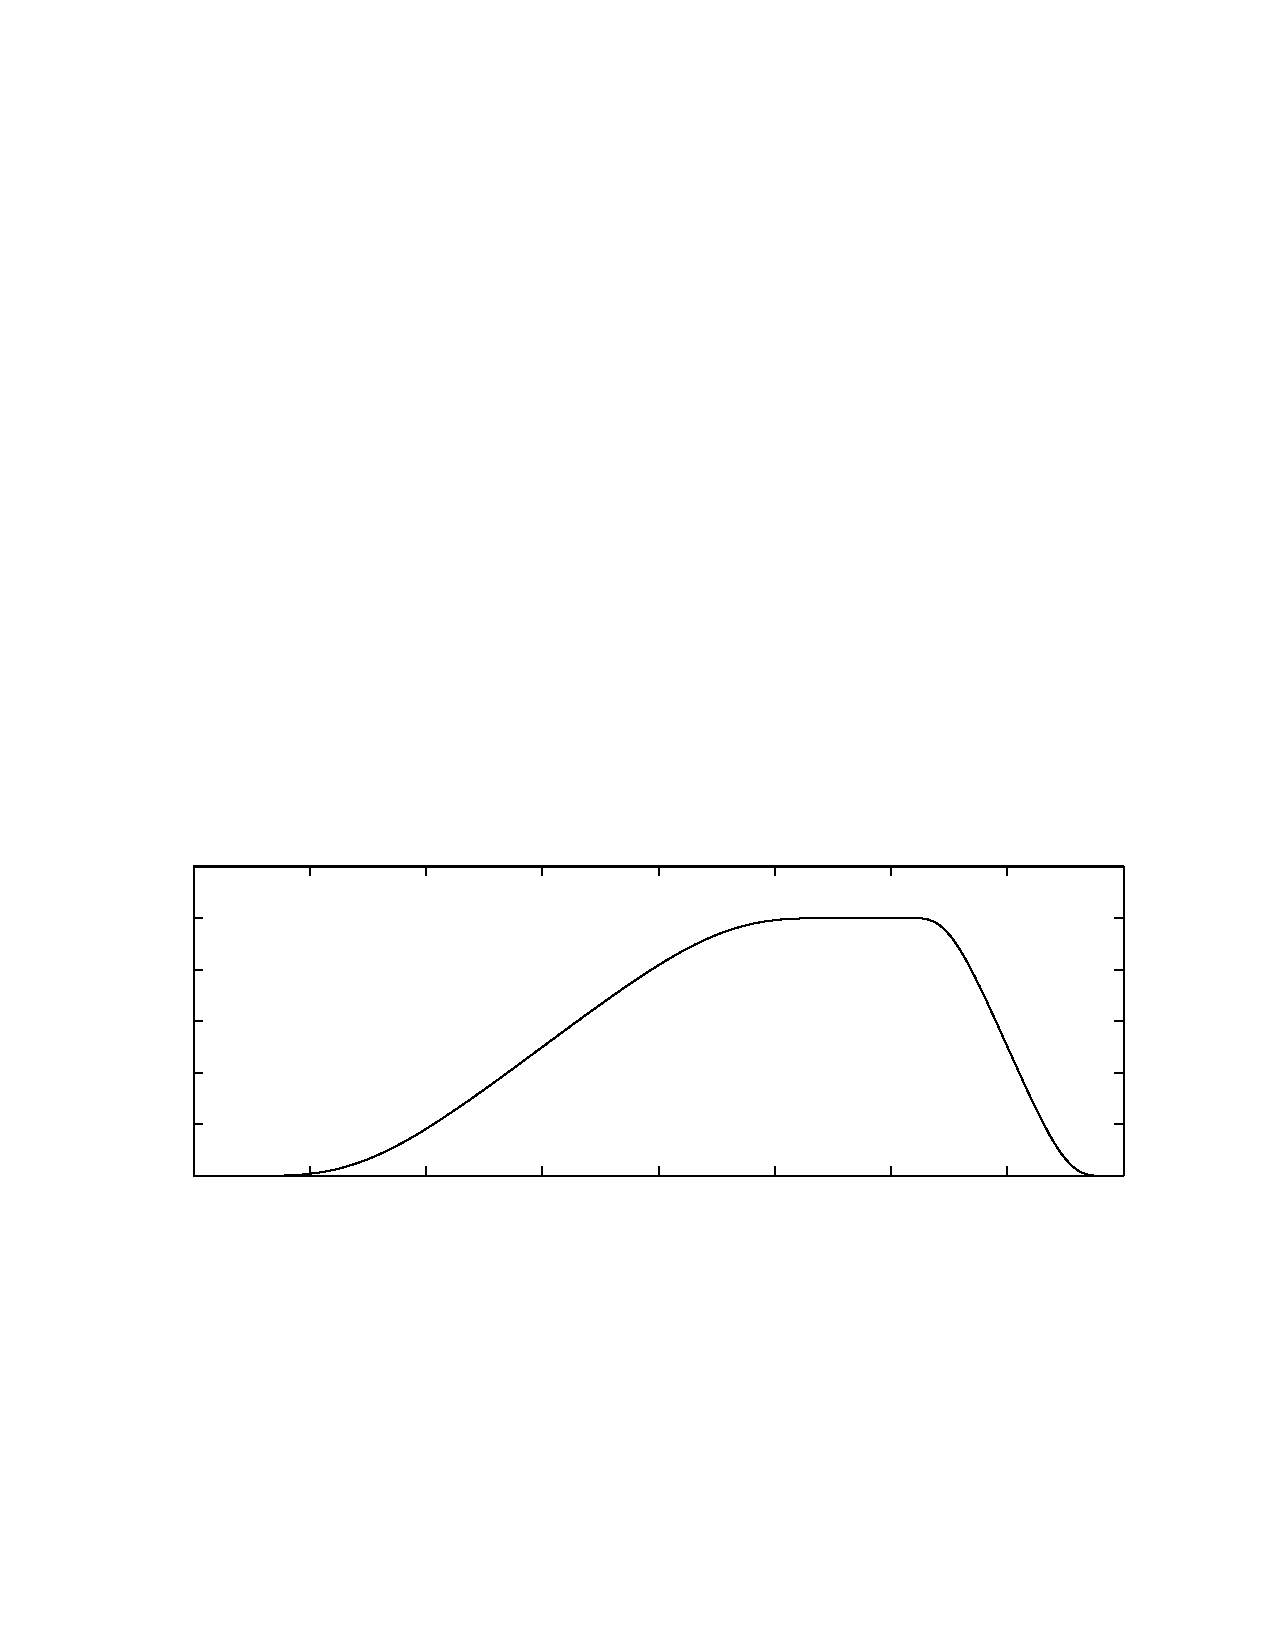
\includegraphics[width=0.65\textwidth]{frbi}
\put(-83,13){$\lambda$}
\put(-50,-7){rise}
\put(-67,-1){$\underbrace{\hbox{\hskip4.0cm}}$}
\put(-12,-7){fall}
\put(-15,-1){$\underbrace{\hbox{\hskip1.2cm}}$}
\caption{Schematic picture of the fringe region.  For this fringe the
sum of the rise and fall is the same as the total length.}
\label{fig:frbi}
\end{figure}

To achieve maximum damping both the total length of the fringe and
$\lambda_{\max}$ have to be tuned. The actual shape of $\lambda (x)$
is less important for the damping but it should have its maximum
closer to $x_{\text{end}}$ than to $x_{\text{start}}$. The damping is
also strongly influenced by the resolution of the disturbance that
should be damped.

In summary the main parameters determining the damping properties of
the fringe forcing are
\begin{itemize}
\item Length of fringe ($L$)
\item Strength of fringe ($\lambda$)
\item Shape of fringe
\item Resolution of simulation
\item Influence of blending (for boundary layer flows)
\end{itemize}
An investigation on how the fringe parameters effect the disturbance
in the fringe can be found in \cite{alundbladh:sberling:mskote:1999}
and example cases can be found in the \epath{examples}
directory. Generally however one usually has to try a few different
sets of fringe parameters when setting up a new flow case and make
sure that the critical disturbances are damped out satisfactory.

For maximum computational efficiency the simulated flow has to be
considered when the fringe parameters are tuned. Assuming that the
achieved damping is sufficient, a short fringe reduces the box length
and therefore the required CPU time per iteration. However, if the
flow gradients introduced in the fringe region are larger than those
in the physical domain that may decrease the time step and
consequently increase the necessary number of iterations. Note that
the boundary layer growth causes outflow through the free-stream
boundary. The streamwise periodicity requires that all that fluid
reenters in the fringe region.

Analysis of the Navier--Stokes equations with a fringe forcing term
yields an additional part of the disturbance associated with the
pressure with a decay independent of $\lambda$. For a boundary layer,
this solution decays appreciably over a downstream distance equal to
the boundary layer thickness, and thus the fringe region must be some
factor (say 10 to 30) times this thickness to get a large decay
factor, see \cite{Nordstrom-Nordin-Henningson}.


% ====================================================================
\section{Boundary conditions}\label{freebc}
% ====================================================================
The boundary conditions in the horizontal directions are periodic
which hold for all flows implemented. The wall-normal boundary
conditions however may differ between the different flow types;
additionally, inhomogeneous boundary conditions may be specified
(\emph{e.g.}\ wall blowing and suction).


% --------------------------------------------------------------------
\subsection{Poiseuille flow}
% --------------------------------------------------------------------
The natural no-slip boundary conditions on both walls, located at
$y=\pm 1$, read
\begin{equation}
v|_{\mathrm{wall}}=0\,,\quad \left.\frac{\partial v}{\partial y}\right|_{\mathrm{wall}}=0\,, \quad \omega|_{\mathrm{wall}}=0\,.
\label{eq:bcchannel}
\end{equation}

For disturbance generation and control by blowing and suction through
the wall, an arbitrary time dependent velocity distribution,
\begin{equation}
\begin{aligned}
v|_{y=1}  & = v_{\text{BS}_u}(x,z,t)\,,\\
v|_{y=-1} & = v_{\text{BS}_l}(x,z,t)\,,
\end{aligned}
\end{equation}
can be used. Several types of control signals are available.


% --------------------------------------------------------------------
\subsection{Couette flow} 
% --------------------------------------------------------------------
The boundary conditions for Couette flow impose constant streamwise
velocity, positive on the upper wall and negative on the lower wall,
and zero wall-normal and spanwise velocity components.


% --------------------------------------------------------------------
\subsection{Boundary layer flow}
% --------------------------------------------------------------------
The boundary conditions in the horizontal directions are periodic but
one needs to specify boundary conditions at the wall and in the
free-stream, to solve equations (\ref{eq:ph}) and (\ref{eq:om}).

For disturbance generation and control by blowing and suction through
the wall, an arbitrary time dependent velocity distribution,
\begin{equation}
v|_{y=0}=v_{\text{BS}}(x,z,t)\,,
\end{equation}
can be used.

The flow is assumed to extend to an infinite distance perpendicular to
the wall. However, the discretization discussed below can only handle
a finite domain. Therefore, the flow domain is truncated and an
artificial boundary condition is applied in the free-stream at a
wall-normal position $y_L$.

The Dirichlet boundary condition, defined as
\begin{equation}
\mathbf{u}_{y=y_L}=\boldsymbol{\mathcal{U}}_{y=y_L}\,,
\end{equation}
is the simplest one, where $\boldsymbol{\mathcal U}(x,y)$ is a base
flow that is normally chosen as a Falkner--Skan--Cooke (FSC) flow. An
arbitrary pressure gradient, to for instance create a separation
bubble, can be imposed by choosing $\boldsymbol{\mathcal U}$
accordingly.

The desired flow solution generally contains a disturbance and that
will be forced to zero by the Dirichlet condition. This introduces an
error compared to the exact solution for which the boundary condition
is applied at an infinite distance from the wall.  The error may
result in increased damping for disturbances in the boundary layer.

Some improvement can be achieved by using a Neumann condition,
\begin{equation}
\left.{\partial \mathbf{u} \over \partial y}\right|_{y=y_L}=\left.\frac{\partial \boldsymbol{{\mathcal U}}}{\partial y}\right|_{y=y_L}.
\end{equation}
This condition can be shown to be stable if there is outflow at the
boundary or the inflow is weaker than $O(1/\mathit{Re})$. This
restriction is usually fulfilled if the boundary is placed on a
sufficiently large distance from the wall, so that the disturbance
velocity is small.

A generalization of the boundary condition used by
\cite{Malik-Zang-Hussaini} allows the boundary to be placed closer to
the wall. It is an asymptotic condition that decreases the error
further and it reads
\begin{equation}
\left.\left({\partial \hat{\mathbf{u}} \over \partial y}+|k|\hat{\mathbf{u}}\right)\right|_{y=y_L}=
\left.\left(\frac{\partial \hat{\boldsymbol{\mathcal U}}}{\partial y}+|k|\hat{\boldsymbol{\mathcal U}}\right)\right|_{y=y_L},
\end{equation}
where $\hat{(\cdot)}$ denotes the horizontal Fourier transform with
respect to the horizontal coordinates, $k^2=\alpha^2+\beta^2$ and
$\alpha$ and $\beta$ are the horizontal wavenumbers (see equation
(\ref{eq:fout})).  Thus this condition is most easily applied in
Fourier space.  The boundary condition exactly represents a potential
flow solution decaying away from the wall. It is essentially
equivalent to requiring that the vorticity is zero at the boundary.
Thus, it can be applied immediately outside the vortical part of the
flow.


% --------------------------------------------------------------------
\subsection{Asymptotic suction boundary layer flow}
% --------------------------------------------------------------------
The asymptotic suction boundary layer (ASBL) is an analytical solution
to the Navier--Stokes equations when uniform wall-normal suction, with
velocity $-v^{}_s$, is applied at the wall. It can be written as
\begin{equation}
\mathbf{U}=(1-e^{-y},-v^{}_s,0)\,.
\end{equation}
The analytical solution allows the displacement thickness to be
calculated exactly, $\delta^*=\nu/v^*_s$ and the Reynolds number to be
expressed as the velocity ratio,
$\mathit{Re}_{\text{asbl}}=U^{}_\infty/v^*_s$, where $-v^*_s$ is the
dimensional suction velocity.

The constant suction requirement at the wall is removed by subtracting
the Navier--Stokes equations by $v^{}_s$ which gives the following
modified form of equation \ref{eq:hdef}
\begin{equation}
H_1=(v-v_s)\vartheta-w\omega\,,\quad H_3=u\omega-(v-v_s)\chi\,,
\end{equation}
where $(\chi,\omega,\vartheta)$ denotes the vorticity vector. Note that
no additional forcing is needed to keep the base flow parallel. More
details about the ASBL and its implementation in \esoft{Simson} can be
found in \cite{levin:114104}.


% --------------------------------------------------------------------
%\subsection{Wall jet boundary layer flow}
% --------------------------------------------------------------------


% --------------------------------------------------------------------
\subsection{Surface roughness}\label{sec:roughness}
% --------------------------------------------------------------------
The spectral framework of \esoft{bla} requires uniform boundaries.
Thus, roughness elements on the surface of the plate cannot be
included in terms of grid geometry, but they need to be modeled by
modified boundary conditions. A projection method is employed here, as
originally proposed in \cite{Choudhari-Streett} and
\cite{Crouch:loc_recept}. A Taylor expansion of fourth order is used
to project the no-slip conditions along the desired bump contour onto
the lowest grid plane $y=0$, where $y$ is the wall-normal coordinate,
\begin{equation}
v_i|_{y=0}\approx\underbrace{v_i(h)}_{\equiv 0}-\left.h\frac{\partial v_i}{\partial y}\right|_{y=0}-
\hspace{0.2cm}...\hspace{0.2cm}-\left.\frac{h^4}{4!}\frac{\partial^4 v_i}{\partial y^4}\right|_{y=0}
\hspace{0.2cm},\hspace{0.3cm}i=1,2,3
\label{eq:roughn-proj}
\end{equation}
where $h=h(x,z)$ denotes the contour function of the bump and $v_i$
can be either the base-flow profile or the instantaneous velocity. In
the present implementation the bump function $h$ is localized in the
chordwise direction $x$ (step function, equation
(\ref{eq:step-function})) and periodic along the span $z$. \par The
wall-normal velocity derivatives in equation (\ref{eq:roughn-proj})
are obtained from the base-flow profiles. The representation of the
no-slip conditions along the desired roughness contour can be improved
by updating the bump conditions regularly. Then, the velocity
derivatives of equation (\ref{eq:roughn-proj}) are taken from the
current flow field.


% --------------------------------------------------------------------
\subsection{Jet in crossflow}\label{sec:jet-in-crossflow}
% --------------------------------------------------------------------
To model a jet discharging normal to a crossflow either a top-hat jet
profile or a parabolic jet profile can be imposed. The former boundary
condition models fluid ejected from a turbulent pipe, whereas the
latter models a laminar pipe flow. The main parameters (set in
\efile{bla.f}) are the position of the jet orifice $(x_{\text{jet}},
z_{\text{jet}})$, the jet diameter $D_{\text{jet}}$ and the ratio
\begin{equation}
R_{\text{jet}}=\frac{\bar{v}_{j}}{U_\infty}
\end{equation}
of the bulk velocity $\bar{v}_j$ from the jet orifice to the cross-flow
velocity.

The first boundary condition is a top-hat profile given by,
\begin{equation}
v_j(r) = \frac{1}{2}[1-\tanh(5(r-1/r))]\,,
\end{equation}
where $r=2\sqrt{x^2+z^2}/(\alpha D_{\text{jet}})$. In this case, the
diameter of the jet is defined by the bulk velocity, by choosing
$\alpha=0.9919$ such that the bulk velocity equals the maximum
velocity, $\bar{v}_{j}=v_{j,\max}$. The second boundary condition is a
parabolic profile multiplied with a Gaussian function,
\begin{equation}
v_j(r) = (1-r^2)e^{(-(r/0.7)^4)}\,.
\end{equation}
For this boundary condition the relation between the bulk and the
maximum velocity is $\bar{v}_{j}\approx v_{j,\max}/3$.

Furthermore, for the actual implementation in the numerical code, the
net mass flux is set to zero via an artificial uniform suction applied
at the lower wall, \emph{i.e.}\ the ($(0,0)$-mode of the
$v$-component. This uniform suction velocity can however be subtracted
from the velocity fields and statistics.


% ====================================================================
\section{Initial conditions}\label{sec:baseflows}
% ====================================================================
To start a temporal or spatial simulation a laminar initial flow field
is required. For boundary layer flows it is constructed from
similarity solutions of the boundary layer equations and for
Poiseuille and Couette flows it can be given analytically.

In the boundary layer flow favorable and adverse pressure gradients
can be accounted for as well as the effect of a sweep. To obtain the
family of FSC similarity solutions it is assumed that the chordwise
outer-streamline velocity obeys the power law
$U_{\infty}^*=U_0^*(x^*/x_0^*)^m$ and that the spanwise velocity
$W_{\infty}^*$ is constant. Here $U_0^*$ is the free-stream velocity
at the beginning of the computational box and the asterisks $(*)$
denote dimensional quantities. Note that the Blasius profile is a
special case of FSC with zero cross flow component and pressure
gradient. If the similarity variable $\eta$ is chosen as
\begin{equation*}
\eta(y^*)=y^*\sqrt{\frac{m+1}{2}\frac{U_{\infty}^*}{2\nu x^*}}
\end{equation*}
one can derive the following self-similar boundary layer profiles,
\begin{equation*}
\begin{aligned}
f'''+ff'' & + \beta_h(1-f'^2) = 0\,,\\
g''& + fg' =0\,,
\end{aligned}
\end{equation*}
where the Hartree parameter $\beta_h$ relates to the power law
exponent $m$ as $\beta_h=2m/(m+1)$. The accompanying boundary
conditions are
\begin{equation*}
\begin{aligned}
f=f'=g=0\quad&\text{for}\quad\eta=0\,,\\
f'\rightarrow 1\,,\quad g\rightarrow 1 \quad &\text{as} \quad\eta\rightarrow \infty\,.
\end{aligned}
\end{equation*}
The complete derivation can be found in \emph{e.g.}\
\cite{schlichting:1979} and \cite{jcooke:1950}. From the FSC
similarity solutions, one constructs the nondimensional velocity
profiles
\begin{subequations}
\begin{align}
U(y) & = f'(\eta(y))\,,\label{eq:vel:prof:a}\\
W(y) & = \frac{W_{\infty}}{U_{\infty}}g(\eta(y))\,,\label{eq:vel:prof:b}
\end{align}
\end{subequations}
for a fixed $x$ and where $y=y^*/\delta^*$.  The velocity profiles
\eqref{eq:vel:prof:a} and \eqref{eq:vel:prof:b} are then used when
constructing the base flow.

The initial similarity solution for the passive scalar is found from
solving
\begin{equation*}
\theta''=-\mathit{Pr}\, f\, \theta' + \mathit{Pr}\, m_1(2-\beta_h) f' \theta \,,
\end{equation*}
subject to the boundary conditions
\begin{equation*}
\theta=1\quad \text{for}\quad\eta=0\,,\ \theta=0 \quad \text{as} \quad\eta\rightarrow \infty \,.
\end{equation*}
Here, $\mathit{Pr}$ is the Prandtl (or Schmidt) number, and $m_1$ is
the power-law exponent for the scalar distribution along the
streamwise direction. Note that $m_1=0$ defines a constant scalar
value at the wall (\emph{i.e.}\ $\theta=1$), whereas $m_1=1/2$ leads
to a similarity solution with constant wall-normal derivative
(\emph{i.e.}\ isoflux boundary condition).
\begin{table}[!h]
\begin{center}
\begin{tabular}{rl}
\hline
\hline
\texttt{Type} & Description\\ 
\hline
%  -3    & Temporal asymptotic suction BL\\
  $-2$  & Temporal Falkner--Skan--Cooke BL\\
  $-1$  & Temporal Falkner--Skan BL\\
   0    & No base flow (currently not in use)\\
   1    & Temporal Poiseuille\\
   2    & Temporal Couette\\
   3    & Temporal Blasius BL\\
   4    & Spatial Poiseuille\\
   5    & Spatial Couette\\
   6    & Spatial Blasius BL\\
   7    & Spatial Falkner--Skan BL\\
   8    & Spatial Falkner--Skan--Cooke BL\\
   9    & Parallel Blasius/Falkner--Skan/Falkner--Skan--Cooke BL with fringe\\
%  10    & Asymptotic suction BL with fringe\\
%  11    & Spatial wall jet BL\\
\hline
\hline
\end{tabular}
\end{center}
\caption{Available base flow types.}
\label{tab:flowtypes}
\end{table}


% ====================================================================
\section{Disturbance formulation and linearized solver}\label{sec:linearized:solver}
% ====================================================================
Introducing a decomposition of the flow variables into a base flow and
a disturbance part, $u_i=U_i+u_i'$ leads to an evolution equation for
$u_i'$ due to equation (\ref{eq:ns})
\begin{equation}
\begin{aligned}
{\partial u_i' \over \partial t} = & -{\partial p' \over \partial x_i} +
\epsilon_{ijk}(u_j'\omega_k'+U_j\omega_k'+u_j'W_k) \\
                                   & - {\partial \over \partial
x_i}\left({1\over 2}u_j' u_j'+U_ju_j'\right) + {1\over \mathit{Re}}\nabla^2 u_i'+F_i-G_i\,.
\end{aligned}
\label{eq:nsdist}
\end{equation}
Here, the rotation rate $\Omega_k$ is neglected; $W_k$ denotes the
vorticity field corresponding to the base flow $U_i$. The base flow is
assumed to satisfy the stationary Navier--Stokes equations,
\begin{equation}
0 = -{\partial P \over \partial x_i} +
\epsilon_{ijk}U_jW_k - {\partial \over \partial
x_i}\left({1\over 2}U_j U_j\right) + {1\over \mathit{Re}}\nabla^2 U_i+G_i\,.
\label{eq:nsmean}
\end{equation}
Additionally, both $U_i$ and $u_i'$ are supposed to satisfy the
continuity constraint. $G_i$ can be considered the residual of the
base flow when put into the Navier--Stokes equations (\ref{eq:ns}),
and it will include the fringe force $\lambda(\mathcal{U}_i-U_i)$ for
spatial simulations. It also includes additional (unknown)
contributions if the base flow does not satisfy the Navier--Stokes
equations, \emph{e.g.}\ when using the boundary-layer equations to
compute $U_i$. For simulations using the disturbance formulation it is
therefore suggested to always use a converged solution of the
Navier--Stokes equations (\emph{i.e.}\ the converged steady result of
a simulation) as a base flow.

For spatial simulations, the terms $F_i$ and $G_i$ are given by the
fringe forcing (\ref{eq:fringeforce}). Then,
$G_i=\lambda(\mathcal{U}_i-U_i)$ and $F_i=\lambda(\mathcal{U}_i-u_i)$
and thus the combined forcing is simply damping the disturbance
velocity to zero in the fringe region,
\begin{equation}
F_i-G_i = \lambda(x) u'_i \,.
\end{equation}
The linearized Navier--Stokes equations are obtained from equation
(\ref{eq:nsdist}) by neglecting the nonlinear terms $u_j'\omega_k'$
and $u_j' u_j'$.


% ====================================================================
\section{Pressure solver}\label{sec:pressure}
% ====================================================================
By expressing the Navier--Stokes equations in the form of equations
(\ref{eq:vv}) and (\ref{eq:om}), the pressure does not need to be
taken into account. However, it might be of interest to solve for this
quantity as well as the velocity components. The pressure can, for
example, be used for detecting regions of rapid motion in a turbulent
boundary layer.
  
The Poisson equation for the pressure, equation
(\ref{eq:pr}), can be written as
\begin{equation}
\nabla^2(p+E)={{\partial H_i}\over{\partial x_i}} \,,
\label{eq:po22}
\end{equation}
where $E={1\over2}u_i u_i$ and $H_i$ as defined in (\ref{eq:hdef}).
Note that the term $F_i$ does not contain any disturbances in the
fringe region for the spatial simulations and is zero for the temporal
boundary layer.  This equation has a similar form as the equations for
$\phi$, $v$ and $\omega$ and can thus be solved using the same
numerical routine.

The boundary conditions at the wall ($y=0$) and at the upper boundary
($y=y_L$) are derived from the normal component of the Navier--Stokes
equations.  The boundary condition with non-zero wall velocities
becomes
\begin{equation}
{{\partial }\over{\partial y}}(p+E) \bigg |_{y=0}=\left(
{1\over \mathit{Re}}\nabla^2 v+\epsilon_{ijk}u_j(\omega_k+2\Omega_k)-{{\partial v}\over{\partial t}} \right) \bigg |_{y=0} .
\label{eq:bc10}
\end{equation}

The term ${\partial v/\partial t}$ is included for the case of flow
control like blowing/suction from the wall and is approximated with
first-order backward differences. For a wall with zero velocities the
boundary condition becomes
\begin{equation}
{{\partial }\over{\partial y}}(p+E) \bigg |_{y=0}=
{1\over \mathit{Re}}{{\partial^2 v}\over{{\partial y}^2}} \bigg |_{y=0}.
\label{eq:bc100}
\end{equation}

At $y=y_L$, for boundary layer flows, the boundary condition becomes
\begin{equation}
{{\partial }\over{\partial y}}(p+E)\bigg |_{y=y_L}\!\!\!\!\!=\left(
{1\over \mathit{Re}}\nabla^2 v+\epsilon_{ijk}u_j(\omega_k+2\Omega_k)+\lambda(x) ({\mathcal V}-v)-
{{\partial v}\over{\partial t}}\right) \bigg |_{y=y_L}\!\!\!\!\!,
\label{eq:bc13}
\end{equation}
where $\lambda(x)$ is the fringe function described in section 
\ref{sec:spatfor}.

For wavenumber zero the boundary condition (\ref{eq:bc13}) is
automatically fulfilled if boundary condition (\ref{eq:bc10}) is
fulfilled. It is required by the compatibility condition
\begin{equation}
\int _0 ^{y_L} {{d H_2}\over{ d y}} dy=
{{\partial }\over{\partial y}}(p+E) |_{y=y_L}-
{{\partial }\over{\partial y}}(p+E) |_{y=0} \,,
\end{equation}
which comes from the integration of equation (\ref{eq:po22}).  A
second boundary condition for $p$ itself is needed at $y=0$ and this
is chosen to be $p=0$. The mean pressure at the wall cannot be
determined and $p=0$ at the wall is a reference pressure.  It is not
reasonable to choose $p=0$ at $y=y_L$ because the location of the
free-stream is arbitrary chosen for numerical purposes.

It might seem to be a better approach to rewrite equation
(\ref{eq:pr}) as
\begin{equation}
\nabla^2p=-{{\partial u_i}\over{\partial x_j}}
{{\partial u_j}\over{\partial x_i}}+
{{\partial}\over{\partial x_i}}(2\epsilon_{ijk}u_j \Omega_k)+
{{\partial F_i}\over{\partial x_i}} \,,
\label{eq:po2}
\end{equation}
and solve for the pressure directly. The solution to equation
(\ref{eq:po2}) turns out to be sensitive to the values of the
velocities at the upper boundary. When using different boundary
conditions for the velocities, the solutions are slightly different,
hence the pressure will be different. The sensitivity comes from the
fact that the derivation in the normal direction in Chebyshev space is
dependent on the coefficients in all the collocation points.  These
coefficients change when transforming back and forth to physical
space.  Thus the derivations must be, for consistency, performed at
the same time, with no transformations between them.  These problems
are avoided by solving for the pressure plus energy as in equation
(\ref{eq:po22}).

If turbulent statistics involving pressure are being calculated during
a simulation, the pressure is calculated in those time steps where the
sampling occurs.

Note that at the moment the pressure calculation is only possible if
the full Navier--Stokes equations are solved, \emph{i.e.}\ evaluating
the pressure in disturbance formulation (see previous section
\ref{sec:linearized:solver}) is not supported.


% ====================================================================
\section{Passive scalar}\label{sec:passive:scalar}
% ====================================================================
The equation to solve for a passive scalar is
\begin{equation}
\frac{\partial \theta}{\partial t} = -u_i\frac{\partial \theta}{\partial x_i} + \frac{1}{\mathit{Re}\, \mathit{Pr}} \nabla^2 \theta
\label{eq:theta}
\end{equation}
subject to appropriate boundary conditions. The molecular Prandtl
number (fluid dependent) is denoted $\mathit{Pr}$ and the combination
$\mathit{Pe}=\mathit{Re}\, \mathit{Pr}$ is the P\'eclet number. The
various terms in equation (\ref{eq:theta}) are advanced in time in a
similar manner as the corresponding terms in the Navier--Stokes
equations (see chapter \ref{chap:numerics}). Boundary conditions for
$\theta$ need to be given at both the lower wall and the upper
boundary (free-stream or wall).


% ====================================================================
\section{Selective frequency damping}\label{sec:selective:frequency}
% ====================================================================
The selective frequency damping method (SFD) can be used to obtain
steady solutions of the Navier--Stokes equations by time
marching. This is possible, even for unstable flow configurations, due
to an additional forcing term on the right-hand side which damps all
temporally fluctuating parts of the solutions. Further details are
given in
\cite{akervik_brandt_henningson_hoepffner_marxen_schlatter_2006}. The
forcing term reads
\begin{equation}
-\chi (u_i-\overline{u}_i) \,,
\label{eq:sfdforc}
\end{equation}
where $u_i$ is the velocity and $\overline{u}_i$ a corresponding
\emph{temporally} low-pass filtered flow field. The filtered field is
obtained using the differential form of an exponential filter leading
to an evolution equation
\begin{equation}
\frac{\partial \overline{u}_i}{\partial t} = \frac{u_i-\overline{u}_i}{\Delta} \ ,
\label{eq:sfdev}
\end{equation}
with the filter width $\Delta$. If SFD is enabled, the forcing term
(\ref{eq:sfdforc}) is explicitely added to the governing equations
(\ref{eq:ns}), and the evolution equation for the filtered solution
(\ref{eq:sfdev}) is solved via the same explicit Runge-Kutta scheme.


% ====================================================================
\section{Large-eddy simulation}\label{sec:LES}
% ====================================================================
In large-eddy simulation (LES), the \emph{filtered} Navier--Stokes
equations are solved. The application of the primary LES filter is
denoted by an overbar, \emph{i.e.}\ $\overline{u}_i$, $\overline{p}$
and $\overline{\theta}$ for the filtered velocities, pressure and
scalar, respectively. Note that this primary LES filter is usually the
implicit grid filter due to the lower resolution employed for LES
calculations. The governing equations for the resolved (filtered)
quantities read
\begin{equation}
\begin{aligned}
\frac{\partial \overline{u}_i}{\partial t} + \overline{u}_j\frac{\partial \overline{u}_i}{\partial x_j} & =  -\frac{\partial \overline{p}}{\partial x_i}+\frac{1}{\mathit{Re}} \frac{\partial^2 \overline{u}_i}{\partial x_j \partial x_j} - \frac{\partial \tau_{ij}}{\partial x_j} \,, \\
\frac{\partial \overline{u}_j}{\partial x_j} & = 0 \,, \\
\frac{\partial \overline{\theta}}{\partial t} + \overline{u}_j\frac{\partial \overline{\theta}}{\partial x_j} & = \frac{1}{\mathit{Re}\, \mathit{Pr}} \nabla^2 \overline{\theta} - \frac{\partial q_j}{\partial x_j} \,.
\end{aligned}
\end{equation}
The unclosed subgrid-scale (SGS) stresses and scalar flux are
\begin{equation}
\begin{aligned}
\tau_{ij} & = \overline{u_iu_j} -\overline{u}_i\,\overline{u}_j \,, \\
q_j       & = \overline{u_j \theta} - \overline{u}_j \overline{\theta} \,.
\end{aligned}
\end{equation}


% --------------------------------------------------------------------
\subsection{Dynamic Smagorinsky model}
% --------------------------------------------------------------------
The eddy-viscosity ansatz due to Boussinesq relates the deviatoric
part of the SGS stresses to the resolved strain rate,
\begin{equation}
\tau_{ij} - \frac{\delta_{ij}}{3}\tau_{kk} = 
\tau_{ij}^* = -2 \nu_t \overline{S}_{ij} \,,
\end{equation}
with the strain rate
\begin{equation}
\overline{S}_{ij} = \frac{1}{2}
\left(\frac{\partial \overline{u}_i}{\partial x_j} + 
      \frac{\partial \overline{u}_j}{\partial x_i}\right) \,.
\end{equation}
Within the eddy-diffusivity ansatz, the scalar flux is approximated as
being proportional to the mean scalar gradient,
\begin{equation}
q_j=-k_t \frac{\partial \overline{\theta}}{\partial x_j}
\end{equation}
with $k_t=\nu_t / \mathit{Pr}_t$. The turbulent Prandtl number
$\mathit{Pr}_t$ is approximately a constant of order one. A standard
value is $\mathit{Pr}_t = 0.6$.

The Smagorinsky model \citep{smagorinsky_1963} gives the eddy
viscosity as follows
\begin{equation}
\nu_t=C \Delta^2 |\overline{S}|\ \ \text{with} \ |\overline{S}|=
(2\overline{S}_{ij}\overline{S}_{ij})^{1/2} \,.
\end{equation}
The model coefficient $C=C_S^2$ can be determined dynamically using
the well-known dynamic procedure
\citep{germano_piomelli_moin_cabot_1991,lilly_1992}. Commonly, a
two-dimensional spectral cutoff filter at $\omega_c=\pi/2$ acting in
the wall-parallel directions is employed as a test filter. The
coefficient $C$ predicted by the dynamic procedure is known to
fluctuate strongly in both space and time. Therefore, in the present
implementation, a spanwise averaging is performed, \emph{i.e.}\
$C=C(x,y,t)$.  Additionally, a clipping can be employed, either
requiring a positive model coefficient $C=\max(C,0)$, or positive
total viscosity $\nu_t=\max(\nu_t,-\nu)$. As common practice, the LES
computations are performed on the coarse (\emph{i.e.}\ non-dealiasing)
grid.


% --------------------------------------------------------------------
\subsection{High-pass filtered Smagorinsky model}
% --------------------------------------------------------------------
Recent developments in LES have shown that computing the SGS model
forces based on the small-scale fluctuations of the flow alone can be
very successful and lead to accurate results. This idea was first put
forward in the variational multiscale (VMS) approach, where a
separation between large and small scales is performed using
hierarchical basis function and the modeling is restricted to only the
small scales. A physical-space formulation of the VMS method using
spatial filters was used in \cite{stolz_schlatter_kleiser_2005}. The
high-pass filtered (HPF) eddy-viscosity model, using a high-pass
filter $H$, is written as
\begin{equation}
\tau_{ij}-\frac{1}{3}\tau_{kk}\delta_{ij} = 
2\nu_t^\mathrm{HPF} S_{ij}(H*\overline{u}) \,,
\label{eq:hpf_ev}
\end{equation}
with both $S_{ij}(H*\overline{u})$ and the eddy viscosity computed
from the high-pass filtered velocity,
\begin{equation}
\nu_t^\mathrm{HPF} = 
C \overline{\Delta}^2|S(H*\overline{u})| \,.
\label{eq:hpf_smag}
\end{equation}
The symbol $*$ stands for convolution in physical space. This model is
denoted as small-``small'' since the eddy viscosity
$\nu_t^\mathrm{HPF}$ is computed from the small scales, and is applied
to the Navier--Stokes equation using the small-scale strain rate. Due
to nonlinearity, however, the model influence (\ref{eq:hpf_ev}) is not
restricted to the small part of the governing equations.

A consistent dynamic procedure for the HPF model (\ref{eq:hpf_ev}),
(\ref{eq:hpf_smag}) has been introduced in \cite{bruhn_2006}.
Essentially, one can follow a similar way as in the procedure by
\cite{germano_piomelli_moin_cabot_1991}, however, the residual
stresses are now taken from their respective HPF formulation.

The high-pass filters employed are based on the filter $G$ defined in
\cite{stolz_adams_kleiser_2001a}. The filter definition for
non-equidistant grids, \emph{e.g.}\ in the wall-normal direction,
assures that all moments in physical space up to second order are
vanishing.  The cutoff wavenumber $\omega_c$ is defined by
$\hat{G}(\omega_c)=1/2$ with the hat indicating a Fourier transform
(transfer function).  Usually, $\omega_c=2\pi/3$ is a preferred
value. Based on $G$, related high-pass filters can readily be
constructed by $H_N = (I-G)^{N+1}$.  The three-dimensional filters are
derived from the one-dimensional filters by a tensor product. $H_N$ is
at least of order $r(N+1)$ with $r$ being the order of $G$. The latter
is at least $r=3$ on non-equidistant grids.


% --------------------------------------------------------------------
\subsection{Relaxation-term model (ADM-RT)}
% --------------------------------------------------------------------
Whereas the Smagorinsky model is based on the eddy-viscosity
assumption, the ADM-RT model acts on the velocity components directly.
The model employs the relaxation term used in the context of the
approximate deconvolution model (ADM)
\citep{stolz_adams_kleiser_2001a}. It has been shown in \emph{e.g.}\
\cite{schlatter_2005} that for spectral simulations the deconvolution
operation applied in the ADM approach is not necessary. Therefore, the
SGS force due to the ADM-RT model is given by
\citep{schlatter_stolz_kleiser_2004}
\begin{equation}
\frac{\partial {\tau_{ij}}}{\partial x_j}  = \chi H_{N}*\overline{u}_i \,.
\end{equation}
$\chi$ is the model coefficient which can be set to a constant value
herein motivated by previous studies showing little dependency of the
results on the actual value of the coefficient (see \emph{e.g.}\
\cite{schlatter_2005}).  A good guess for the model coefficient can be
obtained by relating it to the time step of the integration, \emph{i.e.}\
$\chi \propto 1/\Delta t$, which itself is related to a physically
meaningful quantity (advection of small scales) by the CFL stability
condition.

The relaxation term $\chi H_{N}*\overline{u}_i$ is proportional to the
small-scale velocity fluctuations in the flow field. Therefore, it
will damp out these oscillations leading to a drain of kinetic energy
from the smallest resolved scales. It can be shown that the relaxation
term has a similar effect as an explicit filtering of the solution
every $(\chi \Delta t)^{-1}$ time steps.

The ADM-RT model proved to be accurate and robust in predicting
transitional and turbulent incompressible flows with spectral methods
\citep{schlatter_stolz_kleiser_2004,schlatter_2005}. Note that the
relaxation-term model is related to the spectral vanishing viscosity
approach. Due to the high-order filter $H_N$ with a cutoff frequency
of $\omega_c\approx 0.86\pi$ only the smallest represented eddies are
affected, whereas the larger, energy-carrying scales are not directly
influenced by the model contributions.

Similar to the HPF model, a dynamic procedure for the model
coefficient $\chi$ has been proposed in \cite{bruhn_2006}.


% ====================================================================
\section{Magneto-Hydrodynamics (MHD)}\label{sec:MHD} 
% ====================================================================
In the limit of low magnetic Reynolds number ($\mathit{Re}_{m} \ll~1$),
\cite{moreau_1998}, the induced magnetic field is very small when
compared to an externally imposed magnetic field $\mathbf{B_0}$,
and the electric current $\mathbf{J}$ is then given by the Ohm's law,
%
\begin{equation}
\mathbf{J}=\sigma\ \left(-\mathbf{\nabla}\Phi +\mathbf{u} \times
\mathbf{B_0}\right),
\end{equation}
%
where $\sigma$ is the electrical conductivity, $\Phi$ the electric
potential, $(E=-\mathbf{\nabla}\Phi)$, $E$ is the electric field, and
$\mathbf{u}$ is the velocity field. Using a characteristic magnetic
field $B$ the relevant non-dimensional quantities are
$\mathbf{b_0}=\mathbf{B_0}/B$, $\mathbf{j}=\mathbf{J}/(\sigma U B)$
and $\phi=\Phi\ \delta^*/(U B)$, with the velocity scale $U$. Then, the
following equations for an electrically conducting incompressible
fluid in the limit of $\mathit{Re}_{m}\ll 1$ are obtained:
%
\begin{equation}\label{momlrm}
\frac{\partial\mathbf{u}}{\partial t}+(\mathbf{u}\cdot
\mathbf{\nabla})\mathbf{u}=-\mathbf{\nabla}p+\frac{1}{\mathit{Re}}\nabla^2
\mathbf{u}+N\ (\mathbf{j}\times\mathbf{b_0})\,,
\end{equation}
\begin{equation}\label{currohms}
\mathbf{j}=-\mathbf{\nabla}\phi+\mathbf{u}\times\mathbf{b_0}\,,
\end{equation}
\begin{equation}\label{maglrm}
\mathbf{\nabla}^2\phi=\mathbf{\nabla} \cdot (\mathbf{u}\times
\mathbf{b_0})=\mathbf{b_0}\cdot\mathbf{\omega}\,,
\end{equation}
%
where Eq.~(\ref{maglrm}) is a consequence of $\mathbf{\nabla} \cdot
\mathbf{j} = 0$ and is obtained by taking the divergence of
Eq.~(\ref{currohms}). Here $\mathbf{\omega}=\nabla\times\mathbf{u}$,
$p$ the dimensionless pressure and $\mathit{Re} = U \delta^*/\nu$ is
the hydrodynamic Reynolds number. Moreover, incompressibility imposes
$\mathbf{\nabla} \cdot \mathbf{u} = 0$.

The traditional choice $B=|\mathbf{B_{0}}|$ has been adopted for the
characteristic magnetic field so that $\mathbf{b_{0}}$ is a unit
vector in the direction of the magnetic field. The Stuart number (or
interaction parameter), $N=\sigma B^2 \delta^* / \rho U$, is the ratio
of the electromagnetic force to the inertial force and it is related
to the Hartmann number by $\mathit{Ha} = \sqrt{\mathit{Re}\, N} (= B
\delta^* \sqrt{\sigma /\rho \nu})$ where $\rho$ is the density.
Equations~(\ref{momlrm})--(\ref{maglrm}) are referred to as the
low-$\mathit{Re}_m$ MHD equations.

At present, in channel geometry the walls are assumed to be
non-conducting. Therefore, the boundary conditions for the current
density and the electrical potential are
%
\begin{equation}\label{bc1}
\left.j_{y}\right|_{\textrm{wall}}=-\left.\frac{\partial\phi}{\partial
y }\right|_{\textrm{wall}}=0\,,
\end{equation}
%
where $j_y$ is the wall-normal component of the current density.


% ====================================================================
%\section{Linear feedback control and estimation}\label{sec:linear:feedback}
% ====================================================================
%The linear optimal control package implemented in the code consists of
%two parts. The first part is a control algorithm that is based on full
%flow state information which is used together with precomputed control
%kernels which need to be supplied by the user. The second part is the
%estimator which uses precomputed estimation kernels and wall
%measurements to reconstruct an approximative flow state. The
%controller can thus be run in two different modes; either based on
%full state information (which is possible in a computer simulation but
%is less applicable in real application) or on the estimated state. The
%combined estimator and controller is called a compensator.

%The kernels can be chosen in many different ways but from linear
%control theory it s possible to derive linear optimal kernels. All the
%details about the theory and on how to solve the optimization problems
%in order to compute the control and estimation kernels can be found
%in, for example, \cite{mhogberg:dhenningson},
%\cite{jhoepffner:mchevalier:2003}, \cite{mattiasestimation} and
%\cite{chevalier:hoepffner:akervik:henningson:2007}. More details can
%also be found in \cite[see \emph{e.g.}][p. 463--470]{lewisbook}.

%The file formats for the kernels can be found in sections
%\ref{sec:lqr} and \ref{sec:lqg}.


% --------------------------------------------------------------------
%\subsection{Measurements}\label{sec:measurements}
% --------------------------------------------------------------------
%For the estimation problem one can choose between different wall
%measurements. The available measurements are the streamwise and
%spanwise shear stresses, wall pressure fluctuations, wall-normal
%derivative of the wall-normal vorticity and the second wall-normal
%derivative of the wall-normal velocity, defined as
%\begin{equation}
%%\left\{
%\begin{aligned}
%\tau_x   & = \tau_{xy} |_{\text{wall}} = \frac{1}{\mathit{Re}} \left.\frac{\partial u}{\partial y}\right|_{\text{wall}} = \frac{1}{\mathit{Re}}\frac{i}{k^2} ( \alpha D^2 v - \beta D \omega)|_\text{wall}\,,  \\
%\tau_z   & = \tau_{zy} |_{\text{wall}} = \frac{1}{\mathit{Re}} \left.\frac{\partial w}{\partial y}\right|_{\text{wall}} = \frac{1}{\mathit{Re}}\frac{i}{k^2} ( \beta D^2 v + \alpha D \omega)|_\text{wall}\,,  \\
%p                      & = p |_\text{wall} = \frac{1}{\mathit{Re}}\frac{1}{k^2} D^3 v|_{\text{wall}}\,, \\
%\omega_y & = \frac{1}{\mathit{Re}} D\omega|_{\text{wall}}\,, \\
%v_{yy}   & = \frac{1}{\mathit{Re}} D^2 v|_{\text{wall}}\,.
%\end{aligned}
%%\right.
%\label{measurementdef}
%\end{equation}
%Note that for the channel and Couette flow cases we measure the flow
%both at the upper and lower walls.


% --------------------------------------------------------------------
%\subsection{Extension to spatially developing flows}\label{sec:extension}
% --------------------------------------------------------------------
%When solving the linear control problem and computing optimal control
%and estimation gains we have linearized about a specific mean flow
%profile. When the gains are applied in the control and measurement
%strip, the mean flow varies along those regions \emph{i.e.}\ errors will be
%introduced due to the changes of the mean flow.  Based on findings in
%\cite{mhogberg:dhenningson}, \cite{markus:relaminarization:2003},
%\cite{mhogberg:mchevalier:dhenningson:2003}, and
%\cite{mattiasestimation} it was expected that the controller and the
%estimator had some robustness properties with respect to changes in
%the mean flow profile. Due to the fact that the convolution kernels
%themselves, for proper choices of parameters, are localized indicates
%that only local information is needed which relaxes the requirement of
%constant mean flow profile. Examples of control and estimation
%convolution kernels can be found in the references given above.


% ####################################################################
\chapter{Numerical method}\label{chap:numerics}
% ####################################################################
The temporal and spatial discretizations are described in detail in
the following sections.


% ====================================================================
\section{Temporal discretization}
% ====================================================================
The time advancement is carried out by one out of two semi-implicit
schemes. We illustrate them on the equation
\begin{equation}
{\partial \psi \over \partial t} = G + L\psi\,,
\label{eq:psi} 
\end{equation}
which is of the same form as equation (\ref{eq:ph}) and (\ref{eq:om}).
Here $\psi$ represents $\phi$ or $\omega$, $G$ contains the
(non-linear) advective, rotation and forcing terms and depends on all
velocity and vorticity components. Operator $L$ represents the
(linear) diffusion and is discretized implicitly using the second
order accurate Crank--Nicolson (CN) scheme. Operator $G$ is
discretized explicitly by a low storage third order three or four
stage Runge--Kutta (RK3) scheme.  These time discretizations may be
written in the following manner
\begin{equation}
\psi^{n+1} = \psi^n + a_n G^n + b_n
G^{n-1} + (a_n + b_n) \left({L\psi^{n+1} +
L\psi^n \over 2}\right),
\label{eq:ab2}
\end{equation}
where the constants $a_n$ and $b_n$ are chosen according to the
explicit scheme used and $G$ and $L$ are assumed to have no explicit
dependence on time. The two possibilities for the RK3 schemes are
shown in the table \ref{table1}.  Note that the schemes have three or
four stages which imply that a full physical time step is only
achieved every three or four iterations. The time used for the
intermediate stages are given by $t=t+c_n$, where $c_n$ is given in
table \ref{table1}.
\begin{table}
\begin{center}
\begin{tabular}{lccc}
\hline
\hline
        & $a_n/\Delta t^n$ & $b_n/\Delta t^n$ & $c_n/\Delta t^n$ \\ 
\hline
RK3     & 8/15  &  0       & 0\\
3-stage & 5/12  & $-17/60$ & 8/15\\
        & 3/4   & $-5/12$  & 2/3\\
\hline
RK3     & 8/17  &     0    & 0\\
4-stage & 17/60 & $-15/68$ & 8/17\\
        & 5/12  & $-17/60$ & 8/15\\
        & 3/4   & $-5/12$  & 2/3\\
\hline
\hline
\end{tabular}
\end{center}
\caption{Time stepping coefficients.}
\label{table1}
\end{table}

To obtain some insight into the properties of these discretizations
they will be applied to the two dimensional linearized Burgers'
equation with a system rotation. The eigenvalue analysis yields a
necessary condition for stability which must be augmented by an
experimental verification.  Putting the equation into the form of
equation~(\ref{eq:psi}) yields
\begin{equation}
\begin{aligned}
\psi & = { \left[ \begin{array}{c} u \\ w \end{array} \right] }\,, \\
G    & = {  \left[ \begin{array}{cc}
u_0 \partial / \partial x + w_0 \partial / \partial z & 2\Omega\\
-2\Omega & u_0 \partial / \partial x + w_0 \partial / \partial z 
\end{array} \right] \left[ \begin{array}{c} u \\ w \end{array} \right] }\,, \\
L    & = {1 \over \mathit{Re}} { \left[ \begin{array}{cc} 
\partial^2 / \partial x^2 + \partial^2 / \partial z^2 & 0  \\
0 & \partial^2 / \partial x^2 + \partial^2 / \partial z^2  \\ 
\end{array} \right]}\,,
\end{aligned}
\label{eq:burger2d}
\end{equation}
where $u_0$ and $w_0$ represent the flow field around which the
linearization was made.  System ~(\ref{eq:burger2d}) can be seen as an
approximation to equation~(\ref{eq:ns}).  The dependence of $\psi$ on
both the streamwise and spanwise coordinate directions have been
included in order to indicate how multiple dimensions enter into the
stability considerations.

We will for simplicity use Fourier discretization in the spatial
directions.  The Chebyshev method acts locally as a transformed
Fourier method and thus the stability properties derived here can be
applied with the local space step.  An exception to this occurs at the
end points where the transformation is singular.  It can be shown that
the Chebyshev method is more stable there. A numerical study of a
one-dimensional advection equation using the Chebyshev discretization
yields that the upper limit of its spectrum along the imaginary axis
is about 16 times lower than the simple application of the results
from the Fourier method.  This allows a corresponding increase of the
time step when the stability is limited by the wall-normal velocity at
the free-stream boundary.

Fourier transforming in $x$- and $z$-directions yields
\begin{equation}
\hat{\psi}_t = { \left[ \begin{array} {cc}
i\alpha u_0 + i\beta w_0 & 2\Omega\\
-2\Omega & i\alpha u_0 + i\beta w_0 
\end{array} \right] } \hat{\psi} - {\alpha^2 + \beta^2
\over \mathit{Re}}\hat{\psi}\,,
\label{eq:bur}
\end{equation}
where $\alpha$ and $\beta$ are the wavenumbers in the $x$- and
$z$-directions, respectively.  This equation can be diagonalized to
give the equation,
\begin{equation}
\hat{u}_t = i(\alpha u_0 + \beta w_0 \pm 2\Omega)\hat{u}
+ {\alpha^2 + \beta^2 \over \mathit{Re}}\hat{u}\,.
\label{eq:bur2}
\end{equation}

We assume that the absolute stability limit will first be reached for
the largest wavenumbers of the discretization $\alpha_{\text{max}}$ and
$\beta_{\text{max}}$, which corresponds to a wavelength of $2 \Delta x$
and $2 \Delta z$, respectively, where $\Delta x$ and $\Delta z$ are
the discretization step lengths in physical space. The following
parameters are useful for our analysis,
\begin{equation}
\begin{aligned}
\mu     & =  \Delta t (2|\Omega_k|+(\alpha_{\text{max}}| u_0 |+ \beta_{\text{max}}|w_0|)) \\
        & =  \Delta t \left( 2|\Omega_k|+\pi\left( {|u_0| \over \Delta x}  +
                     {|w_0| \over \Delta z} \right)\right), \\
\lambda & = {1 \over \mathit{Re}}\Delta t (\alpha^2_{\text{max}} + \beta^2_{\text{max}}) \\
        & = {1 \over \mathit{Re}}\pi^2\Delta t \left( {1 \over \Delta x^2} + {1 \over \Delta z^2} \right).
\end{aligned}
\label{eq:mu-lam}
\end{equation}
The parameter $\mu$ is usually called the spectral CFL number, in
analogy with the stability theory for finite difference equations.
Henceforth it will be termed simply the CFL number. Using the RK3--CN
time discretization we have the following three stages in each time
step for the model equation~(\ref{eq:bur2}),
\begin{equation}
\begin{aligned}
\hat{u}^{n+1} & = \hat{u}^n + i\mu a_1\hat{u}^n
-{\lambda \over 2}a_1(\hat{u}^{n+1} + \hat{u}^n)\,,\\
\hat{u}^{n+2} & = \hat{u}^{n+1} + i\mu (a_2\hat{u}^{n+1} + b_2\hat{u}^n)
-{\lambda \over 2}(a_2+b_2)(\hat{u}^{n+2} + \hat{u}^{n+1})\,,\\
\hat{u}^{n+3} & = \hat{u}^{n+2} + i\mu (a_3\hat{u}^{n+2} + b_3\hat{u}^{n+1})
-{\lambda \over 2}(a_3+b_3)(\hat{u}^{n+3} + \hat{u}^{n+2})\,.
\end{aligned}
\label{eq:mrk3}
\end{equation}
\begin{figure}[tb]
\setlength{\unitlength}{1mm}
\centering
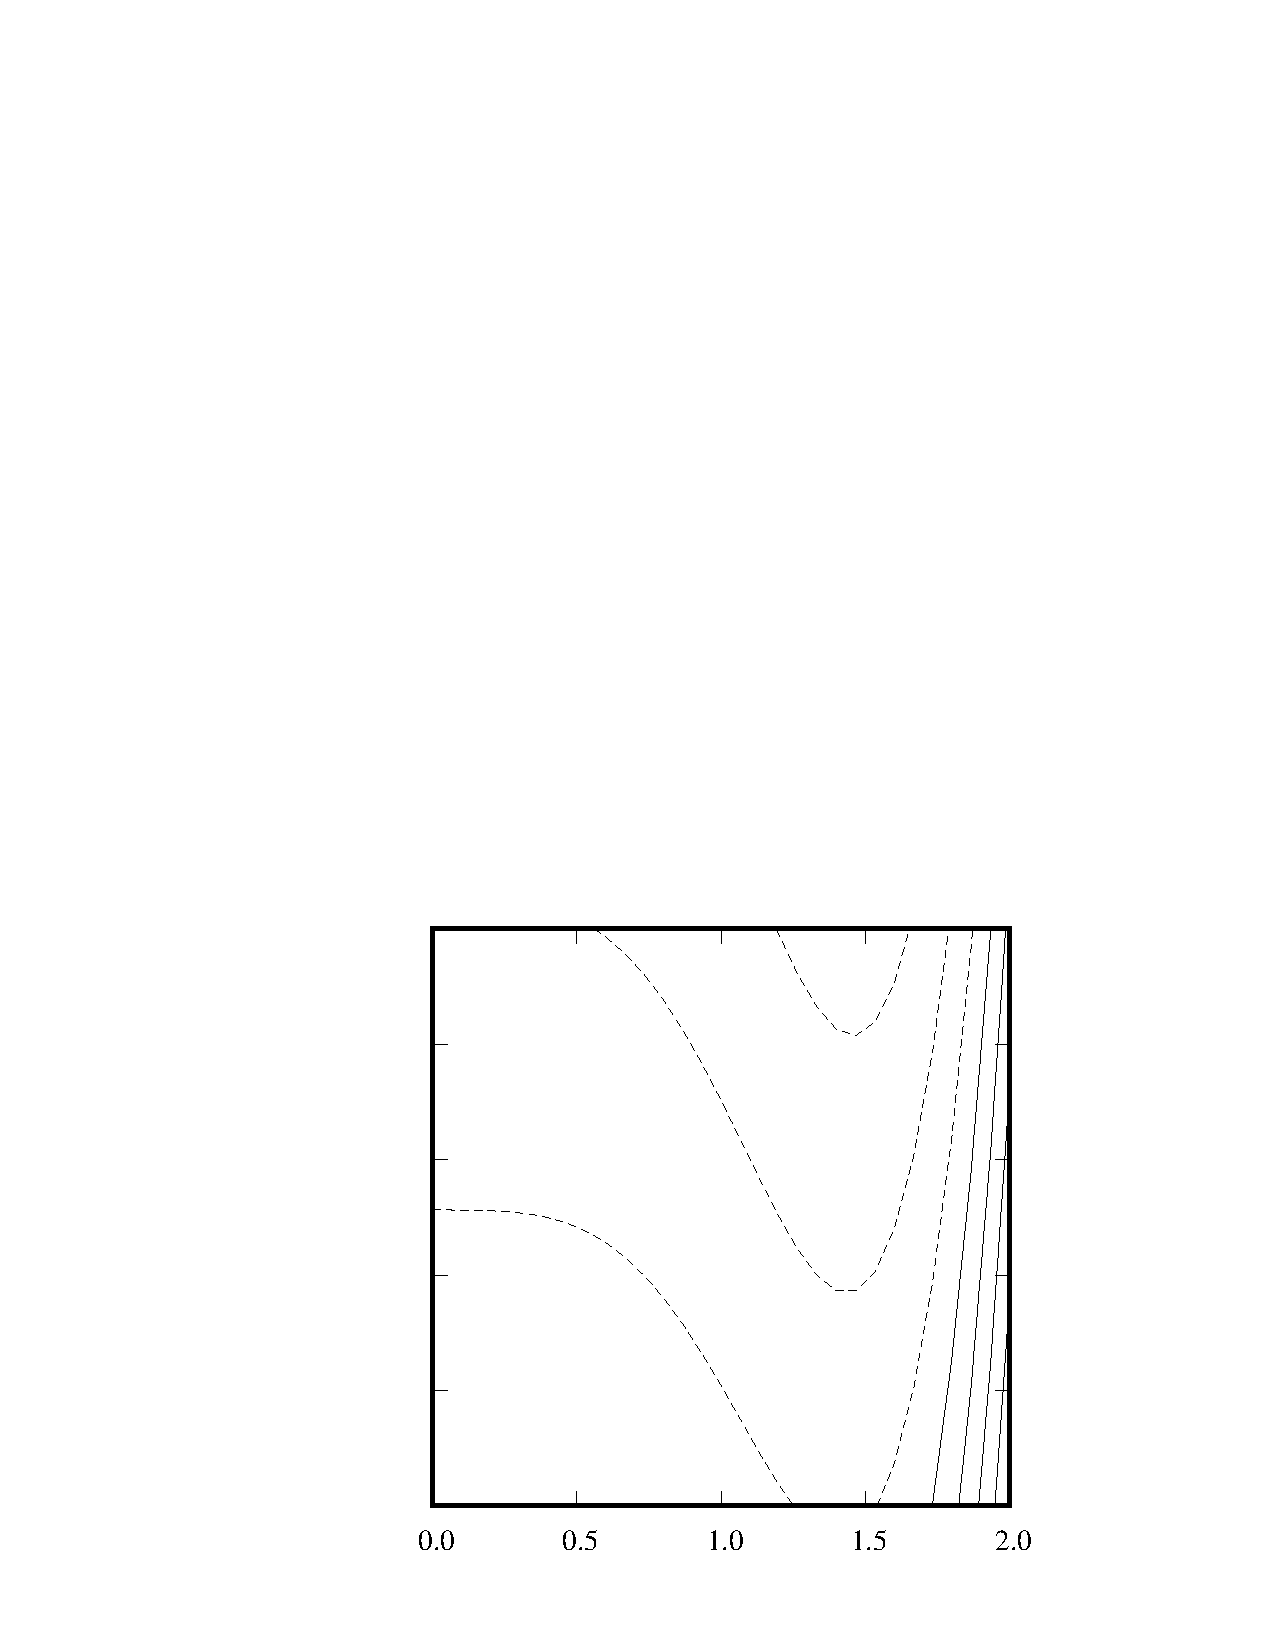
\includegraphics[width=0.45\textwidth]{rk3cn}
\put(-56,29){$\lambda$}
\put(-27,-3){$\mu$}
\caption{Contours of constant amplification factor for
the RK3-CN method. Contour spacing is 0.05 with dashed
lines indicating that the amplification factor is below unity.}
\label{fig:sta}
\end{figure} 

The absolute stability regions, \emph{i.e.}\ the regions where all
solutions to the above difference equations are bounded in the $\mu$
-- $\lambda$ plane, can now be found by calculating the roots of the
associated characteristic polynomials. Contours of constant absolute
values of the roots, for the RK3-CN method, are given in figure
\ref{fig:sta}. Note that higher values of $\lambda$ (lower Reynolds
number) stabilizes the method, \emph{i.e.}\ increases the CFL number
$\mu$ that is allowed for an absolutely stable solution. In the limit
of infinite Reynolds number the RK3-CN method approaches the limit
$\sqrt 3$, a result which also can be arrived at through the standard
analysis of the RK3 scheme alone.  The analysis for the four stage
method is analogous and the stability limit is $\sqrt 8$.

If the time advancement scheme~(\ref{eq:ab2}) is applied to
equations~(\ref{eq:ph}) and~(\ref{eq:om}) we find (for the moment
disregarding the boundary conditions),
\begin{equation}
\begin{aligned}
\left(1-{a_n+b_n\over 2\mathit{Re}}\nabla^2\right)\phi^{n+1} & = \left(1+{a_n+b_n\over
2\mathit{Re}}\nabla^2\right)\phi^n + a_nh_v^n + b_nh_v^{n-1}\,, \\
\nabla^2v^{n+1} & = \phi^{n+1}\,,
\end{aligned}
\label{eq:tph} 
\end{equation}
and
\begin{equation}
\begin{aligned}
\left(1-{a_n+b_n\over 2\mathit{Re}}\nabla^2\right)\omega^{n+1} & = \left(1+{a_n+b_n\over
2\mathit{Re}}\nabla^2\right)\omega^n + a_nh_{\omega}^n + b_nh_{\omega}^{n-1}\,.
\end{aligned}
\label{eq:tom}
\end{equation}


% ====================================================================
\section{Horizontal discretization -- Fourier expansions}
% ====================================================================
The discretization in the horizontal directions uses a Fourier series
expansion which assumes that the solution is periodic.

The streamwise and spanwise dependence of each variable can then be
written
\begin{equation}
u(x,z) =
\sum_{l=-({N_x\over 2}-1)}^{{N_x\over 2}-1}
\sum_{m=-({N_z\over 2}-1)}^{{N_z\over 2}-1}\hat{u}(\alpha_l
,\beta_m)e^{(i({\alpha_{l}x + \beta_{m}z}))}\,,
\label{eq:fout} 
\end{equation}
where $\alpha_{l}=2\pi l/x_L$ and $\beta_{m}=2\pi m/z_L$, and $N_x$
and $N_z$ are the number of Fourier modes included in the respective
directions.  Note that the indices on the discrete wavenumbers
$\alpha$ and $\beta$ are sometimes left out for notational convenience
and that $k^2=\alpha^2+\beta^2$.


% --------------------------------------------------------------------
\subsection{Normal velocity and normal vorticity equations}
% --------------------------------------------------------------------
Expanding the dependent variables of equation~(\ref{eq:tph}) in
Fourier series gives
\begin{equation}
\begin{aligned}
\left(1-{a_n+b_n\over 2\mathit{Re}}(D^2-k^2)\right)\hat{\phi}^{n+1} & = \left(1+{a_n+b_n\over
2\mathit{Re}}(D^2-k^2)\right)\hat{\phi}^n \\
 &\quad  + a_n\hat{h}_v^n + b_n\hat{h}_v^{n-1}\,, \\
(D^2-k^2)\hat{v}^{n+1} & = \hat{\phi}^{n+1}\,,
\end{aligned}
\label{eq:ftph} 
\end{equation}
where $D$ signifies a derivative in the normal direction. Note that
the above equations are two linear constant coefficient second order
ordinary differential equations in $y$. A similar equation can also be
derived from equation~(\ref{eq:tom}). These three equations can be
written as follows
\begin{equation}
\begin{aligned}
(D^2-\lambda^2)\hat{\phi}^{n+1}   & = \hat{f}^n_v\,, \\
(D^2-k^2)\hat{v}^{n+1}            & = \hat{\phi}^{n+1}\,, \\
(D^2-\lambda^2)\hat{\omega}^{n+1} & = \hat{f}^n_\omega\,,
\end{aligned}
\label{eq:phom}
\end{equation}
where
\begin{equation}
\begin{aligned}
\lambda^2         & = k^2+2\mathit{Re}/(a_n+b_n)\,, \\
\hat{f}^n_v       & = \hat{p}^n_v  - {2\mathit{Re}\,a_n\over a_n+b_n}\hat{h}_v^n\,, \\
\hat{f}^n_\omega  & = \hat{p}^n_\omega  - {2\mathit{Re}\,a_n\over a_n+b_n}\hat{h}_{\omega}^n\,,
\end{aligned}
\end{equation}
and
\begin{equation}
\begin{aligned}
\hat{p}^n_v & = -\left(D^2-\lambda^2+{4\mathit{Re}\over a_n+b_n}\right) \hat{\phi}^n - {2\mathit{Re}\,b_n\over a_n+b_n}\hat{h}_{v}^{n-1} \\
            & = -\hat{f}^{n-1}_v  -  \left({2\mathit{Re}\over a_{n-1}+b_{n-1}}+{2\mathit{Re}\over a_n+b_n}\right)\hat{\phi}^n - {2\mathit{Re}\,b_n\over a_n+b_n}\hat{h}_{v}^{n-1}, \\
\hat{p}^n_\omega & = -\left(D^2-\lambda^2+{4\mathit{Re}\over a_n+b_n}\right) \hat{\omega}^n - {2\mathit{Re}\,b_n\over a_n+b_n}\hat{h}_{\omega}^{n-1} \\
            & = -\hat{f}^{n-1}_\omega  -  \left({2\mathit{Re}\over a_{n-1}+b_{n-1}}+{2\mathit{Re}\over a_n+b_n}\right)\hat{\omega}^n - {2\mathit{Re}\,b_n\over a_n+b_n}\hat{h}_{\omega}^{n-1}\,.
\end{aligned}
\end{equation}
We will denote the quantities $\hat{p}^n_\omega$ and $\hat{p}^n_v$
the partial right hand sides of the equations.


% --------------------------------------------------------------------
\subsection{Horizontal velocities and wavenumber zero}
% --------------------------------------------------------------------
Having obtained $\hat{v}$ and $\hat{\omega}$ we can find $\hat{u}$ and
$\hat{w}$ using equation~(\ref{eq:co}) and the definition of the
normal vorticity component, both transformed to Fourier space. We find
\begin{subequations}
\begin{align}
\hat{u} & = {i\over k^2}(\alpha D\hat{v}-\beta\hat{\omega})\,,\label{eq:fu} \\
\hat{w} & = {i\over k^2}(\alpha\hat{\omega}+\beta D\hat{v})\,.\label{eq:fw}
\end{align}
\end{subequations}

Similarly, we can find the streamwise and spanwise component of
vorticity in terms of $\hat{\omega}$ and $\hat{\phi}$,
\begin{subequations}
\begin{align}
\hat{\chi}      & = {i\over k^2}(\alpha D\hat{\omega}+\beta \hat{\phi})\,,\label{eq:fom1} \\
\hat{\vartheta} & = {-i\over k^2}(\alpha \hat{\phi}+\beta D\hat{\omega})\,.\label{eq:fom3}
\end{align}
\end{subequations}
These relations give the streamwise and spanwise components of
velocity and vorticity for all wavenumber combinations, except when
both $\alpha$ and $\beta$ are equal to zero.  In that case we have to
use some other method to find $\hat{u}_0$, $\hat{w}_0$, $\hat{\chi}_0$
and $\hat{\vartheta}_0$ (the zero subscript indicates that $k=0$). The
appropriate equations are found by taking the horizontal average of
the first and the third component of equation~(\ref{eq:ns}). Due to
the periodic boundary condition all horizontal space derivatives
cancel out, \emph{i.e.},
\begin{equation}
\begin{aligned}
{\partial u_0 \over \partial t} & = H_1 + {1\over \mathit{Re}}{\partial^2 u_0 \over \partial y^2}\,, \\
{\partial w_0 \over \partial t} & = H_3 + {1\over \mathit{Re}}{\partial^2 w_0 \over \partial y^2}\,.
\end{aligned}
\label{eq:uw0}
\end{equation}

After a time discretization we find,
\begin{equation}
\begin{aligned}
(D^2-\lambda^2)\hat{u}_0^{n+1} & = \hat{f}^n_{01}\,, \\
(D^2-\lambda^2)\hat{w}_0^{n+1} & = \hat{f}^n_{03}\,,
\end{aligned}
\label{eq:ftuw0}
\end{equation}
where
\begin{equation}
\hat{f}^n_{0i} = \hat{p}^n_{0i} - {2\mathit{Re}\,a_n\over a_n+b_n}\hat{H}_{0i}^n\,,
\label{eq:ff0}
\end{equation}
and
\begin{equation}
\begin{aligned}
\hat{p}_{0i}^n & = -\left(D^2-\lambda^2+{4\mathit{Re}\over a_n+b_n}\right)\hat{u}_{0i}^n - {2\mathit{Re}\,b_n\over a_n+b_n}\hat{H}_{0i}^{n-1} \\
& = -\hat{f}_{0i}^{n-1} - \left({{2\mathit{Re}\over a_{n-1}+b_{n-1}}+{2\mathit{Re}\over a_n+b_n}}\right)\hat{u}_{0i}^n - {2\mathit{Re}\,b_n\over a_n+b_n}\hat{H}_{0i}^{n-1}\,.
\end{aligned}
\label{eq:gg0}
\end{equation}

Here the $0$ index in $\hat{H}_{0i}$ refers to the zero wavenumber in
both horizontal directions. Note that the above system contains the
same type of equations as the system~(\ref{eq:phom}), and can thus be
solved using the same numerical algorithm. Once $\hat{u}_0$ and
$\hat{w}_0$ are calculated, the streamwise and spanwise components of
vorticity for $k=0$ can be found as follows
\begin{equation}
\begin{aligned}
\hat{\chi}_0      & = D\hat{w}_0\,, \\
\hat{\vartheta}_0 & = -D\hat{u}_0\,.
\end{aligned}
\end{equation}


% --------------------------------------------------------------------
\subsection{Solution procedure with boundary conditions}
% --------------------------------------------------------------------
A problem with the above equations is that the boundary conditions do
not apply to the quantities for which we have differential equations.
To remedy this, each of the equations can be solved for a particular
solution with homogeneous boundary conditions.  Then a number of
homogeneous solutions with non-homogeneous boundary conditions are
found for the same equations.  Finally the boundary conditions are
fulfilled by a suitable linear combination of particular and
homogeneous solutions. Explicitly we proceed as follows:

For all $k=\sqrt{\alpha^2+\beta^2}\ne 0$ and each of the two
symmetries (symmetric and antisymmetric with respect to reflections
around $y=y_L/2$) we solve:
\begin{subequations}
\begin{align}
(D^2-\lambda^2)\hat{\phi}_p^{n+1} & = \hat{f}_v^{n}\,, \quad 
&\hat{\phi}_p^{n+1}(y_L) & = 0\,,  \label{eq:sftff}\\
(D^2-k^2)\hat{v}_p^{n+1} & = \hat{\phi}_p^{n+1}\,,  \quad
&\hat{v}_p^{n+1}(y_L) & = \left \{\begin{array}{rl}
\frac{\hat{v}_{\text{BS}}}{2}  &\text{symmetric}\,, \\
-\frac{\hat{v}_{\text{BS}}}{2} &\text{antisymmetric}\,,
\end{array} \right. \\
(D^2-\lambda^2)\hat{\phi}_h^{n+1} & = 0\,, \quad
&\hat{\phi}_h^{n+1}(y_L) & = 1\,,  \label{phi-hom}\\
(D^2-k^2)\hat{v}_{ha}^{n+1} & = \hat{\phi}_{h}^{n+1}\,,  \quad
&\hat{v}_{ha}^{n+1}(y_L) & = 0\,, \label{eq:sftv} \\
(D^2-k^2)\hat{v}_{hb}^{n+1} & = 0\,,  \quad
&\hat{v}_{hb}^{n+1}(y_L) & = 1\,, \\
(D^2-\lambda^2)\hat{\omega}_p^{n+1} & = \hat{f}_{\omega}^{n}\,, \quad
&\hat{\omega}_p^{n+1}(y_L) & = 0\,, \\
(D^2-\lambda^2)\hat{\omega}_h^{n+1} & = 0\,, \quad
&\hat{\omega}_h^{n+1}(y_L) & = 1\,, \label{eq:sftomh}
\end{align}
\end{subequations}
where the subscripts $p$, $h$, $ha$ and $hb$ indicate the particular
and the homogeneous parts. The variable $\hat{v}_{\text{BS}}$ is only
non-zero for cases with blowing and suction through the wall. Note
that only one boundary condition is needed for each second order
equation since the assumption of symmetry (or antisymmetry) takes care
of the other.  The particular solution of the wall-normal velocity,
$\hat{v}_p^{n+1}(y_L)$, is zero at the upper boundary when the
symmetric and antisymmetric solutions are added and all the other
solutions are zero at $y=0$. Equations (\ref{phi-hom}) and
(\ref{eq:sftomh}) have zero right hand sides and the same boundary
conditions. The solution coefficients are therefore identical and so
are also their symmetric and antisymmetric coefficients.  Thus, four
calls of the equation solver can be reduced to one.

To fulfill the remaining boundary conditions one first constructs
$\hat{v}_{p1}$, $\hat{v}_{h1}$ and $\hat{v}_{h2}$,
\begin{equation}
\begin{aligned}
\hat{v}_{p1}^{n+1} & = \hat{v}_p^{n+1}+C_{p1}\hat{v}_{ha}^{n+1}\,, \quad & \hat{v}_{p1}^{n+1}(y_L) & = 0\,,  \quad & \hat{v}_{p1}^{n+1}(0) & = v_{\text{BS}}/2\,,\\
\hat{v}_{h1}^{n+1} & = \hat{v}_{ha}^{n+1}/\left.{\partial{\hat{v}_{ha}} \over \partial{y}}\right|_{y=y_L}\,, \quad & \hat{v}_{h1}^{n+1}(y_L) & = 0\,,  \quad & \hat{v}_{h1}^{n+1}(0) & = 0\,, \\
\hat{v}_{h2}^{n+1} & = \hat{v}_{hb}^{n+1}+C_{h2}\hat{v}_{ha}^{n+1}\,, \quad & \hat{v}_{h2}^{n+1}(y_L) & = 1\,,  \quad & \hat{v}_{h2}^{n+1}(0) & = 0\,, 
\end{aligned}
\end{equation}
where $C_{p1}$ and $C_{h2}$ are chosen to fulfill the boundary
condition $\partial v / \partial y = 0$ at the lower wall for each of
the two symmetries of $\hat{v}_{p1}$ and $\hat{v}_{h2}$. As the
symmetric and antisymmetric parts of $\partial \hat{v}_{h1}/\partial
y$ cancel at the lower wall their sum $v_{h1}$ fulfills $\partial
v_{h1} / \partial y = 0$.

Now the solutions $(v_{p1},\omega_p)$, $(v_{h1},\omega=0)$,
$(v_{h2},\omega=0)$ and $(v=0,\omega_h)$ fulfill all the physical
boundary conditions at the lower wall. The total normal velocity is
then given by
\begin{equation}
\hat{v}^{n+1} = \hat{v}_{p1}^{n+1}+C_{v1}\hat{v}_{h1}^{n+1}+
C_{v2}\hat{v}_{h2}^{n+1}\,,
\label{eq:vlc}
\end{equation}
and the vorticity by
\begin{equation}
\hat{\omega}^{n+1} = \hat{\omega}_p^{n+1}+C_{\omega}\hat{\omega}_h^{n+1}\,,
\label{eq:omegalc}
\end{equation}
where $C_{v1}$, $C_{v2}$ and $C_{\omega}$ are chosen such that the
boundary conditions at the upper boundary are fulfilled.  The $u$ and
$w$ velocities are found from the definition of the normal vorticity
and the incompressibility constraint.

In general we have to find $u$ and $w$ first to evaluate the boundary
conditions. Thus with the $C$'s unknown we find:
\begin{equation}
\begin{aligned}
\hat{u}^{n+1} & = \hat{u}_{p1}^{n+1}+C_{v1}\hat{u}_{h1}^{n+1}+C_{v2}\hat{u}_{h2}^{n+1}+C_{\omega}\hat{u}_h^{n+1}\,, \\
\hat{w}^{n+1} & = \hat{w}_{p1}^{n+1}+C_{v1}\hat{w}_{h1}^{n+1}+C_{v2}\hat{w}_{h2}^{n+1}+C_{\omega}\hat{w}_h^{n+1}\,,
\end{aligned}
\label{eq:uwlc}
\end{equation}
where $(u_{p1},w_{p1})$, $(u_{h1},w_{h1})$, $(u_{h2},w_{h2})$ and
$(u_h,w_h)$ are found from $(v_{p1},\omega_p)$, \\
$(v_{h1},\omega=0)$, $(v_{h2},\omega=0)$ and $(v=0,\omega_h)$ using
equation (\ref{eq:fu}) and (\ref{eq:fw}).

Assuming the boundary conditions are linear we can write them as:
\begin{equation}
L_i(\hat{u},\hat{v},\hat{w})=\hat{D}_i\,, \quad i={1,2,3}\,.
\label{eq:opbc}
\end{equation}
Here $L_i$ is the linear operator for the $i$th boundary condition.
This can include derivatives in the wall-normal direction. The
operator may also depend on the wave number (for example when the
boundary condition contains horizontal derivatives). Note that the
expression for evaluation $L_i$ may include $\hat{\omega}$ as this is
equivalent to horizontal derivatives. The right hand side $\hat{D}_i$
is the data for the boundary condition, the most common form of which
is either zero (homogeneous boundary conditions) or the operator $L_i$
applied to a base flow.

Finally inserting the expressions (\ref{eq:vlc}) and (\ref{eq:uwlc})
into equation (\ref{eq:opbc}) and moving all terms containing the
particular solution to the right hand side, we get a three by three
linear system of equations which is easily solved to find the $C$'s.

For $k=0$ we solve
\begin{equation}
\begin{aligned}
(D^2-\lambda^2)\hat{u}_{p0}^{n+1} & = \hat{f}_{01}^{n}\,, \quad & \hat{u}_{p0}^{n+1}(0) & = u_{\text{low}}\,, \quad  & \hat{u}_{p0}^{n+1}(y_L) & = u_{\text{upp}}\,, \\
(D^2-\lambda^2)\hat{w}_{p0}^{n+1} & = \hat{f}_{03}^{n}\,, \quad & \hat{w}_{p0}^{n+1}(0) & = w_{\text{low}}\,, \quad  & \hat{w}_{p0}^{n+1}(y_L) & = w_{\text{upp}}\,, \\
(D^2-\lambda^2)\hat{u}_{h0}^{n+1} & = 0\,, \quad & \hat{u}_{h0}^{n+1}(0) & = 0\,, \quad  & \hat{u}_{h0}^{n+1}(y_L) & = 2\,, \\
(D^2-\lambda^2)\hat{w}_{h0}^{n+1} & = 0\,, \quad & \hat{w}_{h0}^{n+1}(0) & = 0\,, \quad  & \hat{w}_{h0}^{n+1}(y_L) & = 2\,,
\end{aligned}
\label{eq:sftuw}
\end{equation}
where 
%$\hat{u}_{p0}$ and \hat{w}_{p0}$ are particular, $\hat{u}_{h0}$ and 
%\hat{w}_{h0}$ homogoneous solutions. 
$u_{\text{low}}$, $u_{\text{upp}}$, $w_{\text{low}}$ and
$w_{\text{upp}}$ denote the lower and upper wall
velocities. Computations in a moving reference frame can increase the
time step.  If the boundary condition at the upper wall is in the form
of Dirichlet type (specified velocity) then
\begin{equation}
\begin{aligned}
\hat{u}_0 & = \hat{u}_{p0}\,, \\
\hat{w}_0 & = \hat{w}_{p0}\,.
\end{aligned}
\end{equation}

For other types of upper wall boundary conditions we find the complete
solution from
\begin{equation}
\begin{aligned}
\hat{u}_0 & = \hat{u}_{p0}+C_u \hat{u}_{h0}\,, \\
\hat{w}_0 & = \hat{w}_{p0}+C_w \hat{w}_{h0}\,, 
\end{aligned}
\end{equation}
where $C_u$ and $C_w$ are chosen so that $\hat{u}_0$ and $\hat{w}_0$
fulfill the boundary conditions.

The above equations are all in Fourier space, where the non-linear
terms $h_v$, $h_{\omega}$, $H_1$ and $H_3$ become convolution sums.
These sums can be efficiently calculated by transforming the
velocities and vorticities using FFTs to physical space, where they
are evaluated using pointwise products.


% ====================================================================
\section{Normal discretization -- Chebyshev expansion}
% ====================================================================
The typical equation derived above is a second order constant
coefficient ordinary differential equation of the form
\begin{equation}
(D^2-\kappa)\hat{\psi} = \hat{f}\,, \quad \hat{\psi}(0)=\gamma_{-1}\,,
\quad \hat{\psi}(y_L)=\gamma_{1}\,.
\end{equation}

For boundary layer flows first map the interval $[0,y_l]$ to $[-1,1]$
by setting $y'=2y/y_L-1$.  Then
\begin{equation}
(D'^2-\nu)\hat{\psi} = \hat{f}\,, \quad \hat{\psi}(-1)=\gamma_{-1}\,,
\quad \hat{\psi}(1)=\gamma_{1}\,,
\label{eq:ode2} 
\end{equation}
where $\nu=\kappa y_L^2/4$.  In the following we have for simplicity
dropped the prime.

This equation can be solved accurately if the dependent variable
$\hat{\psi}$, its second derivatives, the right hand side $\hat{f}$
and the boundary conditions are expanded in Chebyshev series,
\emph{i.e.},
\begin{subequations}
\begin{align}
\hat{\psi}(y)   & = \sum_{j=0}^{N_y}\tilde{\psi}_jT_j(y)\,, \\
D^2\hat{\psi}(y)& = \sum_{j=0}^{N_y}\tilde{\psi}_j^{(2)}T_j(y)\,,\label{eq:cheb1}  \\
\hat{f}(y)      & = \sum_{j=0}^{N_y}\tilde{f}_jT_j(y)\,, \\
\hat{\psi}(1)   & = \sum_{j=0}^{N_y}\tilde{\psi}_j= \gamma_1\,, \label{eq:cbc+} \\
\hat{\psi}(-1)  & = \sum_{j=0}^{N_y}(-1)^j\tilde{\psi}_j = \gamma_{-1}\,, \label{eq:cbc-}\\
D\hat{\psi}(1)  & = \sum_{j=1}^{N_y}j^2\tilde{\psi}_j= \delta_1\,, \label{eq:cbcd+}\\
D\hat{\psi}(-1) & = \sum_{j=1}^{N_y}j^2(-1)^{j+1}\tilde{\psi}_j = \delta_{-1}\,,\label{eq:cbcd-}
\end{align}
\end{subequations}
where $T_j$ are the Chebyshev polynomial of order $j$ and $N_y$ the
highest order of polynomial included in the expansion. If the
Chebyshev expansions are used in equation~(\ref{eq:ode2}), together
with the orthogonality properties of the Chebyshev polynomials, we
find the following relation between the coefficients
\begin{equation}
\tilde{\psi}_j^{(2)} - \nu\tilde{\psi}_j = \tilde{f}_j\,,
\quad j=0,..., N_y\,.
\label{eq:cheb2}
\end{equation}

By writing the Chebyshev functions as cosines and using well known
trigonometric identities, one finds relations between the Chebyshev
coefficients of $\hat\psi$ and those of its derivative that can be
used for differentiation and integration (\cite{Canuto-etal})
\begin{subequations}
\begin{align}
\tilde{\psi}_{j}^{(p)} & = \sum_{\stackrel{m=j+1}{m+j\; \text{ odd}}}^{N_y}m\tilde\psi_m^{(p-1)}\,,\quad &j=1,\ldots, N_y\,, \label{eq:cder} \\
\tilde{\psi}_j^{(p-1)} & = {1\over 2j}(c_{j-1}\tilde{\psi}_{j-1}^{(p)} - \tilde{\psi}_{j+1}^{(p)})\,, \quad & j=1,\ldots,N_y\,,
\label{eq:cint} 
\end{align}
\end{subequations}
where the superscript $p$ indicates the order of the derivative and
$c_j=2$ for $j=0$ and $c_j=1$ for $j>0$. In the first differentiation
relation one observes that an error in the highest order coefficients
of $\tilde\psi^{(p-1)}$ influences all coefficients of its derivative
$\tilde\psi^{(p)}$. This problem is what is supposed to be avoided by
the Chebyshev integration method discussed below. In the second
relation we assume that $\tilde{\psi}_j^{(p)} = 0$ for $j>N_y$ and
note that $\tilde{\psi}_0^{(p-1)}$ is an integration constant needed
when the function $\hat{\psi}^{(p-1)}$ is found by integrating
$\hat{\psi}^{(p)}$. Note also that the integration procedure
introduces a truncation error, since an integration of a Chebyshev
polynomial would result in a polynomial of one degree higher. The
coefficient $\tilde{\psi}_{N_y+1}^{(p-1)}$ which would have multiplied
$T_{N_y+1}$ is in the present truncation set to zero.

If the relations (\ref{eq:cder}) and (\ref{eq:cint}) are used together
with relation (\ref{eq:cheb2}) a system of equations can be derived
for either coefficients $\tilde\psi_j$ or $\tilde\psi_j^{(2)}$. The
second approach, called the Chebyshev integration method (CIM), was
proposed by \cite{Greengard:siam} to avoid the ill conditioned process
of numerical differentiation in Chebyshev space. It was implemented in
the original channel code by \cite{Lundbladh-Henningson-Johansson:FFA}
and is also included in the present implementation. However, it has
been found that using this method, subtle numerical instabilities
occur in some cases and it is therefore recommended to solve for the
coefficients of the function itself, $\tilde\psi_j$.  Such a Chebyshev
tau method (CTM), almost identical to that used by Kim, Moin \& Moser,
is also implemented and is so far found to be stable. Note that the
instabilities have occurred only a few times and that the results
otherwise are the same for the two methods.


% --------------------------------------------------------------------
\subsection{Chebyshev tau method -- CTM}
% --------------------------------------------------------------------
If the recursion relation (\ref{eq:cder}) is used to express equations
(\ref{eq:cheb2}) in the coefficients $\tilde\psi_j$, one arrives at
the system of equations (\ref{tau-sys} below).  A more detailed
derivation can be found in \cite{Canuto-etal}, but observe the sign
errors therein. We have
\begin{equation}
\begin{aligned}
&-\frac{c_{j-2}\nu}{4j(j-1)}\tilde\psi_{j-2}+ \left (1+\frac{\nu \beta_j}{2(j^2-1)}\right )\tilde\psi_j- \frac{\nu}{4j(j+1)}\tilde\psi_{j+2} \\
=\frac{c_{j-2}}{4j(j-1)}&\tilde f_{j-2}-\frac{\beta_j}{2(j^2-1)}\tilde f_j+ \frac{\beta_{j+2}}{4j(j+1)}\tilde f_{j+2}\,,\quad j=2,\ldots,N_y
\end{aligned}
\label{tau-sys}
\end{equation}
where
\begin{equation}
\beta_j= \left \{\begin{array}{ll}
1 & 0\leq j\leq N_y-2\,,\\
0 & j>N_y-2\,.
\end{array} \right.
\end{equation}

Note that the even and odd coefficients are uncoupled. Since a
Chebyshev polynomial with an odd index is an odd function, and vice
versa, the decoupling of the systems of equations is just a result of
the odd and even decoupling of equation (\ref{eq:ode2}) itself. The
same can be achieved for the boundary conditions
(\ref{eq:cbc+})--(\ref{eq:cbcd-}) if they are added and subtracted,
\begin{equation}
\begin{aligned}
\sum_{\stackrel{j=0}{j\;\text{ even}}}^{N_y}\tilde\psi_j=\frac{\gamma_1+\gamma_{-1}}{2}\,, \quad
\sum_{\stackrel{j=1}{j\;\text{ odd}}}^{N_y}\tilde\psi_j=\frac{\gamma_1-\gamma_{-1}}{2}\,,\\
\sum_{\stackrel{j=2}{j\;\text{ even}}}^{N_y}j^2\tilde\psi_j=\frac{\delta_1-\delta_{-1}}{2}\,, \quad
\sum_{\stackrel{j=1}{j\;\text{ odd}}}^{N_y}j^2\tilde\psi_j=\frac{\delta_1+\delta_{-1}}{2}\,.
\end{aligned}
\label{tau-bc}
\end{equation}

These boundary conditions together with the equations (\ref{tau-sys})
constitute a linear system of $N_y+1$ equations that can be solved for
the coefficients $\tilde\psi_j$ ($j=0,\ldots,N_y$). The structure of
the equations involving the even coefficients forms a tridiagonal
system and so does the equation for the odd coefficients. The boundary
conditions fill the top row of both systems and make the systems only
quasi-tridiagonal, but it only takes $16N_y$ operations to solve both
systems.

The system (\ref{tau-sys}) has in fact been truncated to only contain
$N_y-1$ equations and two equations have been replaced by boundary
conditions.  That truncation introduces what is usually called the tau
error. In solution algorithms that solve for the three velocity
components of the Navier--Stokes equations and the pressure, the
coupling between the equations for the velocities and that for the
pressure require corrections of the tau error
(\cite{Kleiser-Schumann}). We have chosen to eliminate the pressure in
the Navier--Stokes equations and solve for the normal velocity and the
normal vorticity.  As those equations do not couple in the same way,
we do not have to correct the tau error.


% --------------------------------------------------------------------
\subsection{Chebyshev integration method -- CIM}
% --------------------------------------------------------------------
Instead of solving for the coefficients $\tilde{\psi}_j$, the CIM
solves for the coefficients of the Chebyshev series for the second
derivative, $\tilde{\psi}_j^{(2)}$.  The major advantage is supposed
to come in the calculation of derivatives of the solution
$\hat{\psi}$. Derivatives are needed in the calculation of the
remaining velocities and vorticities using equations
(\ref{eq:fu})--(\ref{eq:fom3}). In the CIM the second derivative is
already calculated and the first derivative and the function itself
can be found by the numerically well conditioned process of
integration.

If the relations~(\ref{eq:cint}) are used to write (\ref{eq:cheb2}) in
terms of $\tilde{\psi}_j^{(2)}$ the result is the following system of
equations,
\begin{equation}
\begin{aligned}
\tilde{\psi}_0^{(2)} - \nu\tilde{\psi}_0 &= \tilde{f}_0\,, \quad j=0\,, \\
\tilde{\psi}_1^{(2)} - \nu (\tilde{\psi}_0^{(1)} -{1\over 8}\tilde{\psi}_1^{(2)} + {1\over 8}\tilde{\psi}_3^{(2)} & = \tilde{f}_1\,, \quad j=1\,, \\
\tilde{\psi}_j^{(2)} - \nu{1\over 4j} &\\
\left( {c_{j-2}\tilde{\psi}_{j-2}^{(2)}\over j-1}-
\tilde{\psi}_j^{(2)}\left({1\over j-1}+{1\over j+1}\right) +
{\tilde{\psi}_{j+2}^{(2)}\over j+1} \right) &= \tilde{f}_j\,, \quad 2 \le j\le N_y-2\,, \\
\tilde{\psi}_{N_y-1}^{(2)} - \nu{1\over 4(N_y-1)} & \\
\left({\tilde{\psi}_{N_y-3}^{(2)}\over N_y-2}-
\tilde{\psi}_{N_y-1}^{(2)}\left({1\over N_y-2}+{1\over N_y}\right)
\right) & = \tilde{f}_{N_y-1}\,, \quad j=N_y-1\,, \\
\tilde{\psi}_{N_y}^{(2)} - \nu{1\over 4N_y(N_y-1)}
(\tilde{\psi}_{N_y-2}^{(2)}-
\tilde{\psi}_{N_y}^{(2)}) & = \tilde{f}_{N_y}\,, \quad j=N_y\,.
\end{aligned}
\label{eq:cdsys}
\end{equation}

The equations for odd and even coefficients decouple and so do the
boundary conditions on the form (\ref{tau-bc}). However, we now need
to rewrite them with the aid of (\ref{eq:cheb2}) to contain the
coefficients of $\tilde\psi^{(2)}$ that we are now solving for. We
find that the first sum in (\ref{tau-bc}) takes the form,
\begin{equation}
\begin{aligned}
\tilde{\psi}_0 + \tilde{\psi}_0^{(1)} + {1\over 4}\tilde{\psi}_0^{(2)}
- {1\over 12}\tilde{\psi}_1^{(2)} - {7\over 48}\tilde{\psi}_2^{(2)} + &\\
 \sum_{j=3}^{N_y-2}{3\tilde{\psi}_j^{(2)} \over
(j-2)(j-1)(j+1)(j+2)} - &\\
 {(N_y-6)\tilde{\psi}_{N_y-1}^{(2)}\over 4(N_y-3)(N_y-2)N_y} - {\tilde{\psi}_{N_y}^{(2)}\over 2(N_y-2)(N_y-1)N_y} & =\gamma_1\,.
\end{aligned}
\label{eq:cdbc}
\end{equation}

Thus, the solution of equation~(\ref{eq:ode2}) is found by solving the
system of equations for the second derivative of $\tilde{\psi}$
(\ref{eq:cdsys}) together with the boundary conditions~(\ref{eq:cdbc})
and the corresponding one at $y=-1$. We now have two more equations
than for the tau method and the solution to the full system is a set
of $N_y+1$ coefficients of the second derivative and the two
integration constants $\tilde{\psi}_0^{(1)}$ and
$\tilde{\psi}_0^{(2)}$ representing the zeroth order Chebyshev
coefficient of $D\hat{\psi}$ and $\hat{\psi}$ itself,
respectively. The function $\hat\psi$ is then found by two
integrations, which in Chebyshev space can easily be constructed using
the relations~(\ref{eq:cint}).  The same quasi-tridiagonal form of the
equation systems for the odd and even coefficients appears as for the
CTM and the same solution routine can be used.


% --------------------------------------------------------------------
\subsection{Integration correction}
% --------------------------------------------------------------------
When the solution for $\hat\psi^{(2)}$ is found by the CIM and
integrated to obtain $\hat{\psi}^{(1)}$ and $\hat{\psi}$ the same
truncation is used for both the derivatives and $\hat{\psi}$ itself.
They are all represented with $N_y+1$ non-zero Chebyshev
coefficients. This means that the truncations are not compatible,
since the derivative of a function represented as a finite Chebyshev
series should have one coefficient less than the function itself. For
example, if the coefficients $\tilde{\psi}_j$ are used to construct
those for the derivative, using the recurrence relation
(\ref{eq:cder}), the result will not be the same as the coefficients
$\tilde{\psi}_j^{(1)}$.  There will be a slight difference in half of
the coefficients for the derivative, the size depending on the
magnitude of the coefficient $\tilde{\psi}_{N_y}$. The expression for
the difference can be derived as follows. We write $\hat{\psi}$
explicitly using the coefficients $\tilde{\psi}_j^{(1)}$ and the
relation~(\ref{eq:cint}),
\begin{equation}
\hat{\psi} = \tilde{\psi}_0T_0 + \sum_{j=1}^{N_y-1}{1\over
2j}(c_{j-1}\tilde{\psi}_{j-1}^{(1)} - \tilde{\psi}_{j+1}^{(1)})T_j
+ {1\over 2N_y}\tilde{\psi}_{N_y-1}^{(1)}T_{N_y}\,.
\label{eq:dcorr1}
\end{equation}

Now (\ref{eq:cder}) is applied to the Chebyshev coefficients in
(\ref{eq:dcorr1}) to calculate the derivative $D\hat{\psi}$.  Let
$\tilde{\psi}_j^D$ be its new coefficients. We find that these new
coefficients will not equal $\tilde{\psi}_j^{(1)}$ and the following
relation is found between them,
\begin{equation}
\begin{aligned}
\tilde{\psi}_j^D & = {2\over c_j}\sum_{q=j+1\atop q+j \: \text{odd}}^{N_y}
(c_{q-1}\tilde{\psi}_{q-1}^{(1)} - \tilde{\psi}_{q+1}^{(1)}) +
{1\over c_j}\tilde{\psi}_{N_y-1}^{(1)} = \tilde{\psi}_j^{(1)}\,,\quad  & q+N_y \: \text{ odd}\,,\\
\tilde{\psi}_j^D & = {2\over c_j}\sum_{q=j+1\atop q+j \: \text{odd}}^{N_y}
(c_{q-1}\tilde{\psi}_{q-1}^{(1)} - \tilde{\psi}_{q+1}^{(1)}) 
= \tilde{\psi}_j^{(1)} - {1\over c_j}\tilde{\psi}_{N_y}^{(1)}\,,\quad
& q+N_y \: \text{ even}\,.
\end{aligned}
\end{equation}

Thus, we have a method of correcting the coefficients
$\tilde{\psi}_j^{(1)}$ so that they represent $D\hat{\psi}$ with the
same truncation as $\tilde{\psi}_j$ represent $\hat{\psi}$.  A similar
correction can be derived for the coefficients $\tilde{\psi}_j^{(2)}$
of the second derivative. After some algebra we find,
\begin{equation}
\begin{aligned}
\tilde{\psi}_j^{D^2} & = \tilde{\psi}_j^{(2)} - {1\over c_j}
\left(1+{(N_y-1)^2-j^2 \over 4N_y}\right)\tilde{\psi}_{N_y-1}^{(2)}\,,
\quad &j+N_y \: \text{ odd}\,,\\
\tilde{\psi}_j^{D^2} & = \tilde{\psi}_j^{(2)} - {1\over c_j}
\tilde{\psi}_{N_y}^{(2)}\,, &j+N_y \: \text{ even}\,,
\label{d2corr2}
\end{aligned}
\end{equation}
where $\tilde{\psi}_j^{D^2}$ are the corrected Chebyshev coefficients
for $D^2\hat{\psi}$.

When the horizontal components of the velocity and vorticity are found
using the relations~(\ref{eq:fu}) to~(\ref{eq:fom3}), we need
$\hat{\phi}$, $D\hat{v}$ and $D\hat{\omega}$. The above corrections
are therefore needed in order for the velocity and vorticity fields to
exactly satisfy the incompressibility constraint~(\ref{eq:co}). Note
that an error in the highest Chebyshev coefficients will, by the above
correction scheme, affect all other coefficients of the first and
second derivative. This is exactly what was supposed to be avoided by
the integration method.

The CTM and CIM methods are equally efficient and give the same
results with the exception of a few, very rare, cases. We have found
that numerical instabilities may occur when the wall-normal resolution
is very low and the velocity and vorticity fields are not divergence
free. We have also found that it in those cases is enough to make the
vorticity divergence free to stabilize the calculations. With the
integration correction or the CTM method, both the velocity and
vorticity are completely divergence free. However, for one channel
flow case so far, and more frequently in the boundary layer, a
numerical instability occurs with the integration correction but not
without.

Fortunately the instability causes the calculation to blow up in a few
time steps and before that the results are the same as for a stable
version of the code. With sufficient wall-normal resolution (which is
required anyhow) and without the integration correction the boundary
layer code has been found completely reliable. The CTM method is,
however, to prefer.


% ####################################################################
\chapter{Implementation}\label{implem}
% ####################################################################
In implementing the flow solver significant effort has been put into
portability, flexibility and computational efficiency.  The main
language is standard Fortran 77 with fixed source format. However, to
ease readability, some Fortran 90 features have also been used making
Fortran 90 compilers a requirement. In the main programs no dynamic
memory allocation has been used, \emph{i.e.}\ all the sizes of arrays
are known at compile time. The demands on the data structure have
forced an encapsulation of the access to the main storage which
requires some attention. Also the vectorization and the need to
process suitably large chunks of data at a time adds complexity in
exchange for execution speed.

The complete \esoft{Simson} package is written in single precision,
\emph{i.e.}\ with plain \eopt{real} and \eopt{complex} declarations.
However, in most cases there is a need to run the code in double
precision, \emph{i.e.}, with at least 10--12 digit precision. For most
compilers there are options that automatically changes single
precision statements to double precision like the \eopt{-r8} flag for
the Intel compiler.


% ====================================================================
\section{Program structure of \esoft{bla}}
% ====================================================================
The program \esoft{bla} has been divided into subroutines each with
specific tasks. The main program steps the time and calculates the
adaptive time step.  The subroutines \esub{nonlinbl} and
\esub{linearbl} carry out the main part of the algorithm aided by
smaller subroutines for integration, equation solving \emph{etc.}  The
FFTs are taken from \esub{cvecfft\_acc} which was developed
specifically for the simulation codes but is an independent package of
vectorizable Fourier and Chebyshev transforms.

Step 1 reads input files, initializes the FFTs and calculates the
partial right hand sides needed to start the time stepping loop and
computes the base flow. In the main time stepping loop the data needs
to be stepped through twice. First slicing in $xz$-planes to calculate
the FFTs and the pointwise product for non-linear terms, step 2, and
second in $xy$-planes to calculate the normal Chebyshev transforms and
solve the system of equations for the new velocities and vorticities,
step 3.  Step 4 stores the final velocity field. The most important
subroutines are briefly described in the following sections.


% --------------------------------------------------------------------
\subsection{Step 1, Initialization}
% --------------------------------------------------------------------
In step 1 the flow solver is initialized:
\begin{itemize}
\item \esub{mpi\_*} subroutines initialize the MPI parallelization and
are only called if compiled with MPI.
\item \esub{OMP\_*} subroutines initialize the OpenMP parallelization
and are only called if compiled with OpenMP.
\item \esub{ppar} prints the contents of the parameter file
\efile{par.f} to standard output as a check of which size of problem
the image is compiled for.
\item \esub{rparambl} reads the file \efile{bla.i} that contains
the runtime parameters, in particular the input and output
filenames and the final time to which the simulation is to be run,
cf. section~\ref{sec:blafile}.
\item \esub{rdiscbl} reads the resolution, the computational box size
and a few parameters defining the flow from the velocity file. The
velocities are then read from the file and put into the main storage
positions 1--3. If the resolution of the image and the file do not
correspond, this is printed on standard output and the program stops
execution.  The check can be disabled by the \epar{varsiz} flag in the
\efile{bla.i} file in which case the field is extended by zero-padding
or truncated to fit the image resolution.
\item \esub{rescale} rescales all input data that requires it
(boundary layer simulations only) from boundary layer scaling to the
channel flow scaling which is used internally, see
appendix~\ref{sec:scale}.
\item \esub{preprbl} calculates wavenumbers and collocation points and
initializes the FFTs.
\item \esub{rbla} reads similarity solution from \efile{fsc.dat}. Used
by, for example, the fringe forcing.
\item \esub{fshift} computes a Galilei transformation which can be
used to increase the maximum stable time step by shifting the
streamwise and/or spanwise velocity by a constant.
\item \esub{rwavebl} reads the profile of forcing waves to be
introduced in the fringe region.
\item \esub{rwavesbl} a more general wave forcing than \esub{rwavebl}
introduced in the fringe region.
\item \esub{rstreakbl} reads streak data to be introduced in the
fringe region.
\item \esub{bflow} gets from file or computes the base flow used by
the fringe forcing and some free-stream boundary conditions.
\item \esub{blfou} computes the streamwise Fourier transform of the
base flow.
\item \esub{getdt} calculates the initial time step to get a CFL
number equal to the cflmax value.  The subroutine is only used if the
time stepping is adaptive.
\item \esub{rparamles} reads parameters for LES.
\item \esub{init\_filter} initializes LES filters.
\item \esub{prhs} calculates the initial partial right hand sides
$\hat{p}_\phi$, $\hat{p}_\omega$, $\hat{p}_{01}$, $\hat{p}_{03}$ and
places the first two in positions 6 and 7 of the main storage.  The
streamwise and spanwise vorticities are also calculated and put into
positions 4 and 5 of the main storage.
\end{itemize}
Some initial parameter values for the time stepping mechanism are
prepared in the main program and output files are opened.


% --------------------------------------------------------------------
\subsection{Step 2, Computations in physical space}
% --------------------------------------------------------------------
Step 2 includes the first half of the time integration loop:
\begin{itemize}
\item \esub{wplbl\_serial} / \esub{wplbl} writes data to 2D plane
files.
\item \esub{blshift} shifts the base flow and boundary conditions to
be aligned with the computational domain when a Galilean transform is
used, \emph{i.e.}\ if the lower wall is moving.
\item \esub{gtrip} generates a random force flow trip.
\item \esub{boxxys} computes the spanwise and time averaged statistics
for one $xz$-box.
\item \esub{wxys} writes statistics to file.
\item \esub{wdiscbl} writes intermediate velocity field to file if
required.
\item \esub{ffun} computes the fringe forcing.
\item \esub{nonlinbl} calculates $H_i$ as pointwise products in
physical space and stores them in position 1 to 3 of the main storage.
It also computes the volume forcing and adds it to $H_i$.  As the main
storage is in Fourier--physical space, cf.  section~\ref{sec:storage},
the velocities and vorticities must be transformed back to physical
space before the product can be formed.  Likewise the products $H_i$
must be transformed to Fourier space before storing them. The velocity
rms amplitudes are computed in Fourier--physical space.  The maximum
CFL number and the extrema of the velocities are calculated from the
velocities in physical space.
\item \esub{wampbl} the amplitudes are written to file.
\item \esub{wextbl} the extremum amplitudes are written to file.
\item \esub{wcflbl} updates the CFL time-step restriction which is
used if adaptive time stepping is enabled.
\item \esub{cwallbc} sets the boundary condition at the wall.
\end{itemize}


% --------------------------------------------------------------------
\subsection{Step 3, Computations in Fourier--Chebyshev space}
% --------------------------------------------------------------------
Step 3 includes the second half of the time integration loop:
\begin{itemize}
\item \esub{linearbl} transforms the non-linear products computed in
step 2 into Chebyshev space and constructs the complete right hand
sides for the evolution equations. The Chebyshev-tau or
Chebyshev-integration method is used to solve for the evolution
variables from a set of tridiagonal equations. The chosen boundary
conditions are applied.  All velocities and vorticities are
constructed and partial right hand sides are computed for the next
time step.  Finally the velocities and vorticities are transformed
back to physical space in the $y$-direction. The velocities are stored
into positions 1 to 3, the streamwise and spanwise vorticity into 4
and 5 and the partial right hand sides into 6 and 7 of the main
storage.
\item \esub{nonlinp} computes the terms $H_{1,1}+H_{3,3}$ and $H_2$
and stores them in position 4 and 5.  The energy $E$ is calculated and
stored in position 8.
\item \esub{linearp} computes the linear and non-linear parts of the
boundary conditions and the sum $H_{1,1}+H_{2,2}+H_{3,3}$.  The
equation for the pressure is solved and the streamwise and spanwise
vorticity are recalculated.  Pressure is stored in position 8 of the
main storage. Note that the pressure is only computed if the
\epar{pressure} parameter is equal to one in the \efile{par.f} file.
\end{itemize}
For selected times the 3D velocity data is written to file. Time is
incremented and execution is continued with the next time step from
step 2 if the final time \epar{tmax} or any other break criterion
(maximum integration steps, maximum wall-clock time \emph{etc.}) is
not reached.


% --------------------------------------------------------------------
\subsection{Step 4, Output}
% --------------------------------------------------------------------
Step 4 writes the final output to files after the time integration has
finished:
\begin{itemize}
\item \esub{wxys} the final values of $xy$-statistics are written to
file.
\item \esub{wdiscbl} handles the output of a velocity field to an
external file.
\item \esub{wdiscp} the pressure is written to an external file if a
valid pressure solution is available and \epar{pressure} is set to
one.
\item \esub{wplbl} the planes are written to file.
\end{itemize}


% ====================================================================
\section{Data structure}
% ====================================================================
As the size of a problem is explicitly compiled into the program, the
memory allocation is for the most part static.  Some effort has been
put into minimizing not only the three dimensional storage but also
the two dimensional arrays.


% --------------------------------------------------------------------
\subsection{Complex numbers and FFTs}
% --------------------------------------------------------------------
Most of the algorithm works with quantities in Fourier space.  They
are in general in complex form which requires storage of both real and
imaginary parts. Although Fortran has the capability of automatically
handling complex numbers most compilers produce inefficient code for
this, especially for mixed real and complex expressions.  Moreover
Fortran stores complex numbers with alternating real and imaginary
parts, which causes a severe performance loss for vector fetches on
certain computers as the stride will be even. To circumvent this, it
was decided to store all complex quantities in double arrays, one for
real and one for imaginary parts.  As the algorithm neither includes
general complex-complex multiplications nor divisions this did not add
very much code.


% --------------------------------------------------------------------
\subsection{Main storage, boxes, drawers, and planes}\label{sec:storage}
% --------------------------------------------------------------------

The size of the three-dimensional main storage has already been
introduced in section \ref{sec:memory} on page
\pageref{sec:memory}. It is 
\begin{equation*}
{(7+\mathbf{pressure}+3 \times \mathbf{scalar}) \times \mathbf{nx} \times \mathbf{ny} \times \mathbf{nz}}
\end{equation*}
double precision numbers (\emph{i.e.}\ 8 bytes), multiply by a factor
of 3/2 for dealiasing in the $y$-direction and by 1/2 if $z$-symmetry
is used. If MPI is used the main 3D storage is reduced by the factor
\epar{nproc}.

The access to the main storage can be rearranged to optimize the
performance on, for example, vector machines.  If the three
dimensional storage is divided into $xz$- and $xy$-planes the largest
common element between these is a single vector in the $x$-direction,
a \textit{pencil} containing \epar{nx} words.  In order to increase
this number, planes are combined into a \textit{box} consisting of an
integer number of adjacent planes \emph{e.g.}, an $xy$-box holds
\epar{mbz} $xy$-planes and an $xz$-box holds \epar{mby} $xz$-planes.
The intersection between an $xy$- and an $xz$-box then holds
\epar{mby$\times$mbz} pencils, which is called a \textit{drawer}.
Most subroutines are made to handle a box rather than a plane at a
time, with the additional advantage that the vector length increases
by a factor of \epar{mby} or \epar{mbz}. Note that currently
\epar{mby} and \epar{mbz} are set to one and cannot be changed.

The variables in the main storage are in Fourier--physical format,
\emph{i.e.}, the axes are $\alpha$, physical $y$ and $\beta$, except
for the partial right hand sides $\hat{p}_{v}$ and $\hat{p}_{\omega}$,
which are stored in Fourier--Chebyshev space.

The main storage is accessed box-wise by the routines \esub{getxy},
\esub{putxy}, \esub{getxz} and \esub{putxz}; in the MPI parallel
version the routines \esub{getpxz} and \esub{putpxz} replace the
latter two.

The two dimensional storage for step 2 (with storage for calculating
statistics) is
\begin{equation*}
{(16+4 \times \mathbf{scalar}+3\times \mathbf{pressure}) \times \mathbf{nx} \times \mathbf{nz} \times \mathbf{mby} \times \mathbf{nthread}}
\end{equation*}
double precision numbers; multiply by a factor 3/2 each for dealiasing
in the $x$ and $z$-directions and by 1/2 for $z$-symmetry.  For step 3
storage is
\begin{equation*}
{(23.5+11.5 \times \mathbf{scalar})\times \mathbf{nx} \times \mathbf{ny} \times \mathbf{mbz} \times \mathbf{nthread}}
\end{equation*}
double precision numbers; multiply by 3/2 for dealiasing in the
$y$-direction.  The storage for step 2 and step 3 overlaps so that the
total two-dimensional storage is equal to the maximum of the
requirement for step 2 and step 3.


% --------------------------------------------------------------------
\subsection{Naming conventions}
% --------------------------------------------------------------------
Some naming conventions have been used for variable names. Greek
letters have been replaced by abbreviations. In the case a variable is
complex it has been replaced by two variables with the last letters
\texttt{r} and \texttt{i}, for the real and imaginary parts
respectively. An example of this is \texttt{pomyr} which is the real
part of the array $\hat{p}^n_{\omega }$.  Note that the superscripts
$n$ \emph{etc.}\ and the hat symbol are generally left out. When
needed for distinction they are replaced by suffixes, \emph{e.g.}\
$a^{n+1}$ becomes \texttt{anp1}. The component indices 1, 2 and 3 in,
\emph{e.g.}, $H_1$ are usually found as the last index of the array.
Instead numbers in the array names are used to distinguish between the
same variable when represented by two different arrays in step 2 and
step 3.  Normal derivatives are denoted by prefixes \texttt{d} and
\texttt{d2}.  Sometimes a \texttt{b} is used for \texttt{box},
\emph{e.g.}, \texttt{bbeta} is the wavenumber beta vector expanded to
correspond to other box sized arrays.

Note that wall-normal resolution $N_y$ used in this report corresponds
to \epar{ny$-$1} in the code.


% --------------------------------------------------------------------
\subsection{The oddball wavenumbers}
% --------------------------------------------------------------------
When transforming data between Fourier and physical space, one
wavenumber, called the Nyquist wavenumber $N/2$ or the oddball, needs
special attention. This can be understood if one considers the
following scenario. If $u(x)$ is a real function sampled at $N$ grid
points, two modes in the finite Fourier series expansion $\hat{u}_k$
(in the positive $k$ half-plane) will be real, $\hat{u}_0$ and
$\hat{u}_{N/2}$ and the rest will be complex,
$\hat{u}_{1,\dots,N/2-1}$, so that the information ($N$ real numbers)
is conserved. Consider calculating the first derivative of $u(x)$,
denoted by $f(x)$, which of course will be real. Transforming again
the real function $f(x)$ to Fourier space will give, again, two real
Fourier coefficients $\hat{f}_0$ and $\hat{f}_{N/2}$. If one takes the
derivative of $u(x)$ in Fourier space, $\hat{f}_n=i k_n \hat{u}_n$
then $\hat{f}_{N/2}$ will be purely imaginary. This is however not
possible if $f$ is supposed to be real. Therefore, one sets
$\hat{f}_{N/2}=0$ regardless of $\hat{u}_{N/2}$. The consequence is
that oscillation in the numerical representation of a function at the
Nyquist frequency should be removed from the data to be consistent
with computed spectral derivatives. If the oddball modes are not
filtered, their effect can propagate towards lower frequencies and
thus contaminate the accuracy of a whole simulation.
 
The above consideration directly transfers to multiple dimensions, see
figure \ref{fig:oddball} for a two-dimensional example. The oddball
mode is always associated with the mode $N/2$ in even directions of
$N$. In consequence there is less information in spectral
representation than in physical space. Note that for $N$ odd there is
no oddball mode and, consequently, a direct correspondence between
physical and spectral space exists.

\begin{figure}[th]
\setlength{\unitlength}{1mm}
\centering
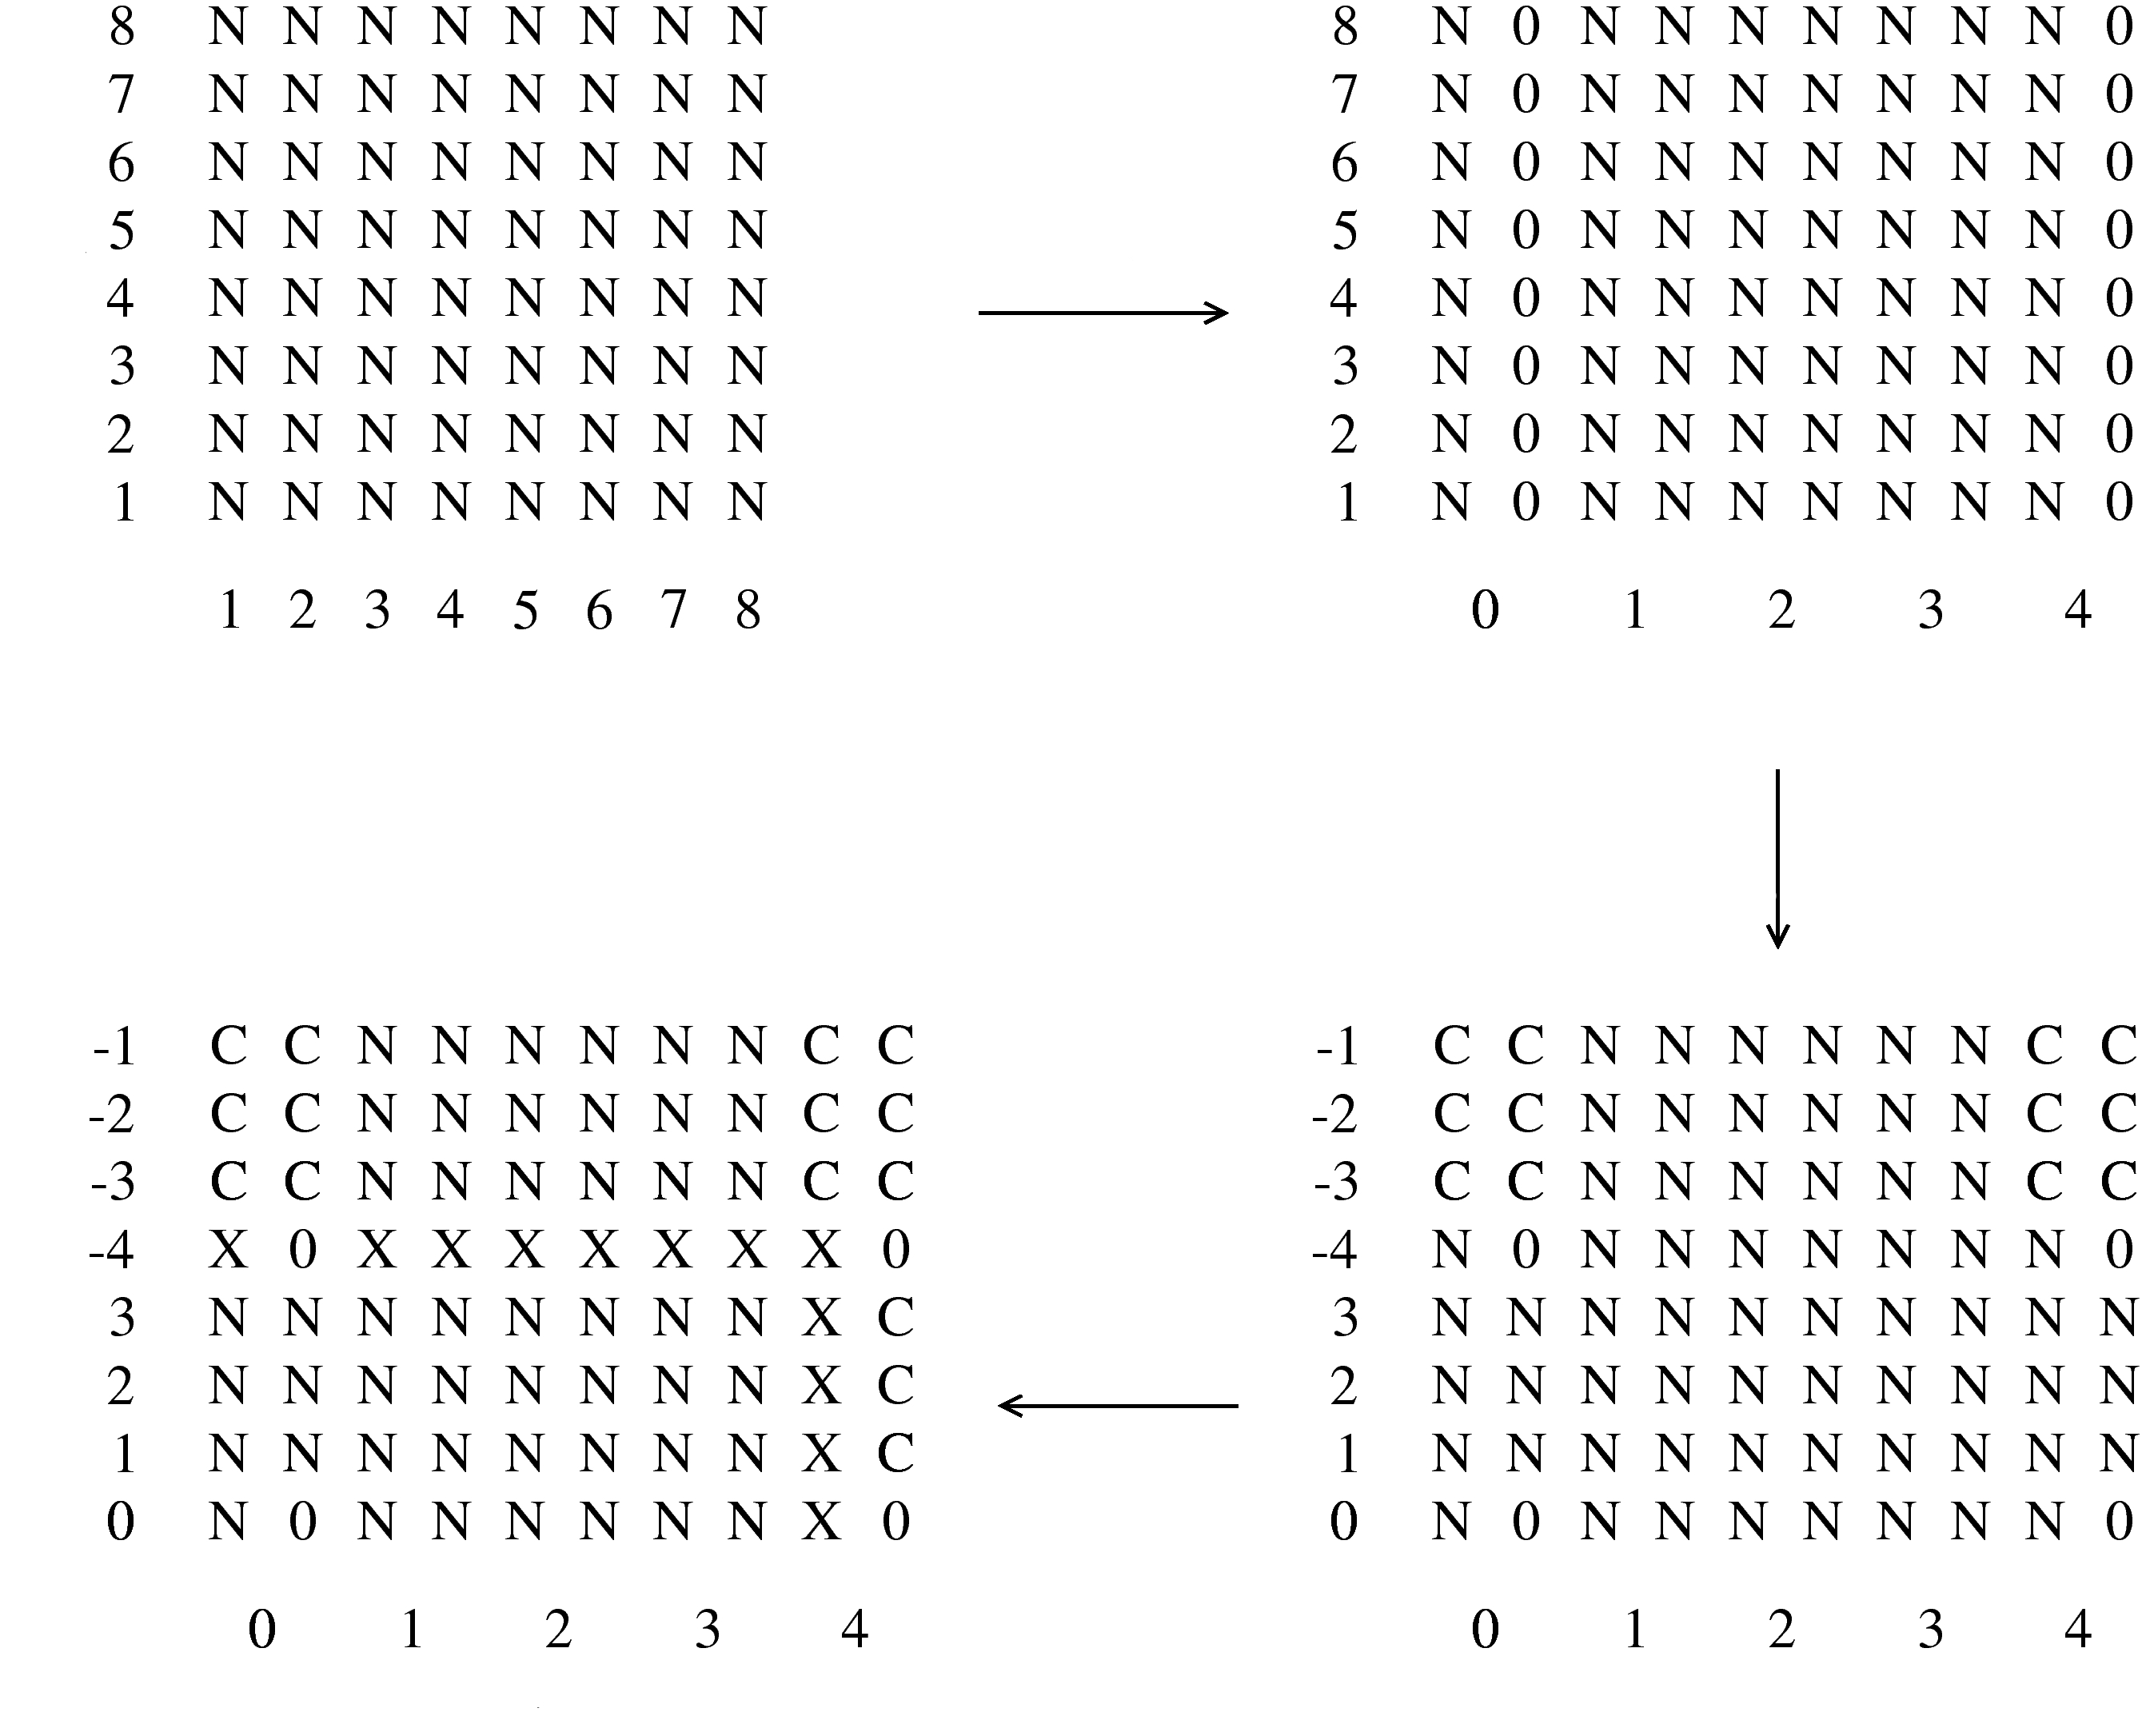
\includegraphics[width=0.80\textwidth]{oddball}
\put(-51,65){$\text{FFT}_x$}
\put(-15,38){$\text{FFT}_z$}
% Upper left
\put(-75,46){$x$}
\put(-95,65){$z$}
% Upper right
\put(-17,46){$\alpha$}
\put(-40,65){$z$}
% Lower right
\put(-17,0){$\alpha$}
\put(-41,19){$\beta$}
% Lower left
\put(-72,0){$\alpha$}
\put(-96,19){$\beta$}
\put(-53,16){odd-balls}
\caption{Schematic figure of the 2D transformation from physical to
Fourier space and the oddball. A domain with $N=8$ in two dimensions
is first transformed from physical space with a total of $64$ numbers
on a $N\times N=8\times 8=64$ grid (\texttt{N} indicates an arbitrary
number) in the $x$- and $z$-directions. In spectral space, the
information is conserved, \emph{i.e.}\ 64 independent numbers on a
$N\times(N+2)=8\times 10=80$ grid (\texttt{C} indicates redundant data
due to complex conjugate and $0$ means zero). To make sure that the
resulting field in spectral space also corresponds to a realizable
field, the oddball wavenumbers have to be set to zero (marked with
\texttt{X}). Thus, we are left with $49$ independent numbers.}
\label{fig:oddball}
\end{figure}


% ====================================================================
\section{Parallelization}
% ====================================================================
The code supports both parallelization based on shared memory using
OpenMP and distributed memory using MPI. Both variants give good
speed-up on a variety of computers. For machines supporting
both MPI and OpenMP it is recommended to compare both
parallelizations, however, OpenMP is expected to be slightly more
efficient.

The parallelization (both OpenMP and MPI) is designed in such a way
that exactly the same operations in the same order are performed on
the data. This implies that -- provided that the compiler generates
similar code -- results of a serial run are binary the same as the
ones obtained from a parallel calculation. This applies in particular
to the velocity and pressure fields, statistics files, two-point
correlations and saved planes.


% --------------------------------------------------------------------
\subsection{OpenMP} 
% --------------------------------------------------------------------
The OpenMP parallelization is implemented in a straight-forward way
around the loops calling \esub{nonlinbl}, \esub{linearbl},
\esub{nonlinp} and \esub{linearp}. Additionally, one loop in
\esub{ffun} and the computation of statistics in \esub{boxxys} is also
parallelized.  These parallel parts are the ones corresponding to the
majority of the work performed during time integration. Note that most
of the two-dimensional working arrays have an additional dimension
corresponding to the number of threads used. Thereby it is assured
that these work arrays are thread-private. Moreover, the first
threaded use of these work arrays is done by the correct thread, such
that for certain processor architectures independent memory busses are
assigned.

There is no strict upper limit on the number of OpenMP threads.
However, the number of planes in both the wall-normal direction and
spanwise direction is given by \epar{nyp} and \epar{nz},
respectively. Therefore these numbers can be considered natural upper
limits for the number of threads that could still lead to a
performance increase.


% --------------------------------------------------------------------
\subsection{MPI} 
% --------------------------------------------------------------------
In the present MPI parallelization, the main storage
\epar{ur}, \epar{ui} of the code is distributed among the processors
along the spanwise $z$ direction. Communication is therefore necessary
to evaluate the nonlinear terms in physical space. Hence, at the
beginning of the subroutines \esub{nonlinbl} and \esub{nonlinp}, a
global data transpose has to be performed. This is accomplished by
accessing the main storage via the functions \esub{getpxz} and
\esub{putpxz}, which internally take care of collecting the relevant
data of a $xz$-plane from all processors. Note that \esub{getpxz} and
\esub{putpxz} need to be called from all processors at the same time,
and that these functions always operate on \epar{nproc} consecutive
wall-parallel planes.

The global communication in \esub{getpxz} and \esub{putpxz} is
implemented in two different ways. On the one hand, the standard
\texttt{MPI\_ALLTOALL} library function can be used. However, to fit
with the data structure of the code, user-defined data types involving
\texttt{MPI\_TYPE\_STRUCT} and \texttt{MPI\_UB} have to be used. On
the other hand, a hand-written alternate version is also included,
which is based on explicit point-to-point send and receive
statements. Both version of \esub{getpxz} and \esub{putpxz}
essentially perform similarly and exhibit approximately the same
memory requirement. The hand-written version is chosen as the standard
for the present release. Further details on the implementation of the
MPI communication can be found in \cite{Alvelius-Skote}. Note that
this reference is based on an older version of the code, not
supporting all the features of the new code release.

The main storage is distributed among the processors. Therefore, the
memory footprint is also reduced by employing multiple MPI
processes. However, since each process needs to have a certain amount
of two- and one-dimensional work arrays, the decrease in memory
requirement is not linear. Note that all the large permanent storage
is allocated/declared in the main Fortran function \esub{bla}, which
allows a simple estimate on the memory required by each process.

The distribution of the data along the spanwise direction imposes the
natural upper limit of the possible processors to be
\epar{nz}. Moreover, \epar{nz} needs to be evenly divisible by the
number of processors, \epar{nproc}. The code has been shown to scale
essentially linearly up to \epar{nz$/$2} processors on various
distributed-memory architectures.


% ####################################################################
\chapter{File formats}
% ####################################################################
This section contains the formats of the most important input and output
files that are used by the \esoft{Simson} programs.

% ====================================================================
\section{Compile time parameter file \efilehead{par.f}}\label{sec:parfile}
% ====================================================================
The parameter file \efile{par.f} needs to be adjusted to fit the
numerical experiment at hand before starting to compile
\esoft{Simson}. Below follows a short description of these parameters.

The number of spectral modes in each direction is set by the
parameters \epar{nx}, \epar{ny} and \epar{nz}.  The following
restrictions apply: \epar{nx} and \epar{ny$-$1} must be even and
factorable by 2, 3 and 5, \epar{nz} must be factorable by 2, 3, 5 and
at least 2. Note that \epar{ny} is the number of Chebyshev polynomials
and thus is equal to $N_y+1$ used in chapter~\ref{sec:theory}.
 
Dealiasing, \emph{i.e.}\ padding to remove aliasing errors, can be
switched on (1) or off (0) independently for each direction by the
flags \epar{nfxd}, \epar{nfyd} and \epar{nfzd}.  If dealiasing in the
respective direction is used \epar{nx}, \epar{ny$-$1} must be
divisible by 4, and \epar{nz} must be divisible by 2.

There is an option to run 2 1/2 dimensional simulations, \emph{i.e.},
simulations of flow in a two dimensional geometry with all three
velocity components non-zero, which is sometimes called the infinite
swept flow (two dimensional flow is a special case of this). In this
case the spanwise parameters should be set to \epar{nz} $=1$,
\epar{nfzd} $=0$ and the limitations on \epar{nz} given above do not
apply. % \epar{nfzsym} $=0$ also

The parameter \epar{nthread} determines the maximum number of OpenMP
threads the code should be compiled for. The parameter \epar{nproc}
specifies the number of processors that should be used for the MPI
parallelization. Note that it is possible to combine OpenMP and MPI
parallelization (experimental).

To collect run-time statistical data during a simulation, several
parameters are used to define the storage requirements of these data
sets. The maximum number of two-dimensional $x-y$ velocity statistics
collected is given by \epar{nxys} (at the moment, 96 statistics are
implemented, see section \ref{sec:xysfile}. The number of statistics
involving the scalars is given by \epar{nxysth} (maximum 35). Note
that these statistics are taken for each scalar separately. The
parameter \epar{mcorr} sets the maximum number of spanwise two-point
correlations. The maximum number of time series is given by
\epar{mser}. The parameter \epar{msamp} is the size of the array
storing the time-series during run-time between writing them out to
disk and it is therefore required to be at least \epar{ixyss$/$ixys}
(see section \ref{sec:blafile}).

To allow for simultaneous calculation of velocities and pressure, the
parameter \epar{pressure} should be set to 1. The temperature can also
be computed as a passive scalar field by setting \epar{scalar} to 1 or
higher. By setting \epar{scalar} larger than one, multiple passive
scalar fields with individual Prandtl numbers and scalar boundary
conditions can be computed simultaneously.

%To achieve maximum performance the parameters \epar{mby} and
%\epar{mbz} can be changed from the default value 1, see
%section~\ref{sec:exe}. Note that \epar{nz} must be divisible by
%\epar{mbz}.

%The $z$-symmetry can be used to reduce computation time and storage by
%setting \epar{nfzsym} $=1$. If this is done \epar{nz} must be divisible
%by 4, and if used simultaneously with dealiasing in the $z$-direction
%\epar{nz} must be divisible by 8.

All other parameters in the \efile{par.f} file are computed and should
not be changed manually.  Note that most subroutines must be
recompiled after changing \efile{par.f}. An example of the user
relevant part of a \efile{par.f} file is given in table
\ref{tab:par-file}.
\begin{table}
\begin{verbatim}
.
.
c
c     Number of spectral modes
c
      parameter (nx=128,ny=121,nz=128)
c
c     Number of processors (MPI)
c
      parameter (nproc=1)
c
c     Number of threads (OpenMP)
c
      parameter (nthread=1)
c
c     Statistics
c
      parameter (nxys  =  96)
      parameter (nxysth=  35)
      parameter (mcorr =  30)
      parameter (mser  =  20)
      parameter (msamp =  16)
c
c     Pressure (0/1)
c
      parameter (pressure=1)
c
c     Passive scalars
c
      parameter (scalar=0)
c
c     Dealiasing flags
c
      parameter (nfxd=1,nfyd=0,nfzd=1)
c
c     Number of waves for freestream OS-eigenmodes
c
      parameter (osnf=250)
c
c     Number of points in base flow
c
      parameter (mbla=20001)
.
.
\end{verbatim}
\caption{An example of the user specific part of the compile time
parameter file \efile{par.f}.}
\label{tab:par-file}
\end{table}


% ====================================================================
\section{Runtime parameter file \efilehead{fsc.i}}\label{sec:fscfile}
% ====================================================================
The file \efile{fsc.i} is formatted and sequential.  Comments can be
put after data on lines not containing character input. This file is
read when running \esoft{fsc} in order to create a similarity solution
for boundary layer flows.
\begin{enumerate}
\item \epar{m} Power law exponent; \textit{real}.
\item \epar{n} Wall-normal resolution; \textit{integer}.
\item \epar{eps} Convergence criterion; \textit{real}.
\item \epar{ymax} Box height; \textit{real}.
\item \epar{scalar} The number of scalars. If non-zero, items a) and
b) are repeated for each passive scalar; \textit{integer}.
\begin{enumerate}
\item \epar{pr} Prandtl number; \textit{real}.
\item \epar{m1} Scalar exponent; \textit{real}. Note that
\epar{m1} $=0$ corresponds to an isothermal boundary condition, whereas
\epar{m1} $=0.5$ can be used for a iso-flux boundary condition.
\end{enumerate}
\end{enumerate}


% ====================================================================
\section{Runtime parameter file \efilehead{bls.i}}\label{sec:blsfile}
% ====================================================================
The file \efile{bls.i} is formatted and sequential. Comments can be
put after the data on lines not containing character input. For
boundary layer flows all input is non-dimensionalized with the
displacement thickness and the free-stream velocity at $x=0$ and
$t=0$. This file is read when running \esoft{bls} to generate initial
velocity fields, see also section~\ref{sec:geninit}. Contents line by
line:
\begin{enumerate}
\item \epar{namnin} Optional input velocity field file name;
\textit{character*80}.\\
The base flow can be given in the form of an
input velocity field file.
\item \epar{namnut} Output velocity file name; \textit{character*80}.
\item \epar{re} The Reynolds number;
\textit{real}.
\item \epar{xlb} The length of the computational box; \textit{real}.\\
The streamwise extent of the box must for spatially developing flows
include the length of the fringe region, which is typically set to
30--100 displacement thicknesses.
\item \epar{h2} The height of the computational box; \textit{real}.\\
In case of boundary layer flow the vertical extent of the box must
include the whole boundary layer. Depending on the choice of
free-stream boundary condition, the box may include only the boundary
layer or a few times more.  The sufficiency of the box height may be
investigated through numerical experiments.
\item \epar{zlb} The width of the computational box; \textit{real}.
\item \epar{fltype} Base flow type; \textit{integer}.\\
See table \ref{tab:flowtypes} on page \pageref{tab:flowtypes} for a
complete list of flow types.
\begin{enumerate}
\item If \epar{fltype} $= -1$ or $\ge$ 7: \epar{rlam} The acceleration
exponent of the velocity in the free-stream; \textit{real}.
\item If \epar{fltype} $= -2$ or $\ge$ 8: \epar{spanv} The spanwise
free-stream velocity; \textit{real}.
\item If \epar{fltype} $\ge$ 4: \epar{bstart} The streamwise position
of the start of the blending of the base flow; \textit{real}.
\item If \epar{fltype} $\ge$ 4: \epar{blength} The length of base flow
blending region; \textit{real}.
\end{enumerate}
The base flow can either be parallel or spatially developing. The
parallel base flows currently span Poiseuille, Couette, Blasius,
Falkner--Skan and FSC corresponding to \epar{fltype} $=1$, 2, 3, $-1$
and $-2$ respectively. The spatially developing base flow can be
either Poiseuille (\epar{fltype} $=4$), Couette (\epar{fltype} $=5$),
Blasius (\epar{fltype} $=6$), Falkner--Skan (\epar{fltype} $=7$),
Falkner--Skan--Cooke (\epar{fltype} $=8$) or temporal flow with fringe
region (\epar{fltype} $=9$). For the three latter cases the
acceleration exponent \epar{rlam} for the streamwise free-stream
velocity must be given (\emph{i.e.}\ $m$ in $U=Cx^m$).  For
Falkner--Skan--Cooke (swept wedge) flow the spanwise velocity
\epar{spanv} in the free-stream must be specified. Note that the
spanwise direction is parallel to the leading edge of the wedge for
this case, and that the spanwise free-stream velocity is constant.
For spatially developing flows the base flow from the upstream and the
downstream end are blended in the fringe region. The start and
blending length must be specified. Typically the start is given as a
negative number \emph{i.e.}, the distance upstream of the inflow
boundary where the blend starts is given (see section
\ref{sec:spatfor}).
\item \epar{pert} Flag to generate flow field without base flow. Used
for simulations in perturbation mode; \textit{logical}.
\item \epar{ushift} The Galilei shift velocity. Set to 0 for no shift;
\textit{real}.
\item \epar{locdi} Flag to generate a localized disturbance;
\textit{logical}.
\begin{enumerate}
\item \epar{ditype} The type of disturbance, only useful values 1 to
4; \textit{integer}.
\item \epar{amp} The amplitude of a localized disturbance;
\textit{real}.
\item \epar{theta} The rotation angle \epar{theta} of the localized
disturbance in radians; \textit{real}.
\item \epar{xscale} The streamwise scale of the disturbance;
\textit{real}.
\item \epar{xloc0} Origin of the disturbance in $x$-direction;
\textit{real}.
\item \epar{yscale} The wall-normal scale of the disturbance;
\textit{real}.
\item \epar{zscale} The spanwise scale of the disturbance;
\textit{real}.
\item \epar{ipoly} The wall-normal distribution of the disturbance,
only useful values 1 to 4; \textit{integer}.
\end{enumerate}
The \epar{ditype} determines the type of disturbance. See
\efile{bls.i} for more information.

The localized disturbance example (\epar{ditype} $=1$) is governed by
the amplitude, the rotation angle, the length and spanwise scale. The
rotation angle is the angle by which the spanwise symmetric
disturbance is rotated about the $y$-axis.  The $x$-scale and the
$z$-scale of the disturbance are given to be applied to the
disturbance before rotation.  The form of the disturbance is given in
a coordinate system aligned with the disturbance:
\begin{equation}
\begin{aligned}
u'   & = 0\,, \\
v    & = {\partial \psi \over \partial z}\,, \\
w'   & = -{\partial \psi \over \partial y}\,, \\
\psi & =  -\text{amp} {x' \over x_{\text{sc}}} {z' \over z_{\text{sc}}} p\left({y \over y_{\text{sc}}}\right)
e^{-\left({x' \over x_{\text{sc}}}\right)^2-\left({z' \over z_{\text{sc}}}\right)^2}\,, \\
\end{aligned}
\end{equation}
where $p(s)$ is determined by \epar{ipoly}, see \efile{bls.i}. The
above can be written in terms of the vector potential as
$\mathbf{u}=\nabla\times(\psi,0,0)^T$. The no-slip boundary condition
is fulfilled due to $p(s)$, and periodicity is given provided that the
spanwise scale is small compared to the width of the domain.  The
relation between the disturbance aligned velocities and coordinates
(with $'$) and the computational box aligned ones is:
\begin{equation}
\begin{aligned}
x    & = x'  \cos(\theta) + z' \sin(\theta)\,, \\
z    & = -x' \sin(\theta) + z' \cos(\theta)\,, \\
u    & = w'  \sin(\theta)\,, \\
w    & = w'  \cos(\theta)\,.
\end{aligned}
\end{equation}
\item \epar{gaussian} Flag to generate a Gaussian shaped disturbance;
\textit{logical}.
\begin{enumerate}
\item \epar{amp} Disturbance amplitude; \textit{real}.
\item \epar{y0}  Wall-normal peak location; \textit{real}.
\item \epar{yscale1} Wall-normal scaling factor; \textit{real}.
\item \epar{walfa} Streamwise wavelength; \textit{real}.
\item \epar{wbeta} Spanwise wavelength; \textit{real}.
\end{enumerate}
\item \epar{waves} Flag to generate a pair of oblique waves;
\textit{logical}.
\begin{enumerate}
\item \epar{energy} Energy density of the waves; \textit{real}.
\item \epar{ystart} The lowest $y$-value of non-zero wave amplitude;
\textit{real}.
\item \epar{yend} The largest $y$-value of non-zero wave amplitude;
\textit{real}.
\item \epar{yrise} The switch distance from zero to max wave
amplitude; \textit{real}.
\item \epar{yfall} The highest $y$-value of non-zero wave amplitude;
\textit{real}.
\item \epar{walfa} Streamwise wave number of the waves; \textit{real}.
\item \epar{wbeta} Spanwise wave number of the waves; \textit{real}.
\end{enumerate}
\item \epar{os} Flag to use tabulated eigenmodes; \textit{logical}.
\item \epar{specm} Spectral space mode; \textit{logical}.
\begin{enumerate}
\item \epar{amp} Amplitude; \textit{real}.
\item \epar{y0}  Wall-normal peak location; \textit{real}.
\item \epar{yscale1} Wall-normal scaling factor; \textit{real}.
\item \epar{nalfa} Streamwise wavenumber; \textit{real}.
\item \epar{nbeta} Spanwise wavenumber; \textit{real}.
\end{enumerate}
\item \epar{pertfromfile} Read perturbation from file;
\textit{logical}.
\begin{enumerate}
\item \epar{initcond\_u} File name of $u$-component;
\textit{character*80}.
\item \epar{initcond\_v} File name of $v$-component;
\textit{character*80}.
\item \epar{nalfa} Streamwise wavenumber; \textit{real}.
\item \epar{nbeta} Spanwise wavenumber; \textit{real}.
\end{enumerate}
\item \epar{noise} Flag to add noise; \textit{logical}.
\begin{enumerate}
\item \epar{ed} The mean energy density of the noise; \textit{real}.
\item \epar{nxn} The maximum streamwise wavenumber of the noise,
should be $\leq$ \epar{nx$/$2}; \textit{integer}.
\item \epar{nyn} The number of vertical Stokes modes in the noise,
should be even, $<$ \epar{ny}$\times$\epar{2$/$3}; \textit{integer}.
\item \epar{nzn} The maximum spanwise wavenumber of the noise, should
be odd, $<$ \epar{nz}; \textit{integer}.
\item \epar{seed} A random number seed in the range $-700000$ to $-1$;
\textit{integer}.
\end{enumerate}
The noise is in the form of Stokes modes, \emph{i.e.}, eigenmodes of
the flow operator without the convective term. They fulfill the
equation of continuity and the boundary condition of vanishing
velocity at the lower and upper boundaries. Although the actual
boundary condition may allow a non-zero amplitude at the free-stream
boundary the restriction of zero amplitude for the noise doesn't have
a large impact in practice.\\ If noise is used the mean energy density
must be given along with the number of wave numbers to be randomized
for each direction.  In the wall-normal direction the number of Stokes
modes to be randomized is given.  The same noise will be generated for
the same setting of this seed, if the physical size of the simulation
box is unchanged. In particular the resolution can be changed without
affecting the noise, as long as the number of grid points is
sufficient to resolve the noise modes. This is useful for convergence
studies.
\end{enumerate}


% ====================================================================
\section{Runtime parameter file \efilehead{bla.i}}\label{sec:blafile}
% ====================================================================
The file \efile{bla.i} is formatted and sequential. Comments can be
put after data on lines not containing character input or on separate
lines if the line begins with \texttt{\#}. Contents line by line:
\begin{enumerate}
\item \epar{date} Version of the \efile{bla.i} file. The version has
to match the version of \esoft{bla}. The format of the version is
YYYYMMDD; The current version is dated 20070716. \textit{integer}.
\item \epar{namnin} Input velocity file name; \textit{character*80}.
\item \epar{namnut} Output velocity file name; \textit{character*80}.
\item \epar{tmax} The final simulation time; \textit{real}.
\item \epar{maxit} The maximum number of iterations to simulate;
\textit{integer}.
\item \epar{cpumax} The maximum CPU time in seconds; \textit{real}.
\item \epar{wallmax} The maximum wall clock time in seconds;
\textit{real}.\\
The input and output file names and the final time \epar{tmax}
determine the scope of the simulation, in addition setting the maximum
number of iterations puts a limit on the number of iterations to be
taken through the main time step loop.  The latter parameter is useful
with variable time stepping in a batch environment to ensure that the
execution terminates before running out of execution time. If the
maximum number of iterations is used before the final time is reached
the execution will terminate normally by saving the present velocity
field to the output velocity file. Note that the physical time step
consists of three or four iterations.  The execution will only stop
after completing an integer number of physical time steps. If adaptive
time stepping is used the program will adjust the final four time
steps so that it reaches exactly the final time. You can also control
maximum execution time by giving either the maximum CPU time
(\epar{cpumax}) or maximum wall clock time (\epar{wallmax}) for batch
jobs. If one of the stop criteria is not to be used, specify a
negative number.
\item \epar{write\_inter} Write intermediate velocity field whenever
statistics are written to disk (\emph{i.e.}\ every \epar{ixyss} steps,
see below); \textit{logical}.
\item \epar{dt} The time step length; \textit{real}.\\
\epar{dt} is the length of the time step, if it is set $\le 0$ the
adaptive time stepping is used. The time step is regulated to keep the
CFL number close to \epar{cflmax}, which is set by the next parameter.
\item \epar{nst} The number of stages in the time discretization;
\textit{integer}.\\
The parameter \epar{nst} selects between the different formulas for
the explicit time discretization (3 three stage Runge--Kutta, 4 four
stage Runge--Kutta). The 4 stage Runge--Kutta method is about 20\%
more efficient than the 3 stage version.
\item \epar{cflmaxin} The maximum CFL number; \textit{real}.\\
The maximum convective stability limit is $\sqrt{3}$ for the three
stage Runge--Kutta and $\sqrt{8}$ for the four stage Runge--Kutta.
When using a fringe region the time step is also limited by the
numerical stability for the damping term, this is $1.75/$\epar{fmax}
for the three stage RK and $1.96/$\epar{fmax} for the four stage RK
(\epar{fmax} is the max strength of the fringe region, see below). If
\epar{dt} is set $<0$ then $-\epar{dt}$ is used as an additional limit
on the variable time step. The parameter \epar{cflmaxin} is a factor
indicating with fraction of the maximum stability limit should be used
for dynamic time-stepping. A value of about 0.8 is recommended.
\item \epar{xl} The new box length. If lower than the length read from
the velocity field, the velocity field length will be used;
\textit{real}.
\item \epar{varsiz} Flag to allow read of a velocity field of
different size than the code is compiled for; \textit{logical}.\\
If \epar{varsiz} is set true the program may start from an input field
of a different resolution than the program is compiled for.  The
spectral coefficients are padded with zeroes or truncated to achieve a
spectrally accurate interpolation.  However, the resolution cannot be
reduced in the normal direction as the truncated field in general will
not fulfill the equation of continuity and the boundary conditions.
\item \epar{rot} The angular velocity of the coordinate frame around
the $z$-axis. For non-rotating flows it should be set to zero;
\textit{real}.
\item \epar{cflux} Constant mass flux; \textit{logical}. Only
effective for channel flow (\epar{fltype $=1$}). If \epar{cflux} is
false:
\begin{enumerate}
\item \epar{retau} Target Reynolds number $\mathit{Re}_{\tau}$;
\textit{real}.  The pressure gradient is specified such that the
required skin friction is obtained.
\end{enumerate}
\item \epar{pert} Perturbation equations; \textit{logical}. Solve the
Navier--Stokes equations in perturbation form (\ref{eq:nsdist}). The
base flow should be a converged solution to the Navier--Stokes
equations, \emph{i.e.}\ preferably a steady simulation result. If
\epar{pert} is true:
\begin{enumerate}
\item \epar{lin} Linear simulation; \textit{logical}.
\end{enumerate}
\item \epar{ibc} The free-stream boundary condition number;
\textit{integer}.\\
A number of these boundary conditions makes the numerical scheme
unstable. Among the stable boundary conditions, the most used for
boundary-layer cases are number 101 and 110. A complete list of
available conditions are given in table
\ref{tab:boundary-condition-list} on page
\pageref{tab:boundary-condition-list}. See also section~\ref{freebc}
for more information about the different boundary conditions. Note
that for channel flow and Couette flow \epar{ibc} $=0$ should be
chosen.
\item Boundary conditions for passive scalars. The following
parameters are read \epar{scalar} times.
\begin{enumerate}
\item \epar{tbc} The boundary condition number (from 0 to 3);
\textit{integer}.
\item If \epar{tbc} $=0$
\begin{enumerate}
\item \epar{theta0\_low} Value of scalar at lower boundary;
\textit{real}.
\item \epar{theta0\_upp} Value of scalar at upper boundary;
\textit{real}.
\end{enumerate}
\item If \epar{tbc} $=1$
\begin{enumerate}
\item \epar{dtheta0\_low} Derivative of scalar at lower boundary;
\textit{real}.
\item \epar{theta0\_upp} Value of scalar at upper boundary;
\textit{real}.
\end{enumerate}
\item If \epar{tbc} $=2$
\begin{enumerate}
\item \epar{theta0\_low} Value of scalar at lower boundary;
\textit{real}.
\item \epar{dtheta0\_upp} Derivative of scalar at upper boundary;
\textit{real}.
\end{enumerate}
\item If \epar{tbc} $=3$
\begin{enumerate}
\item \epar{dtheta0\_low} Derivative of scalar at lower boundary;
\textit{real}.
\item \epar{dtheta0\_upp} Derivative of scalar at upper boundary;
\textit{real}.
\item \epar{theta0\_upp} Value of scalar at upper boundary;
\textit{real}.
\end{enumerate}
\end{enumerate}
\item \epar{cim} Flag to use Chebyshev integration method. If false
the tau method is used; \textit{logical}. If \epar{cim} is true:
\begin{enumerate}
\item \epar{icorr} Flag to use integration correction;
\textit{logical}.\\
The combination of using integration correction and boundary
conditions other than of Dirichlet type may lead to numerical
instability. The flag is normally set false.
\end{enumerate}
\item \epar{gall} Flag to compute and use a Galilei transformation 
in both streamwise and spanwise direction to increase the maximum
stable time step; \textit{logical}.\\
Presently only supported for temporal flows. The output (velocity
fields, statistics) are corrected for the shifted walls, \emph{i.e.}\
the shift velocity is added to the velocity components, and the flow
field is periodically shifted by the appropriate value.
\item \epar{suction} Flag to use constant suction at lower wall;
\textit{logical}. If \epar{suction} is true:
\begin{enumerate}
\item \epar{asbl} Asymptotic suction boundary layer;
\textit{logical}. If \epar{asbl} is false:
\begin{enumerate}
\item \epar{vsuc} Suction rate; \textit{real}.
\end{enumerate}
\end{enumerate}
\item \epar{spat} Flag to perform spatial simulation; \textit{logical}.\\
If \epar{spat} is false \esoft{bla} program performs a temporal
simulation. For spatial simulations a number of parameters specifying
the fringe region must be given, see section~\ref{sec:spatfor}. Items
a) through l) are read only if \epar{spat} is true.
\begin{enumerate}
\item \epar{tabfre} Tabulated free-stream velocity; \textit{logical}.\\
To use a tabulated free-stream velocity the flag \epar{tabfre} is set
true.  The format of the free-stream velocity file is given in
section~\ref{sec:frefile}. If \epar{tabfre} is true:
\begin{enumerate}
\item \epar{namfre} Name of file containing
free-stream velocity table; \textit{character*80}.
\end{enumerate}
\item \epar{rbfl} Flag to use a 3D flow field
as a base flow; \textit{logical}.\\
To use a 3D flow file to define the base flow the flag \epar{rbfl} is
set true.  The format of the 3D flow file is given in
section~\ref{sec:velfile}. If \epar{rbfl} is true:
\begin{enumerate}
\item  \epar{nambfl} Name of file containing a
3D base flow; \textit{character*80}.
\end{enumerate}
\item \epar{fmax} Maximum strength of the fringe region;
\textit{real}.
\item \epar{fstart} $x$-position of the start of the fringe region;
\textit{real}.
\item \epar{fend} $x$-position of the end of the fringe region;
\textit{real}.
\item \epar{frise} The distance from the start of the fringe region to
the first point of maximum damping; \textit{real}.
\item \epar{ffall} The distance from the last point of maximum damping
to the end of the fringe region; \textit{real}.
\item \epar{ampob} The amplitude of oblique
waves forced in the fringe; \textit{real}.\\
A pair of oblique waves can be generated in the fringe region by
setting \epar{ampob} non-zero. The format of the waveform file
\efile{wave.dat} is given in section~\ref{sec:fwfile}.
\item \epar{amp2d} The amplitude of two dimensional
Tollmien--Schlichting wave forced in the fringe; \textit{real}.
\item \epar{osmod} Flag to use free-stream
turbulence modes; \textit{logical}. If \epar{osmod} is true:
\begin{enumerate}
\item \epar{osdamp}; \textit{logical}. Whether or not to account for
the spatial growth of the amplitudes in the fringe region.
\item \epar{osamp} The amplitude of free-stream turbulence modes
forced in the fringe; \textit{real}.
\item \epar{osfil} The name of the file containing the free-stream
turbulence modes; \textit{real}.
\end{enumerate}
\item \epar{streak} Generate streaks (one or two) in the
fringe;\textit{logical}. If \epar{streak} is true:
\begin{enumerate}
\item \epar{str\_nam1} Input file; \textit{character*80}.
\item \epar{ampst(1)} Amplitude; \textit{real}.
\item \epar{tsmoo(1)} Length of smooth turn on; \textit{real}.
\item \epar{tsmoo(2)} Length of smooth turn off; \textit{real}.
\item \epar{tsmst(1)} Start of smooth turn on; \textit{real}.
\item \epar{tsmend(1)} Start of smooth turn off; \textit{real}.
\item \epar{iampst} Initial amplitude of streak; \textit{real}.
\item \epar{str\_nam2} Input file; \textit{character*80}.
\item \epar{ampst(2)} Amplitude; \textit{real}.
\item \epar{tsmoo(3)} Length of smooth turn on; \textit{real}.
\item \epar{tsmoo(4)} Length of smooth turn off; \textit{real}.
\item \epar{tsmst(2)} Start of smooth turn on; \textit{real}.
\item \epar{tsmend(2)} Start of smooth turn off; \textit{real}.
\item \epar{phist} Relative phase($/\pi$) of streaks; \textit{real}.
\end{enumerate}
\item \epar{waves} Generate waves in the fringe; \textit{logical}. If
\epar{waves} is true:
\begin{enumerate}
\item \epar{waamp} Amplitude; \textit{real}.
\item \epar{wamoo} Smoothing; \textit{real}.
\item \epar{wamst} Start time; \textit{real}.
\item \epar{waiamp} Initial amplitude; \textit{real}.
\end{enumerate}
\end{enumerate}
If \epar{spat} is false: 
\begin{enumerate}
\item \epar{cdev} The reference speed for the
parallel boundary layer growth; \textit{real}. For temporal
simulations \epar{cdev} must be set to the reference speed of the
boundary layer growth, see section~\ref{sec:tempfor_bou}.
\end{enumerate}
\item \epar{sgs} To read the file \epar{sgs.i}, used to enable LES
mode; \textit{logical}.
\item \epar{isfd} To use selective frequency damping (0=off, 1=on);
\textit{integer}. If \epar{isfd} is 1:
\begin{enumerate}
\item \epar{sfdzero} Start from zero filtered field;
\textit{logical}. If false:
\begin{enumerate}
\item \epar{namnut\_sfd} Initial filtered field; \textit{character*80}.
\end{enumerate}
\item \epar{sfd\_delta} Temporal filter width; \textit{real}.
\item \epar{sfd\_chi} Temporal relaxation parameter; \textit{real}.
\end{enumerate}
\item \epar{imhd} To enable a magnetic field (MHD) (0=off, 1=on);
\textit{integer}. If \epar{imhd} is 1:
\begin{enumerate}
\item \epar{b0(1)} Component of the magnetic field in $x$-direction;
\textit{real}.
\item \epar{b0(2)} Component of the magnetic field in $y$-direction;
\textit{real}.
\item \epar{b0(3)} Component of the magnetic field in $z$-direction;
\textit{real}.
\item \epar{mhd\_n} Strength of the magnetic field. The direction of
the magnetic field \epar{b0(1)}, \epar{b0(2)}, \epar{b0(3)} will be
normalized to unity; \textit{real}.
\end{enumerate}
\item \epar{loctyp} to generate a localized volume force disturbance;
\textit{integer}.\\
The parameter \epar{loctyp} can take values from 1 to 8. Various
disturbances can be created. See \efile{locf.f} for more information.
The different values of \epar{loctyp} each requires a distinct number
of parameters in the file \efile{bla.i}, see \efile{rparambl.f} for
more information.  As an example, a localized volume force disturbance
to generate wave packets is created by setting \epar{loctyp} to 1.
\begin{enumerate}
\item \epar{ampx} Max amplitude of the localized
volume force disturbance in $x$-direction; \textit{real}.
\item \epar{ampy} Max amplitude of the localized
volume force disturbance in $y$-direction; \textit{real}.
\item \epar{ampz} Max amplitude of the localized
volume force disturbance in $z$-direction; \textit{real}.
\item \epar{xscale} Length scale of the
localized volume force disturbance in $x$-direction; \textit{real}.
\item \epar{xloc0} Origin of the localized
volume force disturbance in $x$-direction; \textit{real}.
\item \epar{yscale} Length scale of the
localized volume force disturbance in $y$-direction; \textit{real}.
\item \epar{zscale} Length scale of the
localized volume force disturbance in $z$-direction; \textit{real}.
\item If \epar{zscale} $<0$: \epar{lskew} The
obliqueness of waves of the localized volume force disturbance;
\textit{real}.
\item \epar{tscale} Time scale of the
localized volume force disturbance; \textit{real}.\\
If \epar{loctyp} is 1, the form of the localized disturbance is:
\begin{equation}
{ \left[ \begin{array}{c} F_1 \\ F_2 \\ F_3 \end{array} \right] } = 
{ \left[ \begin{array}{c} \text{amp}_x \\ \text{amp}_y \\ \text{amp}_z \end{array} \right] }
e^{-(y/y_{\text{sc}})^2} g(x,z) f(t)\,,
\end{equation}
where
\begin{equation}
\begin{aligned}
z_{\text{sc}}>0 \quad
g(x,z)&=e^{-((x-x_{\text{loc0}})/x_{\text{sc}})^2-(z/z_{\text{sc}})^2}\,, \\
z_{\text{sc}}<0 \quad
g(x,z)&=\cos(2\pi(z-x_{\text{lskew}})/z_{\text{sc}})e^{-{((x-x_{\text{loc0}})/x_{\text{sc}})^2}}\,,
\end{aligned}
\end{equation}
and
\begin{equation}
\begin{aligned}
t_{\text{sc}}>0 \quad f(t)& = e^{-(t/t_{\text{sc}})^2}\,, \\
t_{\text{sc}}<0 \quad f(t)& = S(-t/t_{\text{sc}}))\,, \\
t_{\text{sc}}=0 \quad f(t)& = 1\,,
\end{aligned}
\end{equation}
and
\begin{equation}
\begin{aligned}
S(x)    & = \left\{ \begin{array}{ll}
 0\,,   & \quad x\le 0\,, \\
 1/(1+e^{(1/(x-1) + 1/x)})\,, & \quad 0 < x < 1\,, \\
 1\,,   & \quad x\ge 1\,.
\end{array}
\right.
\end{aligned}
\label{eq:s}
\end{equation}
\end{enumerate}
\item \epar{tripf} Flag to generate a random ``sand paper'' volume
force trip strip running in the spanwise direction;
\textit{logical}. If \epar{tripf} is true:
\begin{enumerate}
\item \epar{tamps} Maximum steady amplitude of the trip;
\textit{real}.
\item \epar{tampt} Maximum time varying amplitude of the trip;
\textit{real}.
\item \epar{txsc} Streamwise length scale of the trip; \textit{real}.
\item \epar{tx0} Streamwise origin of the trip; \textit{real}.
\item \epar{tysc} Wall-normal length scale of the trip; \textit{real}.
\item \epar{nzt} Number of Fourier modes in the spanwise direction of
the trip; \textit{integer}.
\item \epar{tdt} Time interval between change of the time dependent
part of the trip; \textit{real}.
\item \epar{seed} Negative number in the range $-700000$ to $-1$ to
initialize the random number generator for the trip; \textit{integer}.
\end{enumerate}
The trip force can be used to generate turbulence or noise at lower
amplitude levels to test the stability of a boundary layer or flow
structure. The trip has a steady amplitude \epar{tamps} and a time
dependent amplitude \epar{tampt} which allow both steady and time
varying trips to be generated. The volume force has one continuous
time derivative and is independent of the time discretization. The
random numbers are generated such that if the random number
\epar{seed} and other trip parameters are unchanged, the same trip
forces are generated. This is true even if the simulation is split
into two or more runs. For every run beyond the first the random
number generator is run forward to the correct state. The form of the
volume force, which is directed normal to the wall, is as follows:
\begin{equation}\label{eq:trip}
F_2=\exp(-\{(x-t_{x0})/t_{\text{xsc}}\}^2-(y/t_{\text{ysc}})^2) f(z,t)\,,
\end{equation}
where
\begin{equation}
f(z,t)=t_{\text{amps}} g(z) + t_{\text{ampt}} ((1-b(t))h^i(z)+b(t) h^{i+1}(z))\,,
\end{equation}
and
\begin{equation}
\begin{aligned}
i    & = \mbox{int}(t/t_{dt})\,, \\
b(t) & = 3p^2-2p^3\,, \\
p    & = t/t_{dt}-i\,.
\end{aligned}
\end{equation}
Here $g(z)$ and $h_{i}(z)$ are Fourier series of unit amplitude with
\epar{nzt} random coefficients. The trip forcing generates noise with
a uniform distribution over all frequencies lower than the cutoff
frequency corresponding to $2\pi/t_{dt}$.
\item \epar{wbci} Boundary conditions at wall; \textit{integer}.\\
\epar{wbci} can be set from $-2$ to 2. If \epar{wbci} is not equal to
zero, additional parameters must be provided. See \efile{rparambl.f},
\efile{rparamwallrough.f} and \efile{cwallbc.f}.  The example below is
for \epar{wbci} set to 1.
\begin{enumerate}
\item \epar{amp} Max amplitude of the localized blowing/suction;
\textit{real}.
\item \epar{damp} Damp amplitude. No effect if one;
\textit{real}.
\item \epar{xstart} Start position of disturbance; \textit{real}.
\item \epar{xend} End position of disturbance; \textit{real}.
\item \epar{xrise} Rise length of disturbance; \textit{real}.
\item \epar{xfall} Fall length of disturbance; \textit{real}.
\item \epar{zbet} Spanwise variation; \textit{real}.
\item \epar{tomeg} Time variation; \textit{real}.
\end{enumerate}
The form of this boundary condition is
\begin{equation}
v |_{y=0}=\text{amp}  f(x)  \cos(z_{\text{bet}} z) \sin(t_{\text{omeg}} t)\,,
\end{equation}
where
\begin{equation}
f(x)=S\left({{x-x_{\text{start}}}\over x_{\text{rise}}}\right)
    -S\left({{x-x_{\text{end}}}\over x_{\text{fall}}+1}\right),
\end{equation}
and $S(x)$ is given by equation (\ref{eq:s}). \\
If \epar{wbci} is set to $-1$ the wall-roughness model is turned on,
see section \ref{sec:roughness}. Then, an extra input file
containing the relevant parameters has to be supplied:
\begin{enumerate}
\item \epar{wallroughinput} Name of input file for wall roughness;
\textit{character*80}.
\end{enumerate}
Details about the required parameters for the roughness model can be
found in \efile{rparamwallrough.f} and in section
\ref{sec:wlroughfile}.\\
If \epar{wbci} is set to $-2$ a jet profile is imposed, see section
\ref{sec:jet-in-crossflow} for more details.
\item \epar{icfl} Number of time iterations between calculation of the
CFL number; \textit{integer}.\\
If the CFL number is computed each iteration this adds a few percent
to the execution time, but since it is used to regulate the time step
it should not be computed too sparsely, preferably every complete time
step, \emph{i.e.}\ \epar{icfl} = \epar{nst}.
\item \epar{iamp} Number of time iterations between calculation of rms
amplitudes; \textit{integer}. If \epar{iamp} $>0$ items a) and b) are
read.
\begin{enumerate}
\item \epar{namamp} Output file for rms amplitudes;
\textit{character*80}.
\item \epar{fileurms} Write $u$-rms velocities;
\textit{logical}.
\end{enumerate}
As for the CFL number continuous calculation of the amplitude costs a
number of percent in execution speed.  If \epar{iamp} $=0$ no
amplitudes will be calculated and no amplitude file will be
written. To get the correct time accuracy \epar{iamp} should be an
integer multiple of \epar{nst}.
\item \epar{longli} Flag to generate amplitude for each horizontal
plane ($y$-value). Applies both to rms amplitudes and wave component
amplitudes.\\
If \epar{longli} is set true the program will produce $y$-dependent
statistics and write these to the amplitude files, both for the global
statistics and statistics by wavenumber. The statistics files can
become quite large if the flag is set true.
\item \epar{iext} Number of time iterations between calculation of
extremum amplitudes; \textit{integer}.\\
To get the correct time accuracy \epar{iext} should be an integer
multiple of \epar{nst}. If \epar{iext} $=0$ no extremum amplitudes
will be calculated. If \epar{iext} $>0$ item a) is read.
\begin{enumerate}
\item \epar{namext} Output file for extremum
amplitudes; \textit{character*80}.
\end{enumerate}
\item \epar{ixys} Number of time iterations between calculation of 
$xy$-statistics; \textit{integer}.\\
The statistics can be analyzed with \esoft{pxyst}. The statistics
generated and the output file format are described in
section~\ref{sec:xysfile}. The file is written to every \epar{ixyss}
iterations, overwriting older data. To get the correct time accuracy
\epar{ixys} should be an integer multiple of \epar{nst}. If
\epar{ixys} $>0$ items a) through e) are read.
\begin{enumerate}
\item \epar{namxys} Output file for $xy$-statistics;
\textit{character*80}.
\item \epar{ixyss} Number of time iterations between saving of
$xy$-statistics data to file; \textit{integer}. If \epar{write\_inter}
is true, then also an intermediate velocity field is saved to the file
\efile{end.uu} (this name can be changed in \efile{rparambl.f}). A
crashed simulation can then be safely restarted from the saved
intermediate field without corrupting statistics taken during the run,
since the statistics and the velocity field are written out at the
same time instant.
\item \epar{txys} Time to start accumulation
of $xy$-statistics; \textit{real}.
\item \epar{corrf} Flag to save spanwise
two-point correlations; \textit{logical}.  The statistics generated
and the output file format are described in
section~\ref{sec:twopointfile}. If \epar{corrf} is true:
\begin{enumerate}
\item \epar{corrnam} Output file for two-point correlations;
\textit{character*80}.
\item \epar{ncorr} Number of positions to save two-point correlations;
\textit{integer}.\\
The list is then read from file \efile{two-point.dat}; the format of
this input file is a simple text file with at least \epar{ncorr} lines
specifying on each line the $x$ and $y$ coordinates and the quantity
to save. The possible quantities are the velocities, pressure, scalar
correlations and some selected correlations of derivatives (see file
\efile{boxxys.f} for details).
\end{enumerate}
\item \epar{serf} Flag to save time histories at given coordinates;
\textit{logical}. The statistics generated and the output file format
are described in section~\ref{sec:timeseriesfile}. If \epar{serf} is
true:
\begin{enumerate}
\item \epar{namser} Output file for time histories;
\textit{character*80}.
\item \epar{nser} Number of positions to save time histories;
\textit{integer}.\\
The list is then read from the input file \efile{probe.dat}; the
format of this input file is a simple text file with at least
\epar{nser} lines specifying on each line the $x$, $y$ and $z$
coordinates and an integer representing the quantity to save. The
possible quantities are the velocities, pressure, scalar, and the
various velocity and scalar derivatives (see file \efile{boxxys.f} for
details).
\end{enumerate}
\end{enumerate}
\item \epar{msave} The number of complete velocity fields to be saved
at specific times. If \epar{msave} $>0$, items a) and b) are repeated
for each file; \textit{integer}.
\begin{enumerate}
\item \epar{tsave} The time for which to save a field; \textit{real}.
%
\item \epar{nmsave} The name of the velocity file;
\textit{character*80}.
\end{enumerate}
\epar{msave} is the number of velocity fields to be saved, maximum
\epar{nsave} (set as a parameter in \efile{bla.f}). If larger than
zero the times and names of the files to be saved must be given.  If
the adaptive time stepping is used \esoft{bla} automatically adjusts
the time step to reach exactly the desired times.  For fixed time step
the save is done at the nearest time.
\item \epar{mwave} The number of wavenumber amplitudes to be saved. If
\epar{mwave} $>0$, item b) is repeated for each wavenumber;
\textit{integer}.
\begin{enumerate}
\item \epar{namwav} The name of the wave amplitude file;
\textit{character*80}.
\item \epar{kx} \epar{kz} The streamwise wavenumber as multiples of
the fundamental wavenumber $2\pi/x_L$, the spanwise wavenumber as
multiple of the fundamental wavenumber $2\pi/z_L$; both
\textit{integers}.
\end{enumerate}
\epar{mwave} sets the number of specific wavenumbers to calculate
amplitudes for.  For each wave, the $x$ and $z$ wavenumbers must be
specified as integers to be multiplied by $2\pi /x_L$ and $2\pi /z_L$
respectively.  The wavenumbers are counted in the physical way for
positive and negative \epar{kz} and \epar{kx} zero and up, not in the
way of the internal storage. The wave amplitudes are calculated for
each of the six velocities and vorticities at intervals set by the
\epar{iamp} value.
\item \epar{npl} The number of planes to be continuously saved during
the simulation.  If \epar{npl} $>0$, items b) through e) are repeated
for each plane; \textit{integer}.
\begin{enumerate}
\item \epar{ipl} The saving interval for planes in number of
iteration; \textit{integer}.
\item \epar{tpl(i,1)} The type of plane to be saved, 1 for $xy$ and 2
for $xz$; \textit{integer}.
\item \epar{tpl(i,2)} The variable to be saved, \emph{i.e.}\ 1 for
$u$, 2 for $v$, 3 for $w$; \textit{integer}.
\item \epar{cpl} The coordinate for which to save the plane;
\textit{real}.
\item \epar{nampl} The name of the file in which to save the planes;
\textit{character*80}.
\end{enumerate}
\epar{npl} is the number of 2D planes to be saved every \epar{ipl}
iterations during the simulation. To get the correct time accuracy
\epar{ipl} should be an integer multiple of \epar{nst}. These files
can be visualized with \esoft{rps}. The format is described in
section~\ref{sec:planefile} below. The MPI version does currently not
support $yz$-planes.
\end{enumerate}

\begin{table}
\begin{tabular}{rl}
\hline
\hline
\epar{ibc} & Free-stream boundary condition types\\ 
\hline
     0     & $u=v=w=0$ \\
     1     & $Du=Dv=Dw=0$ \\
     2     & $D^2u=D^2v=D^2w=0$ \\
     3     & $D^3u=D^3v=D^3w=0$ \\
    10     & $Du+ku=Dv+kv=Dw+kw=0$ \\
    11     & $D^2u+kDu=D^2v+kDv=D^2w+kDw=0$ \\
    12     & $D^3u+kD^2u=D^3v+kDv=D^3w+kD^2w=0$ \\
    20     & $Dv+kv=D^2v+kDv=\omega=0$ \\
   100     & $u=U$, $v=V$, $w=W$ \\
   101     & $Du=DU$, $Dv=DV$, $Dw=DW$ \\
   110     & $Du+ku=DU+kU$, $Dv+kv=DV+kV$, $Dw+kw=DW+kW$ \\
   120     & $Dv+kv=DV+kV$, $D^2v+kDv=D^2V+kDV$, $\omega=0$ \\
   130     & $u=U$, $Du=DU$, $w=W$ \\
   140     & $u=U$, $Dv=DV$, $w=W$ \\
%   150     & $u=U$, $Du-vx=0$, $Dw=0$ \\
   150     & $u=U$, $Du-v_x=0$, $Dw=0$ for $\beta=0$ $^1$,\\ 
           & $Du=DU$, $Dv=DV$, $Dw=DW$ for $\beta\ne0$ (see 101) \\
   160     & $Dv=DV$, $Du-v_x=0$, $w=W$ for $\beta=0$ \\
           & $Du+ku=0$, $Dv+kv=0$, $Dw+kw=0$ (see 110) \\
           & or similar to 101 if added in \esub{evalbc.f} ``*0''. \\
   170     & $u=U$, $Du-v_x=0$, $Dw=0$ \\
\hline
\hline
\end{tabular}
\caption{Free-stream boundary conditions. Here $u,v,w$ are the
solution velocities and $U,V,W$ are the base flow velocities. The
velocity derivative normal to the boundary is indicated by $D$ and $k$
denotes the modulus of the horizontal wavenumber
($k^2=\alpha^2+\beta^2$). \newline
$^1$ Note that for the mean component $\alpha=\beta=0$ not both $u$ and $\vartheta$ can be prescribed. Therefore, it can be chosen directly in the code (\esub{linearbl.f}) which of those quantities to set.
}
\label{tab:boundary-condition-list}
\end{table}


% ====================================================================
\section{Runtime LES parameter file \efilehead{sgs.i}}\label{sec:lesfile}
% ====================================================================
The file \efile{sgs.i} is formatted and sequential.  Comments can be
put after data on lines not containing character input. This file is
read when running LES. Contents line by line:
\begin{enumerate}
\item \epar{date} Date to show which version of the \efile{sgs.i} file
that is needed; the current version is dated 20060909;
\textit{integer}.
\item \epar{iles} Type of SGS model used; \textit{integer}.\\
If \epar{iles} $=0$: no SGS model is used, \emph{i.e.}\ a DNS is
performed.\\
If \epar{iles} $=1$: the ADM-RT model is
used:
\begin{enumerate}
\item \epar{cutoff\_inv} Inverse cutoff wavenumber of the primary
filter; \textit{real}.
\item \epar{iord} Order of the high-pass filter;
\textit{integer}.
\item \epar{chi} Model coefficient $\chi$,
$\chi=0$ activates the dynamic procedure; \textit{real}.
\end{enumerate}
If \epar{iles} $=2$: the standard Smagorinsky model is
used. 
\begin{enumerate}
\item \epar{cs} Model coefficient $C_S$, $C_S=0$ activates the dynamic
procedure; \textit{real}.
\item If \epar{cs} $=0$: \epar{ineg} Determines clipping behavior of
the dynamic procedure; \textit{integer}. \epar{ineg} $=0$, no
clipping, \epar{ineg} $=1$, clipping to positive $C_S$, \epar{ineg}
$=2$, clipping to positive total viscosity.
\end{enumerate}
If \epar{iles} $=3$: the high-pass filtered Smagorinsky model is
used. 
\begin{enumerate}
\item \epar{cutoff\_inv} Inverse cutoff wavenumber of the primary
filter; \textit{real}.
\item  \epar{iord} Order of the low-pass filter;
\textit{integer}.
\item  \epar{cs} Model coefficient $C_S$, $C_S=0$
activates the (consistent) dynamic procedure; \textit{real}.
\item If \epar{cs} $=0$: \epar{ineg} Determines clipping behavior of
the dynamic procedure; \textit{integer}. \epar{ineg} $=0$, no
clipping, \epar{ineg} $=1$, clipping to positive $C_S$, \epar{ineg}
$=2$, clipping to positive total viscosity.
\end{enumerate}
\end{enumerate}


% ====================================================================
\section{Velocity file}\label{sec:velfile} 
% ====================================================================
Format of a 3D velocity file. The format is used for any 3D input or
output from \esoft{bls}, \esoft{bla} and \esoft{cmp}. The file is
unformatted, sequential. This file can be visualized by \esoft{rit}.

\begin{description}
\item[Record 1:] Reynolds number; \textit{real}, Poiseuille (true) or
Couette flow (false); \textit{logical}, $x_L$; \textit{real}, $z_L$;
\textit{real}, the time for this field; \textit{real}, the length by
which the box has been shifted to the right since time zero;
\textit{real}, Prandtl number; \textit{real}, $m_1$ power law
exponent; \textit{real}. The last two parameters are repeated for each
scalar field.
\item[Record 2:] Number of spectral modes in the $x$-direction;
\textit{integer}, the number of points in the physical $y$-direction;
\textit{integer}, the number of spectral modes in the $z$-direction
reduced for symmetry; \textit{integer}, 0/1 no
$z$-symmetry/$z$-symmetry; \textit{integer}.
\item[Record 3:] Flow type \epar{fltype}; \textit{integer},
displacement thickness expressed in half box heights \epar{dstar};
\textit{real}.
\item[Record 4:] If \epar{fltype} $\ge 4$: start of blending region
\epar{bstart}, length of blending region \epar{blength}, if
\epar{fltype} $\ge 7$: acceleration exponent of streamwise free-stream
velocity \epar{rlam}, spanwise free-stream velocity \epar{spanv}. If
\epar{fltype} $= -1$: \epar{rlam} and if \epar{fltype} $= -2$
\epar{rlam} and \epar{spanv}. For other values of \epar{ fltype} this
record is omitted.
\item[Record 5:] The $u,v,w$-velocities in Fourier $x,z$ and physical
$y$ space.  One record contains \epar{nx$/$2} complex coefficients in
normal Fortran format. The records are stored in \texttt{y},
\texttt{z}, \texttt{i} order with \texttt{y} varying the fastest and
\texttt{i} the slowest.  The number of points in the $y$-direction is
\epar{nyp} and the number of points in the $z$-direction is
\epar{nzc}. Total number of records \epar{nyp$\times$nzc$\times$3}.
\item[Record 6 - \ldots] The $\theta_i$ scalar distribution in Fourier
$x$, $z$ and physical $y$ space (similar to the velocities). The number
of records depends on the number of scalars at compile time.
\end{description}


% ====================================================================
\section{Pressure file}\label{sec:prefile} 
% ====================================================================
Format of a 3D pressure file. The format is the same as for the
velocity file, except the last record which contains only the
pressure. This file can be visualized by \esoft{rit}.


% ====================================================================
\section{Amplitude file}\label{sec:ampfile}
% ====================================================================
Formatted, sequential. To be analyzed with the tools \esoft{pamp1} and
\esoft{pamp2}. The rms-levels are averages over the physical box. For
each time three records are saved:
\begin{description}
\item[1:] Time; \textit{real}, $u_{\text{rms}}$; \textit{real},
$v_{\text{rms}}$; \textit{real}, $w_{\text{rms}}$; \textit{real},
$\chi_{\text{rms}}$; \textit{real}, $\omega_{\text{rms}}$;
\textit{real}, $\vartheta_{\text{rms}}$; \textit{real},
$\omega^2/k^2$; \textit{real}, $DUuv$; \textit{real}, energy for
wavenumber zero; \textit{real}, $h^+$, \emph{i.e.}\ the box
half-height in wall units; \textit{real}.
\end{description}
If \epar{longli} is true then for each time the above is followed by
statistics by $y$-plane in descending $y$-coordinate order as follows:
\begin{description}
\item[2:] Mean squared streamwise velocity without Blasius base flow; \textit{real},
mean squared normal velocity; \textit{real},
mean squared spanwise velocity; \textit{real},
mean squared streamwise vorticity; \textit{real},
mean squared normal vorticity; \textit{real},
mean squared spanwise vorticity without Blasius base flow; \textit{real},
mean squared vorticity squared over wavenumber square average, no (0,0); \textit{real},
Reynolds stress average; \textit{real},
mean streamwise disturbance velocity squared; \textit{real},
mean spanwise disturbance velocity squared; \textit{real}.
\end{description}


% ====================================================================
\section{Wave amplitude file}\label{sec:wampfile}
% ====================================================================
Formatted, sequential. To be analyzed with the tools \esoft{pampw} and
\esoft{pampw2}. The data in this file is in internal scaling. For each
time the following data are saved:
\begin{description}
\item[1:] Time; \textit{real}, number of waves saved;
\textit{integer}, number of points in the $y$-direction;
\textit{integer}, Reynolds number; \textit{real}, fundamental
wavenumber in the $x$-direction; \textit{real}, fundamental wavenumber
in the $z$-direction; \textit{real}, flag \epar{longli}.
\item[2:] The wavenumber $\alpha$ as multiples of the fundamental
$2\pi/x_L$; \textit{integer}, the wavenumber $\beta$ as multiple of
the fundamental $2\pi/z_L$; \textit{integer}, $u_{\text{rms}}$;
\textit{real}, $v_{\text{rms}}$; \textit{real}, $w_{\text{rms}}$;
\textit{real}, $\omega_{\text{rms}}$; \textit{real}.\\
Item 2 is repeated for each wave.
\end{description}
If \epar{longli} is true then for each time the above is followed by
statistics by $y$-plane in descending $y$-coordinate order as follows:
\begin{description}
\item[3:] If the wavenumber is zero: $\hat{u}$ for each $y$-plane
(with the imaginary part zero), otherwise $\hat{v}$ for each
$y$-plane; \textit{complex}.
\item[4:] If the wavenumber is zero: $\hat{w}$ for each $y$-plane
(with the imaginary part zero), otherwise $\hat{\omega}$ for each
$y$-plane; \textit{complex}.
\end{description}
Items 3 and 4 are repeated for each wave.


% ====================================================================
\section{Extremum file}\label{sec:extfile}
% ====================================================================
Formatted, sequential. For each time the following data are saved:
\begin{description}
\item[1:] Time; \textit{real}.
\item[2:] Min $u-U_{\text{laminar}}$; \textit{real}, $x$-coordinate
for this minimum; \textit{real}.
\item[3:] $y$-coordinate; \textit{real}, $z$-coordinate; \textit{real}.
\item[4 - 5:] Same for  min $v$.
\item[6 - 7:] Same for  min $w$.
\item[8 - 9:] Same for  min $\chi$.
\item[10 - 11:] Same for  min $\omega$.
\item[12 - 13:] Same for  min $\vartheta$.
\item[14 - 15:] Same for  min $\vartheta-\vartheta_{\text{laminar}}$.
\item[16 - 29:] Same as 2 through 15 but for maximum.
\end{description}


% ====================================================================
\section{Plane velocity file}\label{sec:planefile}
% ====================================================================
Unformatted, sequential. This file can be visualized by \esoft{rps}.
\begin{description}
\item[Record 1:] Reynolds number; \textit{real}, \epar{.false.}  (this
is to be backward compatible with channel flow files);
\textit{logical}, $x_L$; \textit{real}, $z_L$; \textit{real}, the time
for this field; \textit{real}, the length by which the box has been
shifted to the right since time zero; \textit{real}.
\item[Record 2:] Number of spectral modes in the $x$-direction;
\textit{integer}, the number of points in the physical $y$-direction;
\textit{integer}, the number of spectral modes in the $z$-direction
reduced for symmetry; \textit{integer}, 0/1 no
$z$-symmetry/$z$-symmetry; \textit{integer}.
\item[Record 3:] The type of plane, 1 for $xy$-plane, 2 for
$xz$-plane; \textit{integer}, the variable number, \emph{i.e.}, 1 for
$u$, 2 for $v$, 3 for $w$; \textit{integer}, the coordinate of the
plane; \textit{real}, flow type \epar{fltype}; \textit{integer},
displacement thickness \epar{dstar} expressed in half box heights;
\textit{real}.
\item[Record 4:] Time; \textit{real}, the length by which the boxed
has been shifted to the right since time zero; \textit{real}.
\item[Record 5:] The velocity array in physical space; $xy$-planes are
\epar{nx}$\times$\epar{nyp} with $x$ varying the fastest; $xz$-planes
are \epar{nx}$\times$\epar{nz} for the non-symmetric case and
\epar{nx}$\times$\epar{(nz$/$2+1)} for the symmetric case with $x$
varying the fastest.
\end{description}
Record 4 and 5 are repeated for each time the plane is saved.


% ====================================================================
\section{$xy$-statistics file}\label{sec:xysfile}
% ====================================================================
Unformatted, sequential. This file can be visualized by \esoft{pxyst}.
\begin{description}
\item[Record 1:] Reynolds number; \textit{real}, \epar{.false.}  (this
is to be backward compatible with channel flow files);
\textit{logical}, $x_L$; \textit{real}, $z_L$; \textit{real}, the time
for this field; \textit{real}, the length by which the boxed has been
shifted to the right since time zero; \textit{real}. \textit{real},
Prandtl number; \textit{real}, power-law exponent for the scalar;
\textit{real}. The last two variables are repeated for each scalar.
\item[Record 2:] \epar{A}; \textit{character}, \epar{mhd\_n};
\textit{real}, \epar{b0}; \textit{real}. Strength and direction of a
possible magnetic field (MHD).
\item[Record 3:] Number of spectral modes in the $x$-direction;
\textit{integer}, the number of points in the physical $y$-direction;
\textit{integer}, the number of spectral modes in the $z$-direction
reduced for symmetry; \textit{integer}, 0/1 no
$z$-symmetry/$z$-symmetry; \textit{integer}.
\item[Record 4:] Flow type \epar{fltype}; \textit{integer},
displacement thickness \epar{dstar} expressed in half box heights;
\textit{real}.
\item[Record 5:] If \epar{fltype} $\ge 4$: start of blending region
\epar{bstart}; \textit{real}, length of blending region
\epar{blength}; \textit{real}, acceleration exponent of streamwise
free-stream velocity \epar{rlam}; \textit{real}, spanwise free-stream
velocity \epar{spanv}; \textit{real}. If \epar{fltype} $< 0$
acceleration exponent of streamwise free-stream velocity \epar{rlam};
\textit{real}. For other values of \epar{fltype} this record is
omitted.
\item[Record 6:] Sum of the length of the time steps at which
statistics have been sampled \epar{sumw}; \textit{real}, number of
statistics calculated \epar{nxys}; \textit{integer}, number of
statistics calculated involving the scalars \epar{nxysth};
\textit{integer}, the number of scalars; \textit{integer}. At the time
of writing this user guide, \epar{nxys} $=96$ velocity statistics and
\epar{nxysth} $=35$ scalar statistics are implemented.
\item[Record 7 - 6+\epar{nxys}:] Each record contains a
\epar{nx}$\times$\epar{nyp} plane of statistics with the $x$-index
varying the fastest.  The statistics are averaged over time and the
$z$-direction.
\item[Velocity statistics] 96 velocity statistics are implemented and
described below. For details of the implementation see file
\efile{boxxys.f}.
\item[Record 7 - 12:] $u$, $v$, $w$, $u^2$, $v^2$, $w^2$. 
\item[Record 13 - 18:] $\omega_1$, $\omega_2$, $\omega_3$, $\omega_1^2$,
$\omega_2^2$, $\omega_3^2$.
\item[Record 19 - 22:] $uv$, $uw$, $vw$.
\item[Record 22 - 24:] $u(x)u(x+1)$, $v(x)v(x+1)$, $w(x)w(x+1)$
(\emph{i.e.}\ one point separation auto correlations, $x$ counted
cyclically). Note that these quantities are not implemented anymore,
\emph{i.e.}\ records 22--30 are zero for the time being.
\item[Record 25 - 27:] $u(y)u(y+1)$, $v(y)v(y+1)$, $w(y)w(y+1)$.
\item[Record 28 - 30:] $u(z)u(z+1)$, $v(z)v(z+1)$, $w(z)w(z+1)$ ($z$
counted cyclically).
\item[Record 31:] $R\epsilon_{11}=u_x^2+u_y^2+u_z^2$, $\epsilon_{ij}$
is the dissipation tensor.
\item[Record 32:] $R\epsilon_{22}=v_x^2+v_y^2+v_z^2$.
\item[Record 33:] $R\epsilon_{33}=w_x^2+w_y^2+w_z^2$.
\item[Record 34:] $R\epsilon_{12}=u_xv_x+u_yv_y+u_zv_z$.
\item[Record 35:] $R\epsilon_{13}=u_xw_x+u_yw_y+u_zw_z$.
\item[Record 36:] $R\epsilon_{23}=v_xw_x+v_yw_y+v_zw_z$.
\item[Record 37 - 48:] $p$, $p^2$, $pu$, $pv$, $pw$, $pux$, $pvy$,
$pwz$, $puy$, $pvz$, $pwx$, $puz$.
\item[Record 49 - 50:] Minimum and maximum disturbance $u$.
\item[Record 51:] Square strain rate $S_{ij} S_{ij}$.
\item[Record 52 - 57:] Strain-rate tensor $S_{ij}$.
\item[Record 58:] LES model coefficient $C=C_S^2$.
\item[Record 59:] SGS dissipation $\tau_{ij}S_{ij}$.
\item[Record 60 - 65:] SGS stress tensor $\tau_{ij}$.
\item[Record 66:] Eddy viscosity $\nu_t$.
\item[Record 67 - 68:] Forward and backward scatter.
\item[Record 69 - 71:] Velocity skewness.
\item[Record 72 - 78:] Triple velocity correlations.
\item[Record 79 - 80:] $pvx$, $pwy$.
\item[Record 81 - 83:] Velocity flatness.
\item[Record 84 - 85:] Pressure skewness and flatness.
\item[Record 86 - 88:] $\tau_{ij} u_j$.
\item[Record 89 - 90:] Electric potential $\phi$, $\phi^2$.
\item[Record 91 - 99:] $j_i$, $j_i^2$, $j_1j_2$, $j_1j_3$, $j_2j_3$.
\item[Record 100 - 102:] $\phi j_i$.
\item[Scalar statistics] 35 scalar statistics are implemented and
described below. For details of the implementation see file
\efile{boxxys.f}. The scalar statistics are repeated for each scalar.
\item[Record 103 - 104:] $\theta$, $\theta^2$.
\item[Record 105 - 107:] $u_i \theta$.
\item[Record 108 - 110:] $u_i \theta^2$.
\item[Record 111 - 113:] $\partial \theta/\partial x_i\partial
\theta/\partial x_i$ (no summation).
\item[Record 114 - 117:] $\theta p$ correlations.
\item[Record 118 - 123:] Velocity$^2$-$\theta$ correlations.
\item[Record 124 - 132:] $u_j \partial \theta/\partial x_i$.
\item[Record 133 - 135:] $\theta$-velocity dissipation.
\item[Record 136 - 137:] Scalar skewness and flatness.
\end{description}


% ====================================================================
\section{Two-point correlation file}\label{sec:twopointfile}
% ====================================================================
Unformatted, sequential.
\begin{description}
\item[Record 1:] Reynolds number (negative); \textit{real},
\epar{.false.}  (this is to be backward compatible with channel flow
files); \textit{logical}, $x_L$; \textit{real}, $z_L$; \textit{real},
the time for this field; \textit{real}, the length by which the boxed
has been shifted to the right since time zero; \textit{real}, Prandtl
number; \textit{real}, power-law exponent for the scalar;
\textit{real}. The last two parameters are repeated \epar{scalar}
times.  \textit{real}. The last two variables are repeated for each
scalar.
\item[Record 2:] Number of spectral modes in the $x$-direction;
\textit{integer}, the number of points in the physical $y$-direction;
\textit{integer}, the number of spectral modes in the $z$-direction
reduced for symmetry; \textit{integer}, 0/1 no
$z$-symmetry/$z$-symmetry; \textit{integer}.
\item[Record 3:] Flow type \epar{fltype}; \textit{integer},
displacement thickness expressed in half box heights; \textit{real}.
\item[Record 4:] If \epar{fltype} $\ge 4$: start of blending region
\epar{bstart}; \textit{real}, length of blending region \epar{blength};
\textit{real}. For other values of \epar{fltype} this record is
omitted.
%if \epar{fltype} $\ge 7$ acceleration exponent of streamwise
%free-stream velocity \epar{rlam}; \textit{real}, spanwise
%free-stream velocity \epar{spanv}; \textit{real}.
\item[Record 5:] Sum of the length of the time steps at which
statistics have been sampled \epar{sumw}; \textit{real}, the number of
scalars; \textit{integer}.
\item[Record 6:] \epar{ncorr} Number of two-point correlations;
\textit{integer}.
\item[Record 7:] Coordinates of the two-point correlation: $x$ and $y$
position; \textit{real}, $x$ and $y$ index; \textit{integer}, $x$ and
$y$ position actually used (\emph{i.e.}\ the coordinates of the grid point
where the correlations are evaluated); \textit{real}, quantities for
the correlation; \textit{integer} (see \efile{boxxys.f} for a list of
possible values).
\item[Record 8:] Mean of the two quantities involved, and mean squared
of the two quantities; \textit{real}.
\item[Record 9:] Two-point correlation data, total
\epar{n}$\times$\epar{z} \textit{real} numbers.
\item[Record 10:] Records 7--9 are repeated \epar{ncorr} times for
each two-point correlation.
\end{description}


% ====================================================================
\section{Time-series file}\label{sec:timeseriesfile}
% ====================================================================
Formatted, sequential. Time history of data at given coordinates is
appended to an existing file.
\begin{description}
\item[appended  record:]  time; \textit{real}.  \epar{nser}  numbers
corresponding to the instantaneous  values of the quantities specified
in the input file \efile{probe.dat}; \textit{real}.
\end{description}


% ====================================================================
\section{Free-stream velocity table file}\label{sec:frefile}
% ====================================================================
Formatted, sequential. This file is read if \epar{tabfre} is true in
\efile{bla.i} and it specifies the free-stream velocity distribution
for boundary layer flows.
\begin{description}
\item[1:] \epar{n} number of table entries
\item[2 - (\epar{n}+1):] \epar{xtab} streamwise coordinate;
\textit{real}, \epar{utab} free-stream velocity; \textit{real}.
\end{description}


% ====================================================================
\section{Forced wave file \efilehead{wave.dat}}\label{sec:fwfile}
% ====================================================================
Formatted, sequential.
\begin{description}
\item[1:] \epar{rew} Reynolds number of wave (not used by
\esoft{bla}); \textit{real}.
\item[2:] \epar{alfaw} the streamwise, \epar{betaw} the spanwise
wavenumber of the wave; both \textit{real}.
\item[3:] \epar{eig} the eigenvalue of the wave, the real part of
which is used as the angular frequency of the wave; \textit{complex}.
\item[4 - (\epar{n}+3):] \epar{n} Chebyshev coefficients of the
mode shape of the normal velocity, of which the first \epar{nyp} are
used. If there are not enough coefficients they are padded by zeros;
\textit{complex}.
\end{description}


% ====================================================================
\section{Base flow profile file \efilehead{fsc.dat}}\label{sec:fsc}
% ====================================================================
The file \efile{fsc.dat} is unformatted and sequential. It is
generated by \esoft{fsc} located in the \esoft{bls} directory. The
basic flow profile is needed for flows that require a non-analytic
base flow (\emph{e.g.}\ Blasius and FSC). The current version of
\esoft{bla} is not generating the file if it does not exist.
\begin{description}
\item[Record 1:] Similarity coordinate $\eta_\mathrm{start}$;
\textit{real}, $\eta_\mathrm{end}$; \textit{real}, number of grid
points $n$; \textit{integer}, power-law exponent $m$ for the
velocities; \textit{real}, displacement thickness in units of $\eta$;
\textit{real}, number of scalars; \textit{integer}.
\item[Record 2] For all scalars if \epar{scalar} $>0$: Prandtl number
$\mathit{Pr}$; \textit{real}, power-law exponents $m_1$; \textit{real}
for all scalars (this record is not present for \epar{scalar} $=0$).
\item[Records 2+\epar{scalar} - \epar{n}+1+\epar{scalar}:] The
similarity coordinate $\eta$, similarity solutions $f$, $f'$, $f''$,
$f'''$, $g$, $g'$, $g''$, $\theta$, $\theta'$, $\theta''$ (the last
three variables are repeated according to the number of scalars).
\end{description}


% ====================================================================
%\section{$x$-statistics file}\label{sec:xstats}
% ====================================================================
%Formatted, sequential.
%\begin{description}
%\item[1:] 
%
%\end{description}


% ====================================================================
%\section{Streak fringe forcing file}\label{sec:streakfile}
% ====================================================================
%Unformatted, sequential.
%\begin{description}
%
%\item[Record 1:]
%
%\end{description}


% ====================================================================
%\section{Free-stream turbulence fringe forcing file}\label{sec:FSTfile}
% ====================================================================
%Unformatted, sequential.
%\begin{description}
%
%\item[Record 1:]
%
%\end{description}


% ====================================================================
%\section{Wave fringe forcing file \efilehead{waves.d}}\label{sec:wavefile}
% ====================================================================
%Unformatted, sequential.
%\begin{description}
%
%\item[Record 1:]
%
%\end{description}


% ====================================================================
\section{Surface-roughness file}\label{sec:wlroughfile}
% ====================================================================
Formatted, sequential.
\begin{enumerate}
\item \epar{updat} If true the boundary conditions for the velocity at
$y=0$ due to roughness are re-computed, using the current flow field;
\textit{logical}.
\begin{enumerate}
\item \epar{every} Update interval, \emph{i.e.}\ the roughness
conditions are re-calculated every \epar{every}$^{th}$ full time
step. Note that no update is performed during the first 50 time steps
to allow for the flow to adjust to the new boundary conditions. For
high roughness elements the code might become unstable; increase
\epar{every} in this case; \textit{integer}.
\item \epar{monitor} If true a formatted file is created containing
the modified boundary conditions at $(x_{\max},0,z_{\max})$ over the
iteration number \epar{it}, \emph{i.e.}\ at the location of highest
roughness $h_{\max}=h(x_{\max},z_{\max})$; \textit{logical}.
\begin{enumerate}
\item \epar{monfile} Name of file containing modified boundary
condition; \textit{character}.
\end{enumerate}
\end{enumerate}
\item \epar{v\_wall} If true the projection method is also applied to
the wall-normal velocity component $v$; \textit{logical}.
\item \epar{taylor4} If true the Taylor series used to project the
roughness no--slip conditions onto the plane $y=0$ is truncated after
the $4^{th}$--order term; otherwise after the linear term;
\textit{logical}.
\item \epar{h\_rough} Maximum roughness height; \textit{real}.
\item \epar{hstart} Chordwise location at which the roughness element
starts; \textit{real}.
\item \epar{hend} Chordwise location at which the roughness element
ends; \textit{real}.
\item \epar{hrise} Chordwise width of the rising roughness flank;
\textit{real}.
\item \epar{hfall} Chordwise width of the falling roughness flank;
\textit{real}.
\item \epar{zfunc} Spanwise distribution of the roughness function. If
0: Roughness contour constant (sinusoidal) along the span $z$;
\textit{integer}.
\begin{enumerate}
\item If \epar{zfunc} is 1: \epar{qq} Number of periods within the
span; \textit{integer}.
\end{enumerate}
\item \epar{rghfil} If true a formatted file is
generated, containing the roughness contour over the chordwise
coordinate $x$ at maximum height $h(x,z_{\max})$; \textit{logical}.
\begin{enumerate} \item \epar{roughfile} Name of roughness contour file; 
\textit{character*80}.
\end{enumerate}
\end{enumerate}


% ====================================================================
%\section{Feedback control gain files}\label{sec:lqr}
% ====================================================================

% ====================================================================
%\section{Feedback estimation gain files}\label{sec:lqg}
% ====================================================================


\newpage
\bibliographystyle{simson}
\bibliography{fluids}

\appendix


% ####################################################################
\chapter{Examples}\label{sec:examples}
% ####################################################################
For each example case in the \epath{examples} directory all the needed
parameter files are included and each case is briefly described in
this appendix. For some example cases there is also a Bash script
\efile{run.sh} that shows how to run the case in detail.


% ====================================================================
\section{Temporal channel and Blasius boundary layer flow}
% ====================================================================
The bypass transition from localized disturbances is studied in
\cite{Henningson-Lundbladh-Johansson:local}. To illustrate
transitional flows, two examples from that publication are included in
\epath{temporal-channel-laminar} and \epath{temporal-blasius}
respectively.

For the channel flow case, at $\mathit{Re}=3000$, the amplitude
parameter for the localized perturbation is set to $\epsilon=0.0001$
which guarantees a linear evolution. Due to dispersive effects and the
damping of the normal modes the amplitudes decrease by about one order
of magnitude between $t=10$ and 40. During this time a strong
streamwise shear has developed around the symmetry plane $z=0$.

For the boundary layer flow, at $\mathit{Re}_{\delta^*}=950$, a
different wall-normal distribution of the localized perturbation is
used and the amplitude is set to $\epsilon=0.001$. However the main
flow features in the channel and boundary layer flows remain the same.


% ====================================================================
\section{Temporal turbulent channel flow at $\mathit{Re}_{\tau}=180$}
% ====================================================================
Turbulent channel flow with periodic boundary conditions in both the
streamwise and spanwise direction is provided as an example in
\epath{temporal-channel-retau180}. The Reynolds number based on the
laminar centerline velocity $\mathit{Re}_\mathrm{cl}=4200$,
corresponding to a bulk Reynolds number $\mathit{Re}_b=2800$. The
initial file is created with either \efile{bls.i.noise} (creating the
parabolic profile with superimposed small-amplitude noise) or
\efile{bls.i.localised} (laminar channel profile with a localized
disturbance). The flow is then integrated using \efile{bla.i} with
either constant mass flux or setting the pressure gradient to a
constant value corresponding to $\mathit{Re}_{\tau}=180$ (for further
details on the forcing see Section \ref{sec:tempfor_chan}). Note that
two-dimensional statistics in a $xy$-plane are taken although the
$x$-direction is homogeneous; the spanwise average is taken directly
in \esoft{pxyst}. The resolution in \efile{par.f} is not sufficient
for a fully resolved direct numerical simulation; for a DNS at least
128 grid points in each direction should be employed.


% ====================================================================
\section{Temporal Couette flow with turbulent spots}
% ====================================================================
An example with Couette flow is provided in
\epath{temporal-couette-spot}. A localized perturbation is developing
in time until a turbulent spot has formed. The Reynolds number
$\mathit{Re}_{\text{co}}=375$ is defined as in equation
\ref{eq:reynolds-couette} and the box is large enough to fit the
perturbation for even longer times than is used in the example
($t_{\text{end}}=90$).

The horizontal extent of the spot has an elliptical character, with an
aspect ratio that increases with increasing Reynolds number. With
increasing time however the streamwise elongation becomes less
pronounced. For slightly lower Reynolds numbers the spot cannot be
sustained. This and similar flow configurations were studied in
\cite{Lundbladh-Johansson}.


% ====================================================================
\section{Temporal Falkner--Skan--Cooke boundary layer flow}\label{sec:temp-fsc-example}
% ====================================================================
This test case, located in \epath{temporal-fsc}, is based on a
temporal FSC boundary layer flow with the Reynolds number
$\mathit{Re}=337.9$ and a free-stream cross-flow velocity component
$W_{\infty}=1.44232U_{\infty}(x=0)$ and a favorable pressure gradient
$m=0.34207$ as defined in section \ref{sec:baseflows}.

The initial disturbance used here is the unstable eigenfunction
associated with the eigenvalue $c=-0.15246+i0.0382$ that appears at
$\alpha=0.25$ and $\beta=-0.25$. This corresponds to an inviscid
instability due to an inflection point in the boundary layer
flow. Note that for a boundary layer flow with a three-dimensional
velocity profile one can always find inflection points.

The disturbance is generated by \esoft{bls} based on the information
given in the file \efile{os.i}. In the example bash script
\efile{run.sh} this disturbance is integrated in time to guarantee
that a velocity field that fulfills the Navier--Stokes equations is
generated. The final velocity field is saved and the time stamp is set
to zero. A new simulation is started with the converged velocity field
as initial condition. The perturbation energy grows exponentially in
time. However if the simulation is run long enough nonlinear
saturation will cause the growth rate to decrease.

This disturbance has been used in previous studies, for example,
\cite{mhogberg:dhenningson} and
\cite{chevalier:hoepffner:akervik:henningson:2007} where it was used
as a test case to verify control and estimator algorithms.


% ====================================================================
\section{Asymptotic suction boundary layer flow}
% ====================================================================
The example case \epath{temporal-asbl} shows how to set up an
asymptotic suction boundary layer flow with a localized perturbation
included. The purpose of the steady suction is to stabilize the flow
and delay/prohibit transition to turbulence. Detailed simulations
based on this implementation can be found in \cite{levin:2006b}.


% ====================================================================
\section{Spatial Blasius boundary layer flow}
% ====================================================================
There are three examples included which all highlight some specific
feature of the \esoft{Simson} package for spatially developing
flows. The linear and nonlinear evolution of a Tollmien--Schlichting
(TS) wave is simulated in the example \epath{spatial-blasius-TS}. The
inlet Reynolds number based on the displacement thickness and
free-stream velocity is set to $\mathit{Re}_{\delta^*_0}=300$ or
$\mathit{Re}_x=(300/1.721)^2=30387$ in a two-dimensional (\epar{nz}
$=1$) computational box. A harmonic forcing located at
$\mathit{Re}_x\approx 60386$ ($x=100$) with nondimensional frequency
$F=10^6 \omega/\mathit{Re}_{\delta^*_0}=120$ acting in the wall-normal
direction is introduced, forcing the TS-waves; branch I is at
$\mathit{Re}_x\approx 150000$ ($x\approx 666$) and branch II at
$\mathit{Re}_x=387000$ ($x\approx 1071$). The streamwise rms-amplitude
of the TS-waves at branch I is approximately $0.76\%$.
\begin{figure}
\centering
a)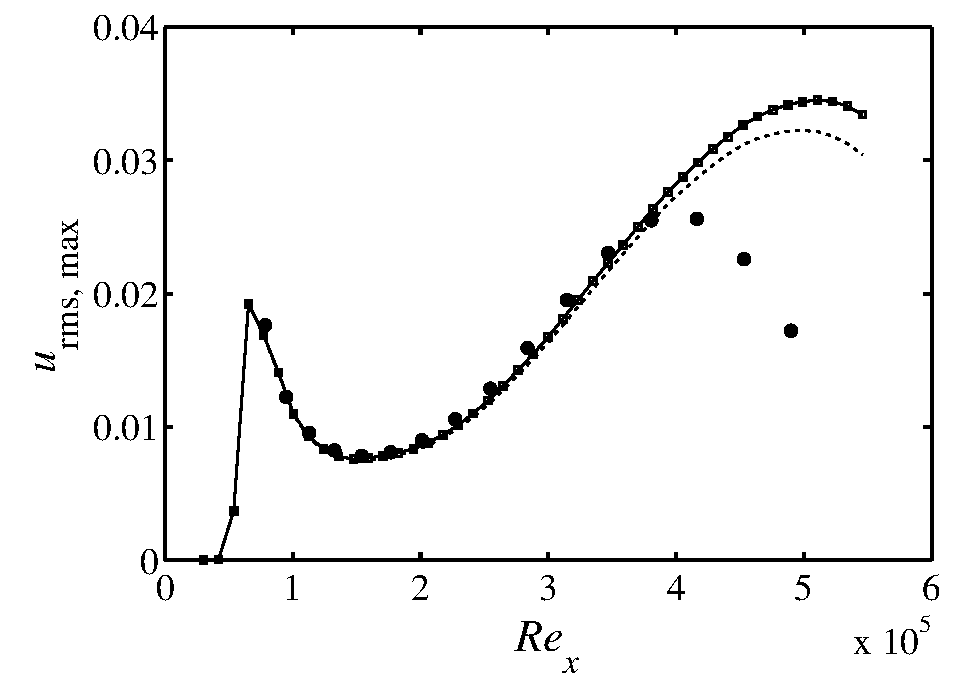
\includegraphics[scale=0.33]{ts_1}
b)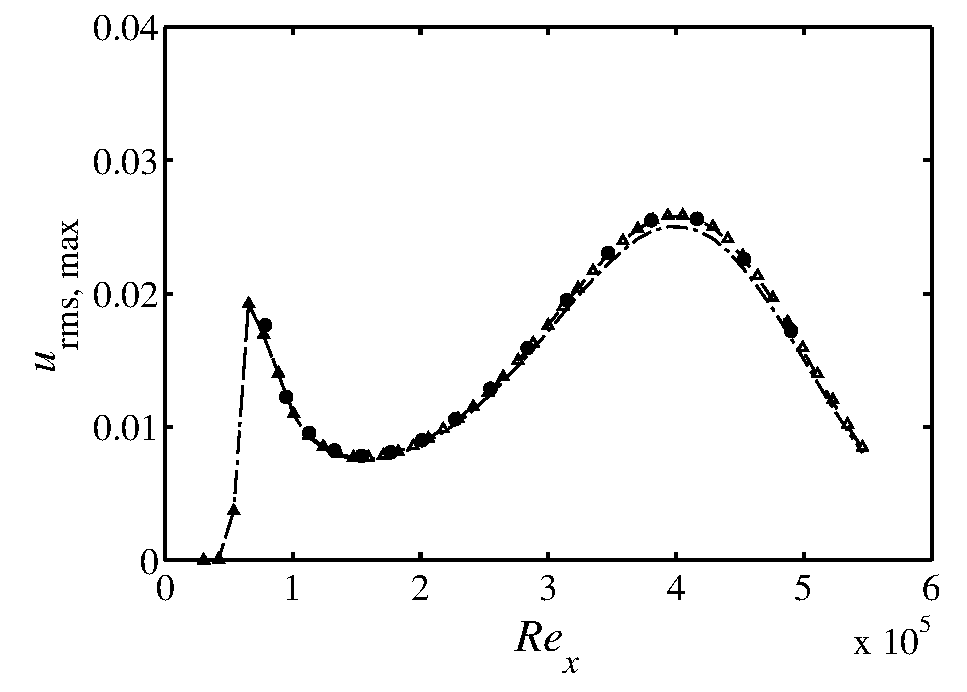
\includegraphics[scale=0.33]{ts_2}
\caption{a) Nonlinear and b) linear development of a two-dimensional
TS-wave in a spatially developing Blasius boundary layer (example
\epath{spatial-blasius-TS}). Wall-normal maximum of the streamwise rms
fluctuation $u_\mathrm{rms,max}$ is shown as a function of the
downstream distance $\mathit{Re}_x$. \solid Direct nonlinear solution;
$\square$ nonlinear solution in disturbance formulation using a
converged baseflow; \dotted nonlinear solution in disturbance
formulation using the Blasius solution as baseflow. \dashed Linearized
disturbance formulation using a converged baseflow; $\Delta$ rescaled
full solution at $10\times$ lower amplitude; \dotdashed linearized
disturbance formulation using the Blasius solution as
baseflow. $\bullet$ Results from linear parabolized stability
equations (PSE).}
\label{fig:example_blasius}
\end{figure}

A sample result displaying the evolution of the streamwise fluctuation
maximum $u_\mathrm{rms,max}$ (option $-71$ in \esoft{pxyst}) is given
in figure \ref{fig:example_blasius}, where the simulation data are
compared to the results obtained from linear PSE (parabolized
stability equations). It can be seen in figure
\ref{fig:example_blasius}a) that the direct nonlinear solution of the
Navier--Stokes equations (\efile{bls.i.full} and \efile{bla.i.full})
gives exactly the same result as the one computed nonlinearly in
disturbance formulation (\efile{bls.i.dist} and \efile{bla.i.pert}),
provided that the corresponding baseflow is a converged solution
(\emph{i.e.}\ obtained using \efile{bls.i.full} and
\efile{bla.i.baseflow}). The growth rate is considerably
underestimated if the Blasius solution (\emph{i.e.}\ a solution to the
boundary layer equations) is used as a baseflow (\efile{bls.i.pert}
and \efile{bla.i.magic-forcing}). On the other hand, due to nonlinear
saturation the nonlinear development is considerably different from
the linear development depicted in figure \ref{fig:example_blasius}b):
The linearized solution around a converged baseflow
(\efile{bla.i.pert-linear}) and the rescaled direct solution coincide
with the linear PSE solution, whereas the linear solution around the
Blasius baseflow is again underestimating the growth of the TS-wave.

An example of a spatially evolving, zero-pressure-gradient turbulent
boundary layer with various passive scalars is provided in
\epath{spatial-blasius-scalars}. The inflow is located at
$\mathit{Re}_{\delta^*_0}=450$. Turbulent statistics, spanwise
two-point correlations and time series at selected coordinates of
various quantities are generated as output. The laminar flow close to
the inlet plane is disturbed via a trip force (see equation
(\ref{eq:trip}) in Section \ref{sec:blafile}) located at $x=10$. The
Prandtl numbers $\mathit{Pr}$ for the scalars are all set to 0.71, and
different boundary conditions have been chosen at the wall and in the
freestream: Dirichlet-Dirichlet, Neumann-Dirichlet, Dirichlet-Neumann
and Neumann-Neumann. Note that the spatial resolution in \efile{par.f}
is not sufficient for a fully-resolved direct numerical simulation.

A similar turbulent boundary layer with large-eddy simulation (LES) is
given as example in \epath{spatial-blasius-les}. In \efile{sgs.i} the
Smagorinsky eddy-viscosity model is turned on together with an
adaptive determination of the model coefficient (dynamic Smagorinsky
model).


% ====================================================================
\section{Spatial Falkner--Skan--Cooke boundary layer flow}
% ====================================================================
In the example \epath{spatial-fsc} the flow from appendix
\ref{sec:temp-fsc-example} is studied in a spatial setting. Traveling
cross-flow vortices are generated, in an upstream location, by
applying a volume force (trip forcing) built as a sum of Stokes modes
with time-varying amplitudes and stochastic coefficients.

The vortices merge and split and form complicated patterns. The time
average of the disturbance energy is plotted in figure
\ref{fig:spatial-fsc} which shows the exponential growth of the
traveling vortices. The fringe forcing starts at $x=350$ and lowers
the perturbation energy and makes the base flow periodic.
\begin{figure}[h]
\setlength{\unitlength}{1mm}
\centering
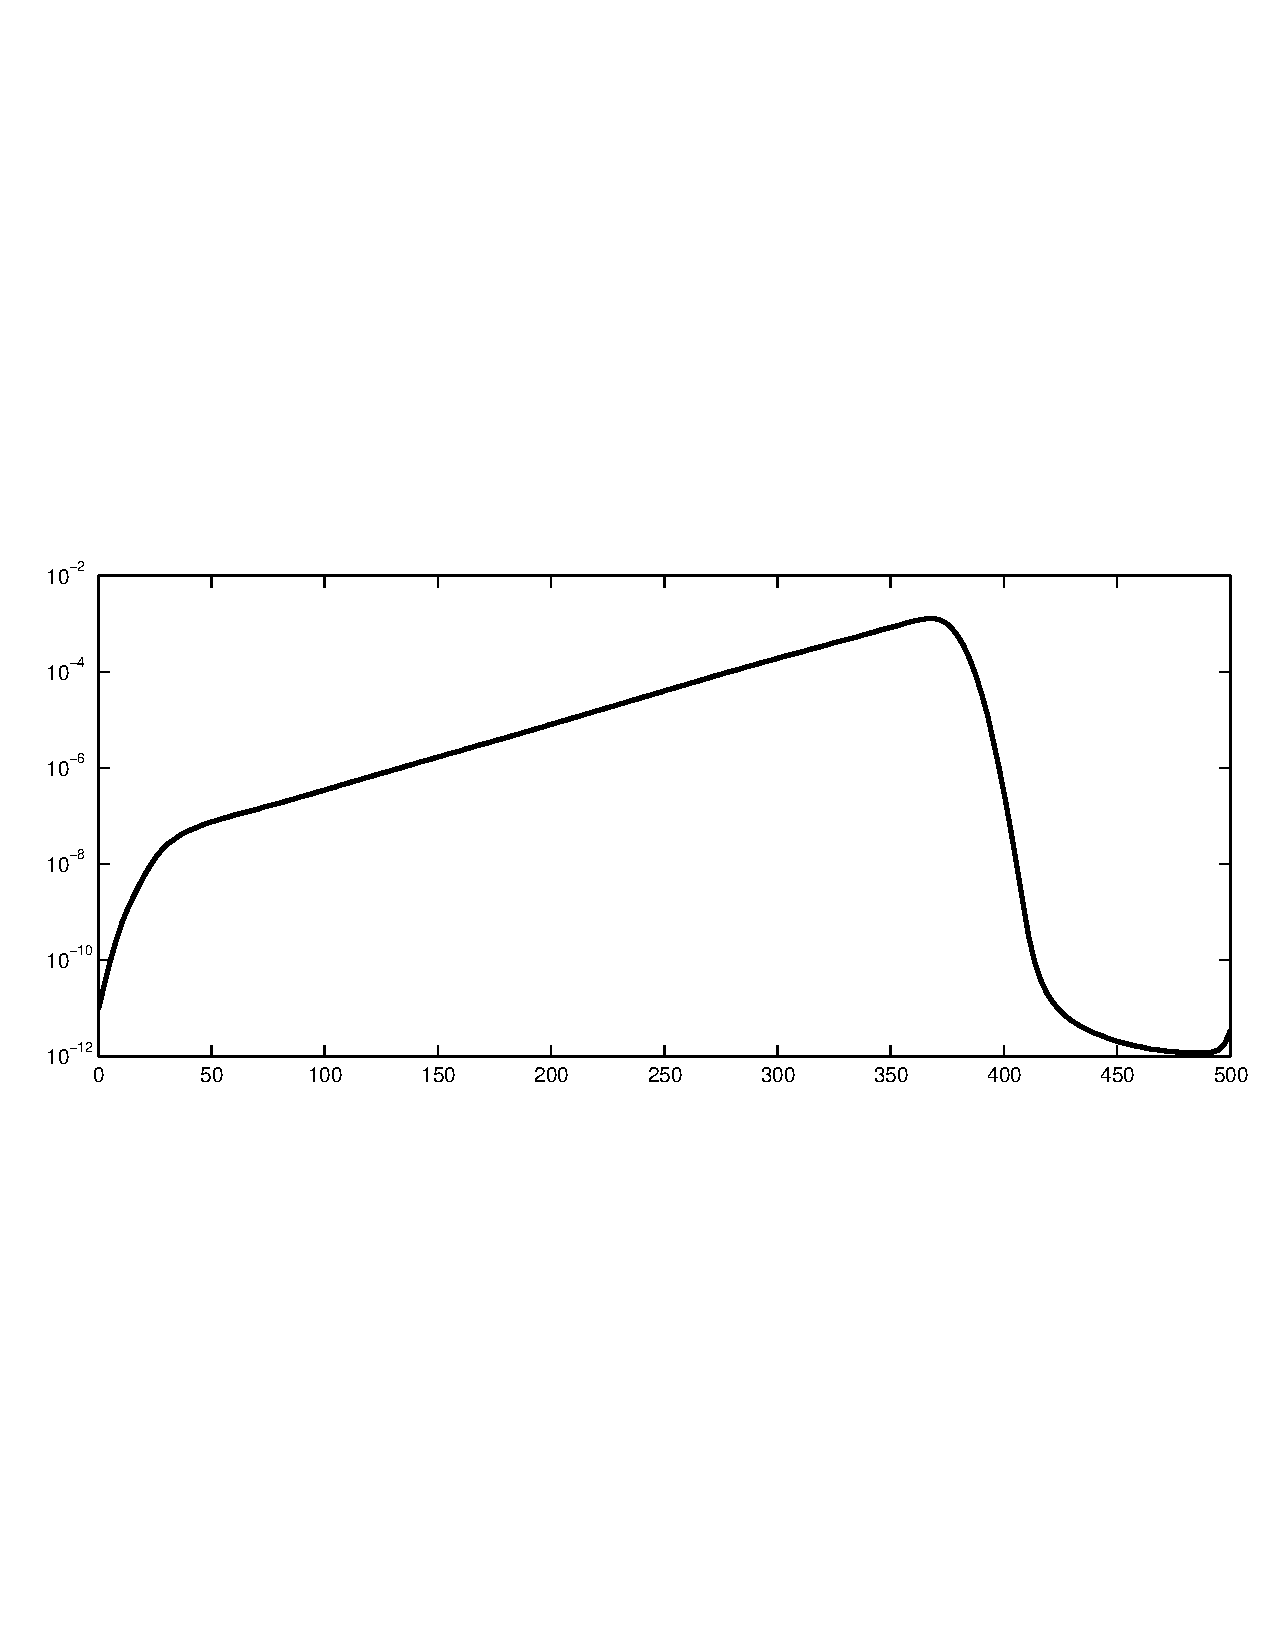
\includegraphics[width=0.85\textwidth]{fsc-spatial-growth}
\put(-107,22){$E$}
\put(-50,-3){$x$}
\caption{Time average of energy integrated in the $z$-direction for
simulation of traveling cross-flow vortices.}
\label{fig:spatial-fsc}
\end{figure} 

The same flow case was studied in \cite{Hogberg-Henningson:98},
\cite{mhogberg:dhenningson} and
\cite{chevalier:hoepffner:akervik:henningson:2007}. In the two latter
studies this flow configuration served as an example to illustrate the
effectiveness of control and compensator algorithms respectively, where
blowing and suction on the lower wall was used to decrease the
disturbance energy growth.


% ####################################################################
\chapter{Scaling of variables}\label{sec:scale}
% ####################################################################
For all the boundary layer flows the scaling, for all parameters, is
based on the displacement boundary layer thickness and free-stream
velocity at $t=0$, $x=0$ for the reference or base flow.  However,
internally in the simulation code \esoft{bla} the implementation uses
a scaling based on the half box height (the external and internal
velocity scale is the same). This means that all external data must be
rescaled when read into the program, and the reverse scaling applied
on output. If we let \epar{dstar} be the displacement thickness
expressed in half box heights, then the following scaling
relationships hold:
\begin{equation}
\begin{aligned}
\text{time}_{\text{int}}      & = \text{time}_{\text{ext}}\times\text{dstar}\,,\\
\text{length}_{\text{int}}    & = \text{length}_{\text{ext}}\times\text{dstar}\,,\\
\text{velocity}_{\text{int}}  & = \text{velocity}_{\text{ext}}\,,\\
\text{vorticity}_{\text{int}} & = \text{vorticity}_{\text{ext}}/\text{dstar}\,,\\
\text{force}_{\text{int}}     & = \text{force}_{\text{ext}}/\text{dstar}\,.
\end{aligned}
\end{equation}
All formatted input and output files except the wave amplitude file
use external scaling, whereas the unformatted files and the wave
amplitude file use internal scaling.

\end{document}
